%% Manuscript for Computers & Security (Elsevier), prepared with the elsarticle class.
%% Journal requirements followed: single-anonymized review (author details on the title page),
%% abstract <= 250 words, <= 12,000 words including abstract, main text, references and
%% appendices (supplementary material is a separate file), highlights as a separate file
%% (highlights.txt), and the declarations required at submission (end of this file).
\documentclass[preprint,12pt,authoryear]{elsarticle}
\usepackage[T1]{fontenc}
\usepackage{lmodern}
\usepackage{microtype}
\usepackage{amsmath,amssymb,amsthm,bm}
\usepackage{graphicx,booktabs,multirow,siunitx,xcolor}
\usepackage{tikz}
\usetikzlibrary{arrows.meta,positioning,fit,backgrounds,calc}
\usepackage[hidelinks]{hyperref}
\usepackage{algorithm,algpseudocode}
\usepackage[capitalise]{cleveref}
\usepackage{lineno}
\linenumbers
\sisetup{detect-all}
\setlength{\emergencystretch}{3em}
\newtheorem{proposition}{Proposition}
\newtheorem{definition}{Definition}
% generated by scripts/make_numbers.py -- do not edit
\newcommand{\CPUmodel}{x86-64 CPU}
\newcommand{\HAIL}{9}
\newcommand{\HAId}{57}
\newcommand{\SimHazMax}{1039}
\newcommand{\SimHazMedian}{301}
\newcommand{\SimHazMin}{6}
\newcommand{\SimNattacks}{280}
\newcommand{\SimNhaz}{113}
\newcommand{\dclhaiCLXdclfixedOneTwoZerotea}{0.34}
\newcommand{\dclhaiCLXdclfixedSixZerosingle}{0.34}
\newcommand{\dclhaiCLXdclfixedSixZerotea}{0.32}
\newcommand{\dclhaiCLXdclfixedSixZeroteahrthree}{0.61}
\newcommand{\dclhaiCLXdclfixedThreeZerotea}{0.30}
\newcommand{\dclhaiFungensdclfixedOneTwoZerotea}{0.62}
\newcommand{\dclhaiFungensdclfixedSixZerosingle}{0.51}
\newcommand{\dclhaiFungensdclfixedSixZerotea}{0.54}
\newcommand{\dclhaiFungensdclfixedSixZeroteahrthree}{0.72}
\newcommand{\dclhaiFungensdclfixedThreeZerotea}{0.54}
\newcommand{\dclhaiIGdclfixedOneTwoZerotea}{0.63}
\newcommand{\dclhaiIGdclfixedSixZerosingle}{0.49}
\newcommand{\dclhaiIGdclfixedSixZerotea}{0.54}
\newcommand{\dclhaiIGdclfixedSixZeroteahrthree}{0.68}
\newcommand{\dclhaiIGdclfixedThreeZerotea}{0.51}
\newcommand{\dclhaiKSOneZeroTwoFourdclfixedOneTwoZerotea}{0.59}
\newcommand{\dclhaiKSOneZeroTwoFourdclfixedSixZerosingle}{0.46}
\newcommand{\dclhaiKSOneZeroTwoFourdclfixedSixZerotea}{0.51}
\newcommand{\dclhaiKSOneZeroTwoFourdclfixedSixZeroteahrthree}{0.68}
\newcommand{\dclhaiKSOneZeroTwoFourdclfixedThreeZerotea}{0.49}
\newcommand{\dclhaiKSeqdclfixedOneTwoZerotea}{0.55}
\newcommand{\dclhaiKSeqdclfixedSixZerosingle}{0.41}
\newcommand{\dclhaiKSeqdclfixedSixZerotea}{0.48}
\newcommand{\dclhaiKSeqdclfixedSixZeroteahrthree}{0.67}
\newcommand{\dclhaiKSeqdclfixedThreeZerotea}{0.47}
\newcommand{\dclhaiLIMEOneZeroTwoFourdclfixedOneTwoZerotea}{0.60}
\newcommand{\dclhaiLIMEOneZeroTwoFourdclfixedSixZerosingle}{0.50}
\newcommand{\dclhaiLIMEOneZeroTwoFourdclfixedSixZerotea}{0.52}
\newcommand{\dclhaiLIMEOneZeroTwoFourdclfixedSixZeroteahrthree}{0.69}
\newcommand{\dclhaiLIMEOneZeroTwoFourdclfixedThreeZerotea}{0.51}
\newcommand{\dclhaiLIMEeqdclfixedOneTwoZerotea}{0.60}
\newcommand{\dclhaiLIMEeqdclfixedSixZerosingle}{0.48}
\newcommand{\dclhaiLIMEeqdclfixedSixZerotea}{0.52}
\newcommand{\dclhaiLIMEeqdclfixedSixZeroteahrthree}{0.68}
\newcommand{\dclhaiLIMEeqdclfixedThreeZerotea}{0.50}
\newcommand{\dclhaiLXbgdclfixedOneTwoZerotea}{0.60}
\newcommand{\dclhaiLXbgdclfixedSixZerosingle}{0.51}
\newcommand{\dclhaiLXbgdclfixedSixZerotea}{0.53}
\newcommand{\dclhaiLXbgdclfixedSixZeroteahrthree}{0.70}
\newcommand{\dclhaiLXbgdclfixedThreeZerotea}{0.51}
\newcommand{\dclhaiLXdclfixedOneTwoZerotea}{0.60}
\newcommand{\dclhaiLXdclfixedSixZerosingle}{0.51}
\newcommand{\dclhaiLXdclfixedSixZerotea}{0.53}
\newcommand{\dclhaiLXdclfixedSixZeroteahrthree}{0.70}
\newcommand{\dclhaiLXdclfixedThreeZerotea}{0.51}
\newcommand{\dclhaiREdclfixedOneTwoZerotea}{0.51}
\newcommand{\dclhaiREdclfixedSixZerosingle}{0.46}
\newcommand{\dclhaiREdclfixedSixZerotea}{0.50}
\newcommand{\dclhaiREdclfixedSixZeroteahrthree}{0.68}
\newcommand{\dclhaiREdclfixedThreeZerotea}{0.46}
\newcommand{\dclhaiRPXdclfixedOneTwoZerotea}{0.17}
\newcommand{\dclhaiRPXdclfixedSixZerosingle}{0.17}
\newcommand{\dclhaiRPXdclfixedSixZerotea}{0.19}
\newcommand{\dclhaiRPXdclfixedSixZeroteahrthree}{0.52}
\newcommand{\dclhaiRPXdclfixedThreeZerotea}{0.16}
\newcommand{\dclhaiSMdclfixedOneTwoZerotea}{0.39}
\newcommand{\dclhaiSMdclfixedSixZerosingle}{0.31}
\newcommand{\dclhaiSMdclfixedSixZerotea}{0.32}
\newcommand{\dclhaiSMdclfixedSixZeroteahrthree}{0.49}
\newcommand{\dclhaiSMdclfixedThreeZerotea}{0.32}
\newcommand{\dclsimCLXdclfixedOneTwoZerotea}{0.10}
\newcommand{\dclsimCLXdclfixedSixZerosingle}{0.09}
\newcommand{\dclsimCLXdclfixedSixZerotea}{0.10}
\newcommand{\dclsimCLXdclfixedSixZeroteahrthree}{0.41}
\newcommand{\dclsimCLXdclfixedThreeZerotea}{0.10}
\newcommand{\dclsimCLXdclhazhzsingle}{0.10}
\newcommand{\dclsimCLXdclhazhztea}{0.14}
\newcommand{\dclsimCLXdclhazhzteahrthree}{0.38}
\newcommand{\dclsimFungensdclfixedOneTwoZerotea}{0.50}
\newcommand{\dclsimFungensdclfixedSixZerosingle}{0.23}
\newcommand{\dclsimFungensdclfixedSixZerotea}{0.50}
\newcommand{\dclsimFungensdclfixedSixZeroteahrthree}{0.53}
\newcommand{\dclsimFungensdclfixedThreeZerotea}{0.50}
\newcommand{\dclsimFungensdclhazhzsingle}{0.21}
\newcommand{\dclsimFungensdclhazhztea}{0.44}
\newcommand{\dclsimFungensdclhazhzteahrthree}{0.54}
\newcommand{\dclsimIGdclfixedOneTwoZerotea}{0.52}
\newcommand{\dclsimIGdclfixedSixZerosingle}{0.34}
\newcommand{\dclsimIGdclfixedSixZerotea}{0.52}
\newcommand{\dclsimIGdclfixedSixZeroteahrthree}{0.53}
\newcommand{\dclsimIGdclfixedThreeZerotea}{0.51}
\newcommand{\dclsimIGdclhazhzsingle}{0.33}
\newcommand{\dclsimIGdclhazhztea}{0.50}
\newcommand{\dclsimIGdclhazhzteahrthree}{0.54}
\newcommand{\dclsimKSOneZeroTwoFourdclfixedOneTwoZerotea}{0.48}
\newcommand{\dclsimKSOneZeroTwoFourdclfixedSixZerosingle}{0.24}
\newcommand{\dclsimKSOneZeroTwoFourdclfixedSixZerotea}{0.48}
\newcommand{\dclsimKSOneZeroTwoFourdclfixedSixZeroteahrthree}{0.52}
\newcommand{\dclsimKSOneZeroTwoFourdclfixedThreeZerotea}{0.48}
\newcommand{\dclsimKSOneZeroTwoFourdclhazhzsingle}{0.22}
\newcommand{\dclsimKSOneZeroTwoFourdclhazhztea}{0.43}
\newcommand{\dclsimKSOneZeroTwoFourdclhazhzteahrthree}{0.51}
\newcommand{\dclsimKSeqdclfixedOneTwoZerotea}{0.40}
\newcommand{\dclsimKSeqdclfixedSixZerosingle}{0.23}
\newcommand{\dclsimKSeqdclfixedSixZerotea}{0.40}
\newcommand{\dclsimKSeqdclfixedSixZeroteahrthree}{0.48}
\newcommand{\dclsimKSeqdclfixedThreeZerotea}{0.40}
\newcommand{\dclsimKSeqdclhazhzsingle}{0.25}
\newcommand{\dclsimKSeqdclhazhztea}{0.40}
\newcommand{\dclsimKSeqdclhazhzteahrthree}{0.51}
\newcommand{\dclsimLIMEOneZeroTwoFourdclfixedOneTwoZerotea}{0.50}
\newcommand{\dclsimLIMEOneZeroTwoFourdclfixedSixZerosingle}{0.24}
\newcommand{\dclsimLIMEOneZeroTwoFourdclfixedSixZerotea}{0.50}
\newcommand{\dclsimLIMEOneZeroTwoFourdclfixedSixZeroteahrthree}{0.53}
\newcommand{\dclsimLIMEOneZeroTwoFourdclfixedThreeZerotea}{0.50}
\newcommand{\dclsimLIMEOneZeroTwoFourdclhazhzsingle}{0.22}
\newcommand{\dclsimLIMEOneZeroTwoFourdclhazhztea}{0.46}
\newcommand{\dclsimLIMEOneZeroTwoFourdclhazhzteahrthree}{0.52}
\newcommand{\dclsimLIMEeqdclfixedOneTwoZerotea}{0.42}
\newcommand{\dclsimLIMEeqdclfixedSixZerosingle}{0.21}
\newcommand{\dclsimLIMEeqdclfixedSixZerotea}{0.42}
\newcommand{\dclsimLIMEeqdclfixedSixZeroteahrthree}{0.50}
\newcommand{\dclsimLIMEeqdclfixedThreeZerotea}{0.42}
\newcommand{\dclsimLIMEeqdclhazhzsingle}{0.20}
\newcommand{\dclsimLIMEeqdclhazhztea}{0.38}
\newcommand{\dclsimLIMEeqdclhazhzteahrthree}{0.48}
\newcommand{\dclsimLXbgdclfixedOneTwoZerotea}{0.52}
\newcommand{\dclsimLXbgdclfixedSixZerosingle}{0.28}
\newcommand{\dclsimLXbgdclfixedSixZerotea}{0.52}
\newcommand{\dclsimLXbgdclfixedSixZeroteahrthree}{0.53}
\newcommand{\dclsimLXbgdclfixedThreeZerotea}{0.51}
\newcommand{\dclsimLXbgdclhazhzsingle}{0.29}
\newcommand{\dclsimLXbgdclhazhztea}{0.49}
\newcommand{\dclsimLXbgdclhazhzteahrthree}{0.54}
\newcommand{\dclsimLXdclfixedOneTwoZerotea}{0.51}
\newcommand{\dclsimLXdclfixedSixZerosingle}{0.27}
\newcommand{\dclsimLXdclfixedSixZerotea}{0.52}
\newcommand{\dclsimLXdclfixedSixZeroteahrthree}{0.53}
\newcommand{\dclsimLXdclfixedThreeZerotea}{0.51}
\newcommand{\dclsimLXdclhazhzsingle}{0.28}
\newcommand{\dclsimLXdclhazhztea}{0.48}
\newcommand{\dclsimLXdclhazhzteahrthree}{0.53}
\newcommand{\dclsimREdclfixedOneTwoZerotea}{0.50}
\newcommand{\dclsimREdclfixedSixZerosingle}{0.21}
\newcommand{\dclsimREdclfixedSixZerotea}{0.49}
\newcommand{\dclsimREdclfixedSixZeroteahrthree}{0.53}
\newcommand{\dclsimREdclfixedThreeZerotea}{0.49}
\newcommand{\dclsimREdclhazhzsingle}{0.17}
\newcommand{\dclsimREdclhazhztea}{0.41}
\newcommand{\dclsimREdclhazhzteahrthree}{0.54}
\newcommand{\dclsimRPXdclfixedOneTwoZerotea}{0.35}
\newcommand{\dclsimRPXdclfixedSixZerosingle}{0.17}
\newcommand{\dclsimRPXdclfixedSixZerotea}{0.33}
\newcommand{\dclsimRPXdclfixedSixZeroteahrthree}{0.51}
\newcommand{\dclsimRPXdclfixedThreeZerotea}{0.32}
\newcommand{\dclsimRPXdclhazhzsingle}{0.17}
\newcommand{\dclsimRPXdclhazhztea}{0.29}
\newcommand{\dclsimRPXdclhazhzteahrthree}{0.50}
\newcommand{\dclsimSMdclfixedOneTwoZerotea}{0.47}
\newcommand{\dclsimSMdclfixedSixZerosingle}{0.21}
\newcommand{\dclsimSMdclfixedSixZerotea}{0.46}
\newcommand{\dclsimSMdclfixedSixZeroteahrthree}{0.53}
\newcommand{\dclsimSMdclfixedThreeZerotea}{0.47}
\newcommand{\dclsimSMdclhazhzsingle}{0.19}
\newcommand{\dclsimSMdclhazhztea}{0.40}
\newcommand{\dclsimSMdclhazhzteahrthree}{0.54}
\newcommand{\detHaiCnnER}{0.89}
\newcommand{\detHaiCnnFA}{0.34}
\newcommand{\detHaiGruER}{0.90}
\newcommand{\detHaiGruFA}{0.36}
\newcommand{\detHaiLinearER}{0.92}
\newcommand{\detHaiLinearFA}{0.42}
\newcommand{\detHaiMlpER}{0.90}
\newcommand{\detHaiMlpFA}{0.36}
\newcommand{\detSimCnnER}{0.89}
\newcommand{\detSimCnnFA}{0.96}
\newcommand{\detSimGruER}{0.93}
\newcommand{\detSimGruFA}{0.89}
\newcommand{\detSimLinearER}{0.96}
\newcommand{\detSimLinearFA}{1.38}
\newcommand{\detSimMlpER}{0.76}
\newcommand{\detSimMlpFA}{0.31}
\newcommand{\evalshaiShaTS}{\textbf{??}}
\newcommand{\intimeDeliveredFungens}{0.80}
\newcommand{\intimeDeliveredIG}{0.90}
\newcommand{\intimeDeliveredKSOneZeroTwoFour}{0.78}
\newcommand{\intimeDeliveredLX}{0.87}
\newcommand{\intimeDeliveredLXbg}{0.89}
\newcommand{\intimeDeliveredRE}{0.74}
\newcommand{\intimeFail}{704}
\newcommand{\intimeFailUndelivered}{603}
\newcommand{\intimeFailUndeliveredPct}{86}
\newcommand{\latshaiShaTScnn}{\textbf{??}}
\newcommand{\leakBlockedAP}{0.624}
\newcommand{\leakBlockedAPsd}{0.026}
\newcommand{\leakBlockedAUC}{0.946}
\newcommand{\leakBlockedAUCsd}{0.003}
\newcommand{\leakBlockedFOne}{0.575}
\newcommand{\leakBlockedFOnesd}{0.029}
\newcommand{\leakRandomAP}{0.983}
\newcommand{\leakRandomAPsd}{0.006}
\newcommand{\leakRandomAUC}{0.998}
\newcommand{\leakRandomAUCsd}{0.001}
\newcommand{\leakRandomFOne}{0.940}
\newcommand{\leakRandomFOnesd}{0.008}
\newcommand{\lochaiCLXalarmOneEightZerosinglehrOne}{0.20}
\newcommand{\lochaiCLXalarmOneEightZeroteahrOne}{0.38}
\newcommand{\lochaiCLXalarmSixZerosinglehrOne}{0.39}
\newcommand{\lochaiCLXalarmSixZeroteahrOne}{0.38}
\newcommand{\lochaiCLXalarmSixZeroteahrThree}{0.79}
\newcommand{\lochaiCLXalarmSixZeroteanr}{0.18}
\newcommand{\lochaiCLXalarmZerosinglehrOne}{0.45}
\newcommand{\lochaiCLXbestguesssinglehrOne}{0.31}
\newcommand{\lochaiFungensalarmOneEightZerosinglehrOne}{0.34}
\newcommand{\lochaiFungensalarmOneEightZeroteahrOne}{0.71}
\newcommand{\lochaiFungensalarmSixZerosinglehrOne}{0.56}
\newcommand{\lochaiFungensalarmSixZeroteahrOne}{0.72}
\newcommand{\lochaiFungensalarmSixZeroteahrThree}{0.92}
\newcommand{\lochaiFungensalarmSixZeroteanr}{0.07}
\newcommand{\lochaiFungensalarmZerosinglehrOne}{0.76}
\newcommand{\lochaiFungensbestguesssinglehrOne}{0.60}
\newcommand{\lochaiIGalarmOneEightZerosinglehrOne}{0.33}
\newcommand{\lochaiIGalarmOneEightZeroteahrOne}{0.70}
\newcommand{\lochaiIGalarmSixZerosinglehrOne}{0.56}
\newcommand{\lochaiIGalarmSixZeroteahrOne}{0.72}
\newcommand{\lochaiIGalarmSixZeroteahrThree}{0.93}
\newcommand{\lochaiIGalarmSixZeroteanr}{0.06}
\newcommand{\lochaiIGalarmZerosinglehrOne}{0.75}
\newcommand{\lochaiIGbestguesssinglehrOne}{0.50}
\newcommand{\lochaiKSOneZeroTwoFouralarmOneEightZerosinglehrOne}{0.28}
\newcommand{\lochaiKSOneZeroTwoFouralarmOneEightZeroteahrOne}{0.65}
\newcommand{\lochaiKSOneZeroTwoFouralarmSixZerosinglehrOne}{0.51}
\newcommand{\lochaiKSOneZeroTwoFouralarmSixZeroteahrOne}{0.69}
\newcommand{\lochaiKSOneZeroTwoFouralarmSixZeroteahrThree}{0.92}
\newcommand{\lochaiKSOneZeroTwoFouralarmSixZeroteanr}{0.07}
\newcommand{\lochaiKSOneZeroTwoFouralarmZerosinglehrOne}{0.74}
\newcommand{\lochaiKSOneZeroTwoFourbestguesssinglehrOne}{0.48}
\newcommand{\lochaiKSeqalarmOneEightZerosinglehrOne}{0.22}
\newcommand{\lochaiKSeqalarmOneEightZeroteahrOne}{0.60}
\newcommand{\lochaiKSeqalarmSixZerosinglehrOne}{0.50}
\newcommand{\lochaiKSeqalarmSixZeroteahrOne}{0.64}
\newcommand{\lochaiKSeqalarmSixZeroteahrThree}{0.90}
\newcommand{\lochaiKSeqalarmSixZeroteanr}{0.09}
\newcommand{\lochaiKSeqalarmZerosinglehrOne}{0.70}
\newcommand{\lochaiKSeqbestguesssinglehrOne}{0.47}
\newcommand{\lochaiLIMEOneZeroTwoFouralarmOneEightZerosinglehrOne}{0.31}
\newcommand{\lochaiLIMEOneZeroTwoFouralarmOneEightZeroteahrOne}{0.66}
\newcommand{\lochaiLIMEOneZeroTwoFouralarmSixZerosinglehrOne}{0.56}
\newcommand{\lochaiLIMEOneZeroTwoFouralarmSixZeroteahrOne}{0.69}
\newcommand{\lochaiLIMEOneZeroTwoFouralarmSixZeroteahrThree}{0.93}
\newcommand{\lochaiLIMEOneZeroTwoFouralarmSixZeroteanr}{0.07}
\newcommand{\lochaiLIMEOneZeroTwoFouralarmZerosinglehrOne}{0.76}
\newcommand{\lochaiLIMEOneZeroTwoFourbestguesssinglehrOne}{0.49}
\newcommand{\lochaiLIMEeqalarmOneEightZerosinglehrOne}{0.26}
\newcommand{\lochaiLIMEeqalarmOneEightZeroteahrOne}{0.66}
\newcommand{\lochaiLIMEeqalarmSixZerosinglehrOne}{0.55}
\newcommand{\lochaiLIMEeqalarmSixZeroteahrOne}{0.70}
\newcommand{\lochaiLIMEeqalarmSixZeroteahrThree}{0.93}
\newcommand{\lochaiLIMEeqalarmSixZeroteanr}{0.07}
\newcommand{\lochaiLIMEeqalarmZerosinglehrOne}{0.75}
\newcommand{\lochaiLIMEeqbestguesssinglehrOne}{0.49}
\newcommand{\lochaiLXalarmOneEightZerosinglehrOne}{0.30}
\newcommand{\lochaiLXalarmOneEightZeroteahrOne}{0.64}
\newcommand{\lochaiLXalarmSixZerosinglehrOne}{0.60}
\newcommand{\lochaiLXalarmSixZeroteahrOne}{0.70}
\newcommand{\lochaiLXalarmSixZeroteahrThree}{0.94}
\newcommand{\lochaiLXalarmSixZeroteanr}{0.06}
\newcommand{\lochaiLXalarmZerosinglehrOne}{0.79}
\newcommand{\lochaiLXbestguesssinglehrOne}{0.47}
\newcommand{\lochaiLXbgalarmOneEightZerosinglehrOne}{0.31}
\newcommand{\lochaiLXbgalarmOneEightZeroteahrOne}{0.65}
\newcommand{\lochaiLXbgalarmSixZerosinglehrOne}{0.58}
\newcommand{\lochaiLXbgalarmSixZeroteahrOne}{0.71}
\newcommand{\lochaiLXbgalarmSixZeroteahrThree}{0.94}
\newcommand{\lochaiLXbgalarmSixZeroteanr}{0.06}
\newcommand{\lochaiLXbgalarmZerosinglehrOne}{0.74}
\newcommand{\lochaiLXbgbestguesssinglehrOne}{0.55}
\newcommand{\lochaiREalarmOneEightZerosinglehrOne}{0.35}
\newcommand{\lochaiREalarmOneEightZeroteahrOne}{0.57}
\newcommand{\lochaiREalarmSixZerosinglehrOne}{0.48}
\newcommand{\lochaiREalarmSixZeroteahrOne}{0.61}
\newcommand{\lochaiREalarmSixZeroteahrThree}{0.89}
\newcommand{\lochaiREalarmSixZeroteanr}{0.09}
\newcommand{\lochaiREalarmZerosinglehrOne}{0.71}
\newcommand{\lochaiREbestguesssinglehrOne}{0.49}
\newcommand{\lochaiRPXalarmOneEightZerosinglehrOne}{0.16}
\newcommand{\lochaiRPXalarmOneEightZeroteahrOne}{0.17}
\newcommand{\lochaiRPXalarmSixZerosinglehrOne}{0.19}
\newcommand{\lochaiRPXalarmSixZeroteahrOne}{0.21}
\newcommand{\lochaiRPXalarmSixZeroteahrThree}{0.68}
\newcommand{\lochaiRPXalarmSixZeroteanr}{0.26}
\newcommand{\lochaiRPXalarmZerosinglehrOne}{0.25}
\newcommand{\lochaiRPXbestguesssinglehrOne}{0.17}
\newcommand{\lochaiSMalarmOneEightZerosinglehrOne}{0.22}
\newcommand{\lochaiSMalarmOneEightZeroteahrOne}{0.44}
\newcommand{\lochaiSMalarmSixZerosinglehrOne}{0.32}
\newcommand{\lochaiSMalarmSixZeroteahrOne}{0.44}
\newcommand{\lochaiSMalarmSixZeroteahrThree}{0.67}
\newcommand{\lochaiSMalarmSixZeroteanr}{0.27}
\newcommand{\lochaiSMalarmZerosinglehrOne}{0.43}
\newcommand{\lochaiSMbestguesssinglehrOne}{0.43}
\newcommand{\locsimCLXalarmOneEightZerosinglehrOne}{0.14}
\newcommand{\locsimCLXalarmOneEightZeroteahrOne}{0.23}
\newcommand{\locsimCLXalarmSixZerosinglehrOne}{0.16}
\newcommand{\locsimCLXalarmSixZeroteahrOne}{0.23}
\newcommand{\locsimCLXalarmSixZeroteahrThree}{0.78}
\newcommand{\locsimCLXalarmSixZeroteanr}{0.31}
\newcommand{\locsimCLXalarmZerosinglehrOne}{0.27}
\newcommand{\locsimCLXbestguesssinglehrOne}{0.12}
\newcommand{\locsimFungensalarmOneEightZerosinglehrOne}{0.45}
\newcommand{\locsimFungensalarmOneEightZeroteahrOne}{0.82}
\newcommand{\locsimFungensalarmSixZerosinglehrOne}{0.49}
\newcommand{\locsimFungensalarmSixZeroteahrOne}{0.82}
\newcommand{\locsimFungensalarmSixZeroteahrThree}{0.97}
\newcommand{\locsimFungensalarmSixZeroteanr}{0.06}
\newcommand{\locsimFungensalarmZerosinglehrOne}{0.87}
\newcommand{\locsimFungensbestguesssinglehrOne}{0.48}
\newcommand{\locsimIGalarmOneEightZerosinglehrOne}{0.55}
\newcommand{\locsimIGalarmOneEightZeroteahrOne}{0.83}
\newcommand{\locsimIGalarmSixZerosinglehrOne}{0.66}
\newcommand{\locsimIGalarmSixZeroteahrOne}{0.84}
\newcommand{\locsimIGalarmSixZeroteahrThree}{0.96}
\newcommand{\locsimIGalarmSixZeroteanr}{0.06}
\newcommand{\locsimIGalarmZerosinglehrOne}{0.86}
\newcommand{\locsimIGbestguesssinglehrOne}{0.68}
\newcommand{\locsimKSOneZeroTwoFouralarmOneEightZerosinglehrOne}{0.43}
\newcommand{\locsimKSOneZeroTwoFouralarmOneEightZeroteahrOne}{0.77}
\newcommand{\locsimKSOneZeroTwoFouralarmSixZerosinglehrOne}{0.50}
\newcommand{\locsimKSOneZeroTwoFouralarmSixZeroteahrOne}{0.80}
\newcommand{\locsimKSOneZeroTwoFouralarmSixZeroteahrThree}{0.93}
\newcommand{\locsimKSOneZeroTwoFouralarmSixZeroteanr}{0.09}
\newcommand{\locsimKSOneZeroTwoFouralarmZerosinglehrOne}{0.84}
\newcommand{\locsimKSOneZeroTwoFourbestguesssinglehrOne}{0.50}
\newcommand{\locsimKSeqalarmOneEightZerosinglehrOne}{0.40}
\newcommand{\locsimKSeqalarmOneEightZeroteahrOne}{0.69}
\newcommand{\locsimKSeqalarmSixZerosinglehrOne}{0.47}
\newcommand{\locsimKSeqalarmSixZeroteahrOne}{0.71}
\newcommand{\locsimKSeqalarmSixZeroteahrThree}{0.90}
\newcommand{\locsimKSeqalarmSixZeroteanr}{0.13}
\newcommand{\locsimKSeqalarmZerosinglehrOne}{0.80}
\newcommand{\locsimKSeqbestguesssinglehrOne}{0.46}
\newcommand{\locsimLIMEOneZeroTwoFouralarmOneEightZerosinglehrOne}{0.45}
\newcommand{\locsimLIMEOneZeroTwoFouralarmOneEightZeroteahrOne}{0.81}
\newcommand{\locsimLIMEOneZeroTwoFouralarmSixZerosinglehrOne}{0.52}
\newcommand{\locsimLIMEOneZeroTwoFouralarmSixZeroteahrOne}{0.82}
\newcommand{\locsimLIMEOneZeroTwoFouralarmSixZeroteahrThree}{0.95}
\newcommand{\locsimLIMEOneZeroTwoFouralarmSixZeroteanr}{0.07}
\newcommand{\locsimLIMEOneZeroTwoFouralarmZerosinglehrOne}{0.85}
\newcommand{\locsimLIMEOneZeroTwoFourbestguesssinglehrOne}{0.50}
\newcommand{\locsimLIMEeqalarmOneEightZerosinglehrOne}{0.40}
\newcommand{\locsimLIMEeqalarmOneEightZeroteahrOne}{0.70}
\newcommand{\locsimLIMEeqalarmSixZerosinglehrOne}{0.46}
\newcommand{\locsimLIMEeqalarmSixZeroteahrOne}{0.72}
\newcommand{\locsimLIMEeqalarmSixZeroteahrThree}{0.91}
\newcommand{\locsimLIMEeqalarmSixZeroteanr}{0.12}
\newcommand{\locsimLIMEeqalarmZerosinglehrOne}{0.82}
\newcommand{\locsimLIMEeqbestguesssinglehrOne}{0.42}
\newcommand{\locsimLXalarmOneEightZerosinglehrOne}{0.46}
\newcommand{\locsimLXalarmOneEightZeroteahrOne}{0.80}
\newcommand{\locsimLXalarmSixZerosinglehrOne}{0.53}
\newcommand{\locsimLXalarmSixZeroteahrOne}{0.82}
\newcommand{\locsimLXalarmSixZeroteahrThree}{0.95}
\newcommand{\locsimLXalarmSixZeroteanr}{0.07}
\newcommand{\locsimLXalarmZerosinglehrOne}{0.85}
\newcommand{\locsimLXbestguesssinglehrOne}{0.57}
\newcommand{\locsimLXbgalarmOneEightZerosinglehrOne}{0.50}
\newcommand{\locsimLXbgalarmOneEightZeroteahrOne}{0.83}
\newcommand{\locsimLXbgalarmSixZerosinglehrOne}{0.60}
\newcommand{\locsimLXbgalarmSixZeroteahrOne}{0.85}
\newcommand{\locsimLXbgalarmSixZeroteahrThree}{0.96}
\newcommand{\locsimLXbgalarmSixZeroteanr}{0.06}
\newcommand{\locsimLXbgalarmZerosinglehrOne}{0.87}
\newcommand{\locsimLXbgbestguesssinglehrOne}{0.54}
\newcommand{\locsimREalarmOneEightZerosinglehrOne}{0.41}
\newcommand{\locsimREalarmOneEightZeroteahrOne}{0.80}
\newcommand{\locsimREalarmSixZerosinglehrOne}{0.44}
\newcommand{\locsimREalarmSixZeroteahrOne}{0.80}
\newcommand{\locsimREalarmSixZeroteahrThree}{0.96}
\newcommand{\locsimREalarmSixZeroteanr}{0.07}
\newcommand{\locsimREalarmZerosinglehrOne}{0.86}
\newcommand{\locsimREbestguesssinglehrOne}{0.43}
\newcommand{\locsimRPXalarmOneEightZerosinglehrOne}{0.32}
\newcommand{\locsimRPXalarmOneEightZeroteahrOne}{0.58}
\newcommand{\locsimRPXalarmSixZerosinglehrOne}{0.35}
\newcommand{\locsimRPXalarmSixZeroteahrOne}{0.58}
\newcommand{\locsimRPXalarmSixZeroteahrThree}{0.90}
\newcommand{\locsimRPXalarmSixZeroteanr}{0.16}
\newcommand{\locsimRPXalarmZerosinglehrOne}{0.54}
\newcommand{\locsimRPXbestguesssinglehrOne}{0.35}
\newcommand{\locsimSMalarmOneEightZerosinglehrOne}{0.40}
\newcommand{\locsimSMalarmOneEightZeroteahrOne}{0.69}
\newcommand{\locsimSMalarmSixZerosinglehrOne}{0.43}
\newcommand{\locsimSMalarmSixZeroteahrOne}{0.70}
\newcommand{\locsimSMalarmSixZeroteahrThree}{0.95}
\newcommand{\locsimSMalarmSixZeroteanr}{0.10}
\newcommand{\locsimSMalarmZerosinglehrOne}{0.65}
\newcommand{\locsimSMbestguesssinglehrOne}{0.44}
\newcommand{\nhaitestdclSixZerohrOne}{200}
\newcommand{\nhaitesthrOnealarmSixZero}{181}
\newcommand{\nhaitesthrOnealarmZero}{181}
\newcommand{\nhaitesthrOnebestguess}{200}
\newcommand{\nsimtestdclSixZerohrOne}{1120}
\newcommand{\nsimtestdclhazhrOne}{452}
\newcommand{\nsimtesthrOnealarmSixZero}{1014}
\newcommand{\nsimtesthrOnealarmZero}{1014}
\newcommand{\nsimtesthrOnebestguess}{1120}
\newcommand{\phaitestdclSixZerohrOneCLXsingle}{4.3e-07}
\newcommand{\phaitestdclSixZerohrOneCLXtea}{2.0e-07}
\newcommand{\phaitestdclSixZerohrOneFungenssingle}{1.000}
\newcommand{\phaitestdclSixZerohrOneFungenstea}{1.000}
\newcommand{\phaitestdclSixZerohrOneIGsingle}{1.000}
\newcommand{\phaitestdclSixZerohrOneIGtea}{1.000}
\newcommand{\phaitestdclSixZerohrOneKSOneZeroTwoFoursingle}{0.029}
\newcommand{\phaitestdclSixZerohrOneKSOneZeroTwoFourtea}{0.578}
\newcommand{\phaitestdclSixZerohrOneKSeqsingle}{2.8e-05}
\newcommand{\phaitestdclSixZerohrOneKSeqtea}{0.003}
\newcommand{\phaitestdclSixZerohrOneLIMEOneZeroTwoFoursingle}{1.000}
\newcommand{\phaitestdclSixZerohrOneLIMEOneZeroTwoFourtea}{1.000}
\newcommand{\phaitestdclSixZerohrOneLIMEeqsingle}{0.362}
\newcommand{\phaitestdclSixZerohrOneLIMEeqtea}{1.000}
\newcommand{\phaitestdclSixZerohrOneLXbgsingle}{1.000}
\newcommand{\phaitestdclSixZerohrOneLXbgtea}{1.000}
\newcommand{\phaitestdclSixZerohrOneLXsingle}{1.000}
\newcommand{\phaitestdclSixZerohrOneREsingle}{0.037}
\newcommand{\phaitestdclSixZerohrOneREtea}{1.000}
\newcommand{\phaitestdclSixZerohrOneRPXsingle}{2.6e-18}
\newcommand{\phaitestdclSixZerohrOneRPXtea}{3.6e-18}
\newcommand{\phaitestdclSixZerohrOneSMsingle}{6.6e-06}
\newcommand{\phaitestdclSixZerohrOneSMtea}{6.4e-08}
\newcommand{\phaitesthrOnealarmSixZeroCLXsingle}{3.3e-10}
\newcommand{\phaitesthrOnealarmSixZeroCLXtea}{3.7e-11}
\newcommand{\phaitesthrOnealarmSixZeroFungenssingle}{2.4e-04}
\newcommand{\phaitesthrOnealarmSixZeroFungenstea}{0.600}
\newcommand{\phaitesthrOnealarmSixZeroIGsingle}{2.4e-04}
\newcommand{\phaitesthrOnealarmSixZeroIGtea}{0.117}
\newcommand{\phaitesthrOnealarmSixZeroKSOneZeroTwoFoursingle}{7.7e-07}
\newcommand{\phaitesthrOnealarmSixZeroKSOneZeroTwoFourtea}{0.600}
\newcommand{\phaitesthrOnealarmSixZeroKSeqsingle}{3.7e-08}
\newcommand{\phaitesthrOnealarmSixZeroKSeqtea}{4.4e-04}
\newcommand{\phaitesthrOnealarmSixZeroLIMEOneZeroTwoFoursingle}{3.8e-04}
\newcommand{\phaitesthrOnealarmSixZeroLIMEOneZeroTwoFourtea}{0.684}
\newcommand{\phaitesthrOnealarmSixZeroLIMEeqsingle}{5.8e-05}
\newcommand{\phaitesthrOnealarmSixZeroLIMEeqtea}{0.706}
\newcommand{\phaitesthrOnealarmSixZeroLXbgsingle}{0.003}
\newcommand{\phaitesthrOnealarmSixZeroLXbgtea}{0.691}
\newcommand{\phaitesthrOnealarmSixZeroLXsingle}{0.010}
\newcommand{\phaitesthrOnealarmSixZeroREsingle}{3.0e-07}
\newcommand{\phaitesthrOnealarmSixZeroREtea}{0.004}
\newcommand{\phaitesthrOnealarmSixZeroRPXsingle}{4.1e-22}
\newcommand{\phaitesthrOnealarmSixZeroRPXtea}{8.6e-22}
\newcommand{\phaitesthrOnealarmSixZeroSMsingle}{1.5e-12}
\newcommand{\phaitesthrOnealarmSixZeroSMtea}{5.3e-07}
\newcommand{\phaitesthrOnealarmZeroCLXsingle}{1.0e-11}
\newcommand{\phaitesthrOnealarmZeroCLXtea}{1.0e-11}
\newcommand{\phaitesthrOnealarmZeroFungenssingle}{0.060}
\newcommand{\phaitesthrOnealarmZeroFungenstea}{0.060}
\newcommand{\phaitesthrOnealarmZeroIGsingle}{0.052}
\newcommand{\phaitesthrOnealarmZeroIGtea}{0.052}
\newcommand{\phaitesthrOnealarmZeroKSOneZeroTwoFoursingle}{0.004}
\newcommand{\phaitesthrOnealarmZeroKSOneZeroTwoFourtea}{0.004}
\newcommand{\phaitesthrOnealarmZeroKSeqsingle}{3.0e-05}
\newcommand{\phaitesthrOnealarmZeroKSeqtea}{3.0e-05}
\newcommand{\phaitesthrOnealarmZeroLIMEOneZeroTwoFoursingle}{0.050}
\newcommand{\phaitesthrOnealarmZeroLIMEOneZeroTwoFourtea}{0.050}
\newcommand{\phaitesthrOnealarmZeroLIMEeqsingle}{0.012}
\newcommand{\phaitesthrOnealarmZeroLIMEeqtea}{0.012}
\newcommand{\phaitesthrOnealarmZeroLXbgsingle}{0.012}
\newcommand{\phaitesthrOnealarmZeroLXbgtea}{0.012}
\newcommand{\phaitesthrOnealarmZeroLXsingle}{1.000}
\newcommand{\phaitesthrOnealarmZeroREsingle}{0.060}
\newcommand{\phaitesthrOnealarmZeroREtea}{0.060}
\newcommand{\phaitesthrOnealarmZeroRPXsingle}{5.3e-25}
\newcommand{\phaitesthrOnealarmZeroRPXtea}{5.3e-25}
\newcommand{\phaitesthrOnealarmZeroSMsingle}{1.2e-10}
\newcommand{\phaitesthrOnealarmZeroSMtea}{1.2e-10}
\newcommand{\phaitesthrOnebestguessCLXsingle}{4.8e-05}
\newcommand{\phaitesthrOnebestguessFungenssingle}{8.1e-05}
\newcommand{\phaitesthrOnebestguessIGsingle}{1.000}
\newcommand{\phaitesthrOnebestguessKSOneZeroTwoFoursingle}{1.000}
\newcommand{\phaitesthrOnebestguessKSeqsingle}{1.000}
\newcommand{\phaitesthrOnebestguessLIMEOneZeroTwoFoursingle}{1.000}
\newcommand{\phaitesthrOnebestguessLIMEeqsingle}{1.000}
\newcommand{\phaitesthrOnebestguessLXbgsingle}{0.005}
\newcommand{\phaitesthrOnebestguessREsingle}{1.000}
\newcommand{\phaitesthrOnebestguessRPXsingle}{3.3e-16}
\newcommand{\phaitesthrOnebestguessSMsingle}{1.000}
\newcommand{\psimtestdclSixZerohrOneCLXsingle}{3.4e-101}
\newcommand{\psimtestdclSixZerohrOneCLXtea}{1.5e-99}
\newcommand{\psimtestdclSixZerohrOneFungenssingle}{1.6e-68}
\newcommand{\psimtestdclSixZerohrOneFungenstea}{3.4e-04}
\newcommand{\psimtestdclSixZerohrOneIGsingle}{7.1e-45}
\newcommand{\psimtestdclSixZerohrOneIGtea}{0.462}
\newcommand{\psimtestdclSixZerohrOneKSOneZeroTwoFoursingle}{7.6e-75}
\newcommand{\psimtestdclSixZerohrOneKSOneZeroTwoFourtea}{4.3e-12}
\newcommand{\psimtestdclSixZerohrOneKSeqsingle}{5.8e-81}
\newcommand{\psimtestdclSixZerohrOneKSeqtea}{3.8e-39}
\newcommand{\psimtestdclSixZerohrOneLIMEOneZeroTwoFoursingle}{1.9e-68}
\newcommand{\psimtestdclSixZerohrOneLIMEOneZeroTwoFourtea}{0.001}
\newcommand{\psimtestdclSixZerohrOneLIMEeqsingle}{6.2e-81}
\newcommand{\psimtestdclSixZerohrOneLIMEeqtea}{2.9e-30}
\newcommand{\psimtestdclSixZerohrOneLXbgsingle}{2.3e-57}
\newcommand{\psimtestdclSixZerohrOneLXbgtea}{1.000}
\newcommand{\psimtestdclSixZerohrOneLXsingle}{1.1e-59}
\newcommand{\psimtestdclSixZerohrOneREsingle}{5.9e-72}
\newcommand{\psimtestdclSixZerohrOneREtea}{1.2e-07}
\newcommand{\psimtestdclSixZerohrOneRPXsingle}{1.6e-92}
\newcommand{\psimtestdclSixZerohrOneRPXtea}{6.7e-71}
\newcommand{\psimtestdclSixZerohrOneSMsingle}{3.3e-72}
\newcommand{\psimtestdclSixZerohrOneSMtea}{1.4e-16}
\newcommand{\psimtestdclhazhrOneCLXsingle}{6.5e-38}
\newcommand{\psimtestdclhazhrOneCLXtea}{1.0e-32}
\newcommand{\psimtestdclhazhrOneFungenssingle}{2.7e-28}
\newcommand{\psimtestdclhazhrOneFungenstea}{2.2e-05}
\newcommand{\psimtestdclhazhrOneIGsingle}{1.0e-14}
\newcommand{\psimtestdclhazhrOneIGtea}{0.011}
\newcommand{\psimtestdclhazhrOneKSOneZeroTwoFoursingle}{5.9e-29}
\newcommand{\psimtestdclhazhrOneKSOneZeroTwoFourtea}{1.0e-07}
\newcommand{\psimtestdclhazhrOneKSeqsingle}{4.6e-27}
\newcommand{\psimtestdclhazhrOneKSeqtea}{1.9e-10}
\newcommand{\psimtestdclhazhrOneLIMEOneZeroTwoFoursingle}{7.5e-27}
\newcommand{\psimtestdclhazhrOneLIMEOneZeroTwoFourtea}{0.015}
\newcommand{\psimtestdclhazhrOneLIMEeqsingle}{1.3e-30}
\newcommand{\psimtestdclhazhrOneLIMEeqtea}{7.6e-15}
\newcommand{\psimtestdclhazhrOneLXbgsingle}{1.2e-17}
\newcommand{\psimtestdclhazhrOneLXbgtea}{0.015}
\newcommand{\psimtestdclhazhrOneLXsingle}{7.5e-19}
\newcommand{\psimtestdclhazhrOneREsingle}{2.8e-31}
\newcommand{\psimtestdclhazhrOneREtea}{1.0e-07}
\newcommand{\psimtestdclhazhrOneRPXsingle}{3.1e-36}
\newcommand{\psimtestdclhazhrOneRPXtea}{3.6e-29}
\newcommand{\psimtestdclhazhrOneSMsingle}{3.2e-30}
\newcommand{\psimtestdclhazhrOneSMtea}{8.3e-10}
\newcommand{\psimtesthrOnealarmSixZeroCLXsingle}{2.1e-133}
\newcommand{\psimtesthrOnealarmSixZeroCLXtea}{3.4e-124}
\newcommand{\psimtesthrOnealarmSixZeroFungenssingle}{1.4e-65}
\newcommand{\psimtesthrOnealarmSixZeroFungenstea}{1.000}
\newcommand{\psimtesthrOnealarmSixZeroIGsingle}{1.6e-27}
\newcommand{\psimtesthrOnealarmSixZeroIGtea}{5.8e-05}
\newcommand{\psimtesthrOnealarmSixZeroKSOneZeroTwoFoursingle}{1.9e-74}
\newcommand{\psimtesthrOnealarmSixZeroKSOneZeroTwoFourtea}{2.5e-05}
\newcommand{\psimtesthrOnealarmSixZeroKSeqsingle}{1.4e-93}
\newcommand{\psimtesthrOnealarmSixZeroKSeqtea}{7.2e-34}
\newcommand{\psimtesthrOnealarmSixZeroLIMEOneZeroTwoFoursingle}{1.5e-65}
\newcommand{\psimtesthrOnealarmSixZeroLIMEOneZeroTwoFourtea}{1.000}
\newcommand{\psimtesthrOnealarmSixZeroLIMEeqsingle}{7.8e-90}
\newcommand{\psimtesthrOnealarmSixZeroLIMEeqtea}{4.6e-28}
\newcommand{\psimtesthrOnealarmSixZeroLXbgsingle}{8.0e-38}
\newcommand{\psimtesthrOnealarmSixZeroLXbgtea}{2.4e-04}
\newcommand{\psimtesthrOnealarmSixZeroLXsingle}{6.7e-56}
\newcommand{\psimtesthrOnealarmSixZeroREsingle}{6.6e-71}
\newcommand{\psimtesthrOnealarmSixZeroREtea}{0.062}
\newcommand{\psimtesthrOnealarmSixZeroRPXsingle}{4.3e-124}
\newcommand{\psimtesthrOnealarmSixZeroRPXtea}{1.7e-92}
\newcommand{\psimtesthrOnealarmSixZeroSMsingle}{3.9e-74}
\newcommand{\psimtesthrOnealarmSixZeroSMtea}{3.0e-22}
\newcommand{\psimtesthrOnealarmZeroCLXsingle}{1.2e-124}
\newcommand{\psimtesthrOnealarmZeroCLXtea}{1.2e-124}
\newcommand{\psimtesthrOnealarmZeroFungenssingle}{0.101}
\newcommand{\psimtesthrOnealarmZeroFungenstea}{0.101}
\newcommand{\psimtesthrOnealarmZeroIGsingle}{1.000}
\newcommand{\psimtesthrOnealarmZeroIGtea}{1.000}
\newcommand{\psimtesthrOnealarmZeroKSOneZeroTwoFoursingle}{0.002}
\newcommand{\psimtesthrOnealarmZeroKSOneZeroTwoFourtea}{0.002}
\newcommand{\psimtesthrOnealarmZeroKSeqsingle}{6.5e-18}
\newcommand{\psimtesthrOnealarmZeroKSeqtea}{6.5e-18}
\newcommand{\psimtesthrOnealarmZeroLIMEOneZeroTwoFoursingle}{1.000}
\newcommand{\psimtesthrOnealarmZeroLIMEOneZeroTwoFourtea}{1.000}
\newcommand{\psimtesthrOnealarmZeroLIMEeqsingle}{8.0e-12}
\newcommand{\psimtesthrOnealarmZeroLIMEeqtea}{8.0e-12}
\newcommand{\psimtesthrOnealarmZeroLXbgsingle}{9.0e-04}
\newcommand{\psimtesthrOnealarmZeroLXbgtea}{9.0e-04}
\newcommand{\psimtesthrOnealarmZeroLXsingle}{1.000}
\newcommand{\psimtesthrOnealarmZeroREsingle}{1.000}
\newcommand{\psimtesthrOnealarmZeroREtea}{1.000}
\newcommand{\psimtesthrOnealarmZeroRPXsingle}{2.7e-113}
\newcommand{\psimtesthrOnealarmZeroRPXtea}{2.7e-113}
\newcommand{\psimtesthrOnealarmZeroSMsingle}{1.2e-42}
\newcommand{\psimtesthrOnealarmZeroSMtea}{1.2e-42}
\newcommand{\psimtesthrOnebestguessCLXsingle}{9.2e-101}
\newcommand{\psimtesthrOnebestguessFungenssingle}{3.8e-15}
\newcommand{\psimtesthrOnebestguessIGsingle}{1.2e-24}
\newcommand{\psimtesthrOnebestguessKSOneZeroTwoFoursingle}{1.7e-11}
\newcommand{\psimtesthrOnebestguessKSeqsingle}{1.4e-27}
\newcommand{\psimtesthrOnebestguessLIMEOneZeroTwoFoursingle}{2.9e-11}
\newcommand{\psimtesthrOnebestguessLIMEeqsingle}{2.9e-36}
\newcommand{\psimtesthrOnebestguessLXbgsingle}{0.005}
\newcommand{\psimtesthrOnebestguessREsingle}{1.3e-24}
\newcommand{\psimtesthrOnebestguessRPXsingle}{3.6e-72}
\newcommand{\psimtesthrOnebestguessSMsingle}{6.2e-17}
\newcommand{\ptwohairefAFungenssingleSixZerodecoytopOne}{0.00}
\newcommand{\ptwohairefAFungenssingleSixZerohrOne}{0.58}
\newcommand{\ptwohairefAFungenssingleZerodecoytopOne}{0.00}
\newcommand{\ptwohairefAFungenssingleZerohrOne}{0.67}
\newcommand{\ptwohairefAFungensteaSixZerodecoytopOne}{0.00}
\newcommand{\ptwohairefAFungensteaSixZerohrOne}{0.73}
\newcommand{\ptwohairefAFungensteaZerodecoytopOne}{0.00}
\newcommand{\ptwohairefAFungensteaZerohrOne}{0.67}
\newcommand{\ptwohairefAIGsingleSixZerodecoytopOne}{0.00}
\newcommand{\ptwohairefAIGsingleSixZerohrOne}{0.58}
\newcommand{\ptwohairefAIGsingleZerodecoytopOne}{0.00}
\newcommand{\ptwohairefAIGsingleZerohrOne}{0.64}
\newcommand{\ptwohairefAIGteaSixZerodecoytopOne}{0.00}
\newcommand{\ptwohairefAIGteaSixZerohrOne}{0.67}
\newcommand{\ptwohairefAIGteaZerodecoytopOne}{0.00}
\newcommand{\ptwohairefAIGteaZerohrOne}{0.64}
\newcommand{\ptwohairefAKSOneZeroTwoFoursingleSixZerodecoytopOne}{0.00}
\newcommand{\ptwohairefAKSOneZeroTwoFoursingleSixZerohrOne}{0.53}
\newcommand{\ptwohairefAKSOneZeroTwoFoursingleZerodecoytopOne}{0.00}
\newcommand{\ptwohairefAKSOneZeroTwoFoursingleZerohrOne}{0.64}
\newcommand{\ptwohairefAKSOneZeroTwoFourteaSixZerodecoytopOne}{0.00}
\newcommand{\ptwohairefAKSOneZeroTwoFourteaSixZerohrOne}{0.71}
\newcommand{\ptwohairefAKSOneZeroTwoFourteaZerodecoytopOne}{0.00}
\newcommand{\ptwohairefAKSOneZeroTwoFourteaZerohrOne}{0.64}
\newcommand{\ptwohairefALIMEOneZeroTwoFoursingleSixZerodecoytopOne}{0.00}
\newcommand{\ptwohairefALIMEOneZeroTwoFoursingleSixZerohrOne}{0.58}
\newcommand{\ptwohairefALIMEOneZeroTwoFoursingleZerodecoytopOne}{0.00}
\newcommand{\ptwohairefALIMEOneZeroTwoFoursingleZerohrOne}{0.64}
\newcommand{\ptwohairefALIMEOneZeroTwoFourteaSixZerodecoytopOne}{0.00}
\newcommand{\ptwohairefALIMEOneZeroTwoFourteaSixZerohrOne}{0.67}
\newcommand{\ptwohairefALIMEOneZeroTwoFourteaZerodecoytopOne}{0.00}
\newcommand{\ptwohairefALIMEOneZeroTwoFourteaZerohrOne}{0.64}
\newcommand{\ptwohairefALXbgsingleSixZerodecoytopOne}{0.00}
\newcommand{\ptwohairefALXbgsingleSixZerohrOne}{0.53}
\newcommand{\ptwohairefALXbgsingleZerodecoytopOne}{0.00}
\newcommand{\ptwohairefALXbgsingleZerohrOne}{0.64}
\newcommand{\ptwohairefALXbgteaSixZerodecoytopOne}{0.00}
\newcommand{\ptwohairefALXbgteaSixZerohrOne}{0.62}
\newcommand{\ptwohairefALXbgteaZerodecoytopOne}{0.00}
\newcommand{\ptwohairefALXbgteaZerohrOne}{0.64}
\newcommand{\ptwohairefALXsingleSixZerodecoytopOne}{0.00}
\newcommand{\ptwohairefALXsingleSixZerohrOne}{0.56}
\newcommand{\ptwohairefALXsingleZerodecoytopOne}{0.00}
\newcommand{\ptwohairefALXsingleZerohrOne}{0.67}
\newcommand{\ptwohairefALXteaSixZerodecoytopOne}{0.00}
\newcommand{\ptwohairefALXteaSixZerohrOne}{0.67}
\newcommand{\ptwohairefALXteaZerodecoytopOne}{0.00}
\newcommand{\ptwohairefALXteaZerohrOne}{0.67}
\newcommand{\ptwohairefAREsingleSixZerodecoytopOne}{0.00}
\newcommand{\ptwohairefAREsingleSixZerohrOne}{0.51}
\newcommand{\ptwohairefAREsingleZerodecoytopOne}{0.00}
\newcommand{\ptwohairefAREsingleZerohrOne}{0.73}
\newcommand{\ptwohairefAREteaSixZerodecoytopOne}{0.00}
\newcommand{\ptwohairefAREteaSixZerohrOne}{0.69}
\newcommand{\ptwohairefAREteaZerodecoytopOne}{0.00}
\newcommand{\ptwohairefAREteaZerohrOne}{0.73}
\newcommand{\ptwohairefBFungenssingleSixZerodecoytopOne}{0.00}
\newcommand{\ptwohairefBFungenssingleSixZerohrOne}{0.58}
\newcommand{\ptwohairefBFungenssingleZerodecoytopOne}{0.00}
\newcommand{\ptwohairefBFungenssingleZerohrOne}{0.67}
\newcommand{\ptwohairefBFungensteaSixZerodecoytopOne}{0.00}
\newcommand{\ptwohairefBFungensteaSixZerohrOne}{0.73}
\newcommand{\ptwohairefBFungensteaZerodecoytopOne}{0.00}
\newcommand{\ptwohairefBFungensteaZerohrOne}{0.67}
\newcommand{\ptwohairefBIGsingleSixZerodecoytopOne}{0.00}
\newcommand{\ptwohairefBIGsingleSixZerohrOne}{0.53}
\newcommand{\ptwohairefBIGsingleZerodecoytopOne}{0.00}
\newcommand{\ptwohairefBIGsingleZerohrOne}{0.64}
\newcommand{\ptwohairefBIGteaSixZerodecoytopOne}{0.00}
\newcommand{\ptwohairefBIGteaSixZerohrOne}{0.67}
\newcommand{\ptwohairefBIGteaZerodecoytopOne}{0.00}
\newcommand{\ptwohairefBIGteaZerohrOne}{0.64}
\newcommand{\ptwohairefBKSOneZeroTwoFoursingleSixZerodecoytopOne}{0.00}
\newcommand{\ptwohairefBKSOneZeroTwoFoursingleSixZerohrOne}{0.53}
\newcommand{\ptwohairefBKSOneZeroTwoFoursingleZerodecoytopOne}{0.00}
\newcommand{\ptwohairefBKSOneZeroTwoFoursingleZerohrOne}{0.69}
\newcommand{\ptwohairefBKSOneZeroTwoFourteaSixZerodecoytopOne}{0.00}
\newcommand{\ptwohairefBKSOneZeroTwoFourteaSixZerohrOne}{0.69}
\newcommand{\ptwohairefBKSOneZeroTwoFourteaZerodecoytopOne}{0.00}
\newcommand{\ptwohairefBKSOneZeroTwoFourteaZerohrOne}{0.69}
\newcommand{\ptwohairefBLIMEOneZeroTwoFoursingleSixZerodecoytopOne}{0.00}
\newcommand{\ptwohairefBLIMEOneZeroTwoFoursingleSixZerohrOne}{0.58}
\newcommand{\ptwohairefBLIMEOneZeroTwoFoursingleZerodecoytopOne}{0.00}
\newcommand{\ptwohairefBLIMEOneZeroTwoFoursingleZerohrOne}{0.69}
\newcommand{\ptwohairefBLIMEOneZeroTwoFourteaSixZerodecoytopOne}{0.00}
\newcommand{\ptwohairefBLIMEOneZeroTwoFourteaSixZerohrOne}{0.67}
\newcommand{\ptwohairefBLIMEOneZeroTwoFourteaZerodecoytopOne}{0.00}
\newcommand{\ptwohairefBLIMEOneZeroTwoFourteaZerohrOne}{0.69}
\newcommand{\ptwohairefBLXbgsingleSixZerodecoytopOne}{0.00}
\newcommand{\ptwohairefBLXbgsingleSixZerohrOne}{0.53}
\newcommand{\ptwohairefBLXbgsingleZerodecoytopOne}{0.00}
\newcommand{\ptwohairefBLXbgsingleZerohrOne}{0.64}
\newcommand{\ptwohairefBLXbgteaSixZerodecoytopOne}{0.00}
\newcommand{\ptwohairefBLXbgteaSixZerohrOne}{0.62}
\newcommand{\ptwohairefBLXbgteaZerodecoytopOne}{0.00}
\newcommand{\ptwohairefBLXbgteaZerohrOne}{0.64}
\newcommand{\ptwohairefBLXsingleSixZerodecoytopOne}{0.00}
\newcommand{\ptwohairefBLXsingleSixZerohrOne}{0.56}
\newcommand{\ptwohairefBLXsingleZerodecoytopOne}{0.00}
\newcommand{\ptwohairefBLXsingleZerohrOne}{0.73}
\newcommand{\ptwohairefBLXteaSixZerodecoytopOne}{0.00}
\newcommand{\ptwohairefBLXteaSixZerohrOne}{0.67}
\newcommand{\ptwohairefBLXteaZerodecoytopOne}{0.00}
\newcommand{\ptwohairefBLXteaZerohrOne}{0.73}
\newcommand{\ptwohairefBREsingleSixZerodecoytopOne}{0.00}
\newcommand{\ptwohairefBREsingleSixZerohrOne}{0.51}
\newcommand{\ptwohairefBREsingleZerodecoytopOne}{0.00}
\newcommand{\ptwohairefBREsingleZerohrOne}{0.73}
\newcommand{\ptwohairefBREteaSixZerodecoytopOne}{0.00}
\newcommand{\ptwohairefBREteaSixZerohrOne}{0.69}
\newcommand{\ptwohairefBREteaZerodecoytopOne}{0.00}
\newcommand{\ptwohairefBREteaZerohrOne}{0.73}
\newcommand{\ptwohairefCFungenssingleSixZerodecoytopOne}{0.00}
\newcommand{\ptwohairefCFungenssingleSixZerohrOne}{0.58}
\newcommand{\ptwohairefCFungenssingleZerodecoytopOne}{0.00}
\newcommand{\ptwohairefCFungenssingleZerohrOne}{0.67}
\newcommand{\ptwohairefCFungensteaSixZerodecoytopOne}{0.00}
\newcommand{\ptwohairefCFungensteaSixZerohrOne}{0.73}
\newcommand{\ptwohairefCFungensteaZerodecoytopOne}{0.00}
\newcommand{\ptwohairefCFungensteaZerohrOne}{0.67}
\newcommand{\ptwohairefCIGsingleSixZerodecoytopOne}{0.00}
\newcommand{\ptwohairefCIGsingleSixZerohrOne}{0.58}
\newcommand{\ptwohairefCIGsingleZerodecoytopOne}{0.00}
\newcommand{\ptwohairefCIGsingleZerohrOne}{0.69}
\newcommand{\ptwohairefCIGteaSixZerodecoytopOne}{0.00}
\newcommand{\ptwohairefCIGteaSixZerohrOne}{0.67}
\newcommand{\ptwohairefCIGteaZerodecoytopOne}{0.00}
\newcommand{\ptwohairefCIGteaZerohrOne}{0.69}
\newcommand{\ptwohairefCKSOneZeroTwoFoursingleSixZerodecoytopOne}{0.00}
\newcommand{\ptwohairefCKSOneZeroTwoFoursingleSixZerohrOne}{0.60}
\newcommand{\ptwohairefCKSOneZeroTwoFoursingleZerodecoytopOne}{0.00}
\newcommand{\ptwohairefCKSOneZeroTwoFoursingleZerohrOne}{0.69}
\newcommand{\ptwohairefCKSOneZeroTwoFourteaSixZerodecoytopOne}{0.00}
\newcommand{\ptwohairefCKSOneZeroTwoFourteaSixZerohrOne}{0.67}
\newcommand{\ptwohairefCKSOneZeroTwoFourteaZerodecoytopOne}{0.00}
\newcommand{\ptwohairefCKSOneZeroTwoFourteaZerohrOne}{0.69}
\newcommand{\ptwohairefCLIMEOneZeroTwoFoursingleSixZerodecoytopOne}{0.00}
\newcommand{\ptwohairefCLIMEOneZeroTwoFoursingleSixZerohrOne}{0.51}
\newcommand{\ptwohairefCLIMEOneZeroTwoFoursingleZerodecoytopOne}{0.00}
\newcommand{\ptwohairefCLIMEOneZeroTwoFoursingleZerohrOne}{0.64}
\newcommand{\ptwohairefCLIMEOneZeroTwoFourteaSixZerodecoytopOne}{0.00}
\newcommand{\ptwohairefCLIMEOneZeroTwoFourteaSixZerohrOne}{0.64}
\newcommand{\ptwohairefCLIMEOneZeroTwoFourteaZerodecoytopOne}{0.00}
\newcommand{\ptwohairefCLIMEOneZeroTwoFourteaZerohrOne}{0.64}
\newcommand{\ptwohairefCLXbgsingleSixZerodecoytopOne}{0.00}
\newcommand{\ptwohairefCLXbgsingleSixZerohrOne}{0.53}
\newcommand{\ptwohairefCLXbgsingleZerodecoytopOne}{0.00}
\newcommand{\ptwohairefCLXbgsingleZerohrOne}{0.64}
\newcommand{\ptwohairefCLXbgteaSixZerodecoytopOne}{0.00}
\newcommand{\ptwohairefCLXbgteaSixZerohrOne}{0.62}
\newcommand{\ptwohairefCLXbgteaZerodecoytopOne}{0.00}
\newcommand{\ptwohairefCLXbgteaZerohrOne}{0.64}
\newcommand{\ptwohairefCLXsingleSixZerodecoytopOne}{0.00}
\newcommand{\ptwohairefCLXsingleSixZerohrOne}{0.53}
\newcommand{\ptwohairefCLXsingleZerodecoytopOne}{0.00}
\newcommand{\ptwohairefCLXsingleZerohrOne}{0.71}
\newcommand{\ptwohairefCLXteaSixZerodecoytopOne}{0.00}
\newcommand{\ptwohairefCLXteaSixZerohrOne}{0.64}
\newcommand{\ptwohairefCLXteaZerodecoytopOne}{0.00}
\newcommand{\ptwohairefCLXteaZerohrOne}{0.71}
\newcommand{\ptwohairefCREsingleSixZerodecoytopOne}{0.00}
\newcommand{\ptwohairefCREsingleSixZerohrOne}{0.51}
\newcommand{\ptwohairefCREsingleZerodecoytopOne}{0.00}
\newcommand{\ptwohairefCREsingleZerohrOne}{0.73}
\newcommand{\ptwohairefCREteaSixZerodecoytopOne}{0.00}
\newcommand{\ptwohairefCREteaSixZerohrOne}{0.69}
\newcommand{\ptwohairefCREteaZerodecoytopOne}{0.00}
\newcommand{\ptwohairefCREteaZerohrOne}{0.73}
\newcommand{\ptwohairefDFungenssingleSixZerodecoytopOne}{0.00}
\newcommand{\ptwohairefDFungenssingleSixZerohrOne}{0.58}
\newcommand{\ptwohairefDFungenssingleZerodecoytopOne}{0.00}
\newcommand{\ptwohairefDFungenssingleZerohrOne}{0.67}
\newcommand{\ptwohairefDFungensteaSixZerodecoytopOne}{0.00}
\newcommand{\ptwohairefDFungensteaSixZerohrOne}{0.73}
\newcommand{\ptwohairefDFungensteaZerodecoytopOne}{0.00}
\newcommand{\ptwohairefDFungensteaZerohrOne}{0.67}
\newcommand{\ptwohairefDIGsingleSixZerodecoytopOne}{0.00}
\newcommand{\ptwohairefDIGsingleSixZerohrOne}{0.58}
\newcommand{\ptwohairefDIGsingleZerodecoytopOne}{0.00}
\newcommand{\ptwohairefDIGsingleZerohrOne}{0.64}
\newcommand{\ptwohairefDIGteaSixZerodecoytopOne}{0.00}
\newcommand{\ptwohairefDIGteaSixZerohrOne}{0.71}
\newcommand{\ptwohairefDIGteaZerodecoytopOne}{0.00}
\newcommand{\ptwohairefDIGteaZerohrOne}{0.64}
\newcommand{\ptwohairefDKSOneZeroTwoFoursingleSixZerodecoytopOne}{0.00}
\newcommand{\ptwohairefDKSOneZeroTwoFoursingleSixZerohrOne}{0.60}
\newcommand{\ptwohairefDKSOneZeroTwoFoursingleZerodecoytopOne}{0.00}
\newcommand{\ptwohairefDKSOneZeroTwoFoursingleZerohrOne}{0.64}
\newcommand{\ptwohairefDKSOneZeroTwoFourteaSixZerodecoytopOne}{0.00}
\newcommand{\ptwohairefDKSOneZeroTwoFourteaSixZerohrOne}{0.71}
\newcommand{\ptwohairefDKSOneZeroTwoFourteaZerodecoytopOne}{0.00}
\newcommand{\ptwohairefDKSOneZeroTwoFourteaZerohrOne}{0.64}
\newcommand{\ptwohairefDLIMEOneZeroTwoFoursingleSixZerodecoytopOne}{0.00}
\newcommand{\ptwohairefDLIMEOneZeroTwoFoursingleSixZerohrOne}{0.49}
\newcommand{\ptwohairefDLIMEOneZeroTwoFoursingleZerodecoytopOne}{0.00}
\newcommand{\ptwohairefDLIMEOneZeroTwoFoursingleZerohrOne}{0.62}
\newcommand{\ptwohairefDLIMEOneZeroTwoFourteaSixZerodecoytopOne}{0.00}
\newcommand{\ptwohairefDLIMEOneZeroTwoFourteaSixZerohrOne}{0.64}
\newcommand{\ptwohairefDLIMEOneZeroTwoFourteaZerodecoytopOne}{0.00}
\newcommand{\ptwohairefDLIMEOneZeroTwoFourteaZerohrOne}{0.62}
\newcommand{\ptwohairefDLXbgsingleSixZerodecoytopOne}{0.00}
\newcommand{\ptwohairefDLXbgsingleSixZerohrOne}{0.53}
\newcommand{\ptwohairefDLXbgsingleZerodecoytopOne}{0.00}
\newcommand{\ptwohairefDLXbgsingleZerohrOne}{0.64}
\newcommand{\ptwohairefDLXbgteaSixZerodecoytopOne}{0.00}
\newcommand{\ptwohairefDLXbgteaSixZerohrOne}{0.62}
\newcommand{\ptwohairefDLXbgteaZerodecoytopOne}{0.00}
\newcommand{\ptwohairefDLXbgteaZerohrOne}{0.64}
\newcommand{\ptwohairefDLXsingleSixZerodecoytopOne}{0.00}
\newcommand{\ptwohairefDLXsingleSixZerohrOne}{0.51}
\newcommand{\ptwohairefDLXsingleZerodecoytopOne}{0.00}
\newcommand{\ptwohairefDLXsingleZerohrOne}{0.64}
\newcommand{\ptwohairefDLXteaSixZerodecoytopOne}{0.00}
\newcommand{\ptwohairefDLXteaSixZerohrOne}{0.62}
\newcommand{\ptwohairefDLXteaZerodecoytopOne}{0.00}
\newcommand{\ptwohairefDLXteaZerohrOne}{0.64}
\newcommand{\ptwohairefDREsingleSixZerodecoytopOne}{0.00}
\newcommand{\ptwohairefDREsingleSixZerohrOne}{0.51}
\newcommand{\ptwohairefDREsingleZerodecoytopOne}{0.00}
\newcommand{\ptwohairefDREsingleZerohrOne}{0.73}
\newcommand{\ptwohairefDREteaSixZerodecoytopOne}{0.00}
\newcommand{\ptwohairefDREteaSixZerohrOne}{0.69}
\newcommand{\ptwohairefDREteaZerodecoytopOne}{0.00}
\newcommand{\ptwohairefDREteaZerohrOne}{0.73}
\newcommand{\ptwosimdecoyFungenssingleSixZerodecoytopOne}{0.13}
\newcommand{\ptwosimdecoyFungenssingleSixZerohrOne}{0.49}
\newcommand{\ptwosimdecoyFungenssingleZerodecoytopOne}{0.03}
\newcommand{\ptwosimdecoyFungenssingleZerohrOne}{0.86}
\newcommand{\ptwosimdecoyFungensteaSixZerodecoytopOne}{0.04}
\newcommand{\ptwosimdecoyFungensteaSixZerohrOne}{0.82}
\newcommand{\ptwosimdecoyFungensteaZerodecoytopOne}{0.03}
\newcommand{\ptwosimdecoyFungensteaZerohrOne}{0.86}
\newcommand{\ptwosimdecoyIGsingleSixZerodecoytopOne}{0.09}
\newcommand{\ptwosimdecoyIGsingleSixZerohrOne}{0.71}
\newcommand{\ptwosimdecoyIGsingleZerodecoytopOne}{0.03}
\newcommand{\ptwosimdecoyIGsingleZerohrOne}{0.85}
\newcommand{\ptwosimdecoyIGteaSixZerodecoytopOne}{0.04}
\newcommand{\ptwosimdecoyIGteaSixZerohrOne}{0.83}
\newcommand{\ptwosimdecoyIGteaZerodecoytopOne}{0.03}
\newcommand{\ptwosimdecoyIGteaZerohrOne}{0.85}
\newcommand{\ptwosimdecoyKSOneZeroTwoFoursingleSixZerodecoytopOne}{0.13}
\newcommand{\ptwosimdecoyKSOneZeroTwoFoursingleSixZerohrOne}{0.51}
\newcommand{\ptwosimdecoyKSOneZeroTwoFoursingleZerodecoytopOne}{0.03}
\newcommand{\ptwosimdecoyKSOneZeroTwoFoursingleZerohrOne}{0.84}
\newcommand{\ptwosimdecoyKSOneZeroTwoFourteaSixZerodecoytopOne}{0.05}
\newcommand{\ptwosimdecoyKSOneZeroTwoFourteaSixZerohrOne}{0.78}
\newcommand{\ptwosimdecoyKSOneZeroTwoFourteaZerodecoytopOne}{0.03}
\newcommand{\ptwosimdecoyKSOneZeroTwoFourteaZerohrOne}{0.84}
\newcommand{\ptwosimdecoyLIMEOneZeroTwoFoursingleSixZerodecoytopOne}{0.15}
\newcommand{\ptwosimdecoyLIMEOneZeroTwoFoursingleSixZerohrOne}{0.50}
\newcommand{\ptwosimdecoyLIMEOneZeroTwoFoursingleZerodecoytopOne}{0.03}
\newcommand{\ptwosimdecoyLIMEOneZeroTwoFoursingleZerohrOne}{0.85}
\newcommand{\ptwosimdecoyLIMEOneZeroTwoFourteaSixZerodecoytopOne}{0.04}
\newcommand{\ptwosimdecoyLIMEOneZeroTwoFourteaSixZerohrOne}{0.81}
\newcommand{\ptwosimdecoyLIMEOneZeroTwoFourteaZerodecoytopOne}{0.03}
\newcommand{\ptwosimdecoyLIMEOneZeroTwoFourteaZerohrOne}{0.85}
\newcommand{\ptwosimdecoyLXbgsingleSixZerodecoytopOne}{0.12}
\newcommand{\ptwosimdecoyLXbgsingleSixZerohrOne}{0.60}
\newcommand{\ptwosimdecoyLXbgsingleZerodecoytopOne}{0.03}
\newcommand{\ptwosimdecoyLXbgsingleZerohrOne}{0.88}
\newcommand{\ptwosimdecoyLXbgteaSixZerodecoytopOne}{0.04}
\newcommand{\ptwosimdecoyLXbgteaSixZerohrOne}{0.83}
\newcommand{\ptwosimdecoyLXbgteaZerodecoytopOne}{0.03}
\newcommand{\ptwosimdecoyLXbgteaZerohrOne}{0.88}
\newcommand{\ptwosimdecoyLXsingleSixZerodecoytopOne}{0.14}
\newcommand{\ptwosimdecoyLXsingleSixZerohrOne}{0.53}
\newcommand{\ptwosimdecoyLXsingleZerodecoytopOne}{0.03}
\newcommand{\ptwosimdecoyLXsingleZerohrOne}{0.86}
\newcommand{\ptwosimdecoyLXteaSixZerodecoytopOne}{0.05}
\newcommand{\ptwosimdecoyLXteaSixZerohrOne}{0.81}
\newcommand{\ptwosimdecoyLXteaZerodecoytopOne}{0.03}
\newcommand{\ptwosimdecoyLXteaZerohrOne}{0.86}
\newcommand{\ptwosimdecoyREsingleSixZerodecoytopOne}{0.11}
\newcommand{\ptwosimdecoyREsingleSixZerohrOne}{0.45}
\newcommand{\ptwosimdecoyREsingleZerodecoytopOne}{0.04}
\newcommand{\ptwosimdecoyREsingleZerohrOne}{0.85}
\newcommand{\ptwosimdecoyREteaSixZerodecoytopOne}{0.05}
\newcommand{\ptwosimdecoyREteaSixZerohrOne}{0.79}
\newcommand{\ptwosimdecoyREteaZerodecoytopOne}{0.04}
\newcommand{\ptwosimdecoyREteaZerohrOne}{0.85}
\newcommand{\ptwosimnodecoyFungenssingleSixZerodecoytopOne}{0.00}
\newcommand{\ptwosimnodecoyFungenssingleSixZerohrOne}{0.48}
\newcommand{\ptwosimnodecoyFungenssingleZerodecoytopOne}{0.00}
\newcommand{\ptwosimnodecoyFungenssingleZerohrOne}{0.84}
\newcommand{\ptwosimnodecoyFungensteaSixZerodecoytopOne}{0.00}
\newcommand{\ptwosimnodecoyFungensteaSixZerohrOne}{0.79}
\newcommand{\ptwosimnodecoyFungensteaZerodecoytopOne}{0.00}
\newcommand{\ptwosimnodecoyFungensteaZerohrOne}{0.84}
\newcommand{\ptwosimnodecoyIGsingleSixZerodecoytopOne}{0.00}
\newcommand{\ptwosimnodecoyIGsingleSixZerohrOne}{0.71}
\newcommand{\ptwosimnodecoyIGsingleZerodecoytopOne}{0.00}
\newcommand{\ptwosimnodecoyIGsingleZerohrOne}{0.84}
\newcommand{\ptwosimnodecoyIGteaSixZerodecoytopOne}{0.00}
\newcommand{\ptwosimnodecoyIGteaSixZerohrOne}{0.82}
\newcommand{\ptwosimnodecoyIGteaZerodecoytopOne}{0.00}
\newcommand{\ptwosimnodecoyIGteaZerohrOne}{0.84}
\newcommand{\ptwosimnodecoyKSOneZeroTwoFoursingleSixZerodecoytopOne}{0.00}
\newcommand{\ptwosimnodecoyKSOneZeroTwoFoursingleSixZerohrOne}{0.50}
\newcommand{\ptwosimnodecoyKSOneZeroTwoFoursingleZerodecoytopOne}{0.00}
\newcommand{\ptwosimnodecoyKSOneZeroTwoFoursingleZerohrOne}{0.83}
\newcommand{\ptwosimnodecoyKSOneZeroTwoFourteaSixZerodecoytopOne}{0.00}
\newcommand{\ptwosimnodecoyKSOneZeroTwoFourteaSixZerohrOne}{0.77}
\newcommand{\ptwosimnodecoyKSOneZeroTwoFourteaZerodecoytopOne}{0.00}
\newcommand{\ptwosimnodecoyKSOneZeroTwoFourteaZerohrOne}{0.83}
\newcommand{\ptwosimnodecoyLIMEOneZeroTwoFoursingleSixZerodecoytopOne}{0.00}
\newcommand{\ptwosimnodecoyLIMEOneZeroTwoFoursingleSixZerohrOne}{0.49}
\newcommand{\ptwosimnodecoyLIMEOneZeroTwoFoursingleZerodecoytopOne}{0.00}
\newcommand{\ptwosimnodecoyLIMEOneZeroTwoFoursingleZerohrOne}{0.84}
\newcommand{\ptwosimnodecoyLIMEOneZeroTwoFourteaSixZerodecoytopOne}{0.00}
\newcommand{\ptwosimnodecoyLIMEOneZeroTwoFourteaSixZerohrOne}{0.79}
\newcommand{\ptwosimnodecoyLIMEOneZeroTwoFourteaZerodecoytopOne}{0.00}
\newcommand{\ptwosimnodecoyLIMEOneZeroTwoFourteaZerohrOne}{0.84}
\newcommand{\ptwosimnodecoyLXbgsingleSixZerodecoytopOne}{0.00}
\newcommand{\ptwosimnodecoyLXbgsingleSixZerohrOne}{0.61}
\newcommand{\ptwosimnodecoyLXbgsingleZerodecoytopOne}{0.00}
\newcommand{\ptwosimnodecoyLXbgsingleZerohrOne}{0.86}
\newcommand{\ptwosimnodecoyLXbgteaSixZerodecoytopOne}{0.00}
\newcommand{\ptwosimnodecoyLXbgteaSixZerohrOne}{0.82}
\newcommand{\ptwosimnodecoyLXbgteaZerodecoytopOne}{0.00}
\newcommand{\ptwosimnodecoyLXbgteaZerohrOne}{0.86}
\newcommand{\ptwosimnodecoyLXsingleSixZerodecoytopOne}{0.00}
\newcommand{\ptwosimnodecoyLXsingleSixZerohrOne}{0.54}
\newcommand{\ptwosimnodecoyLXsingleZerodecoytopOne}{0.00}
\newcommand{\ptwosimnodecoyLXsingleZerohrOne}{0.84}
\newcommand{\ptwosimnodecoyLXteaSixZerodecoytopOne}{0.00}
\newcommand{\ptwosimnodecoyLXteaSixZerohrOne}{0.80}
\newcommand{\ptwosimnodecoyLXteaZerodecoytopOne}{0.00}
\newcommand{\ptwosimnodecoyLXteaZerohrOne}{0.84}
\newcommand{\ptwosimnodecoyREsingleSixZerodecoytopOne}{0.00}
\newcommand{\ptwosimnodecoyREsingleSixZerohrOne}{0.44}
\newcommand{\ptwosimnodecoyREsingleZerodecoytopOne}{0.00}
\newcommand{\ptwosimnodecoyREsingleZerohrOne}{0.85}
\newcommand{\ptwosimnodecoyREteaSixZerodecoytopOne}{0.00}
\newcommand{\ptwosimnodecoyREteaSixZerohrOne}{0.78}
\newcommand{\ptwosimnodecoyREteaZerodecoytopOne}{0.00}
\newcommand{\ptwosimnodecoyREteaZerohrOne}{0.85}
\newcommand{\ptwosimrefAFungenssingleSixZerodecoytopOne}{0.00}
\newcommand{\ptwosimrefAFungenssingleSixZerohrOne}{0.52}
\newcommand{\ptwosimrefAFungenssingleZerodecoytopOne}{0.00}
\newcommand{\ptwosimrefAFungenssingleZerohrOne}{0.82}
\newcommand{\ptwosimrefAFungensteaSixZerodecoytopOne}{0.00}
\newcommand{\ptwosimrefAFungensteaSixZerohrOne}{0.78}
\newcommand{\ptwosimrefAFungensteaZerodecoytopOne}{0.00}
\newcommand{\ptwosimrefAFungensteaZerohrOne}{0.82}
\newcommand{\ptwosimrefAIGsingleSixZerodecoytopOne}{0.00}
\newcommand{\ptwosimrefAIGsingleSixZerohrOne}{0.70}
\newcommand{\ptwosimrefAIGsingleZerodecoytopOne}{0.00}
\newcommand{\ptwosimrefAIGsingleZerohrOne}{0.78}
\newcommand{\ptwosimrefAIGteaSixZerodecoytopOne}{0.00}
\newcommand{\ptwosimrefAIGteaSixZerohrOne}{0.75}
\newcommand{\ptwosimrefAIGteaZerodecoytopOne}{0.00}
\newcommand{\ptwosimrefAIGteaZerohrOne}{0.78}
\newcommand{\ptwosimrefAKSOneZeroTwoFoursingleSixZerodecoytopOne}{0.00}
\newcommand{\ptwosimrefAKSOneZeroTwoFoursingleSixZerohrOne}{0.65}
\newcommand{\ptwosimrefAKSOneZeroTwoFoursingleZerodecoytopOne}{0.00}
\newcommand{\ptwosimrefAKSOneZeroTwoFoursingleZerohrOne}{0.78}
\newcommand{\ptwosimrefAKSOneZeroTwoFourteaSixZerodecoytopOne}{0.00}
\newcommand{\ptwosimrefAKSOneZeroTwoFourteaSixZerohrOne}{0.78}
\newcommand{\ptwosimrefAKSOneZeroTwoFourteaZerodecoytopOne}{0.00}
\newcommand{\ptwosimrefAKSOneZeroTwoFourteaZerohrOne}{0.78}
\newcommand{\ptwosimrefALIMEOneZeroTwoFoursingleSixZerodecoytopOne}{0.00}
\newcommand{\ptwosimrefALIMEOneZeroTwoFoursingleSixZerohrOne}{0.67}
\newcommand{\ptwosimrefALIMEOneZeroTwoFoursingleZerodecoytopOne}{0.00}
\newcommand{\ptwosimrefALIMEOneZeroTwoFoursingleZerohrOne}{0.78}
\newcommand{\ptwosimrefALIMEOneZeroTwoFourteaSixZerodecoytopOne}{0.00}
\newcommand{\ptwosimrefALIMEOneZeroTwoFourteaSixZerohrOne}{0.78}
\newcommand{\ptwosimrefALIMEOneZeroTwoFourteaZerodecoytopOne}{0.00}
\newcommand{\ptwosimrefALIMEOneZeroTwoFourteaZerohrOne}{0.78}
\newcommand{\ptwosimrefALXbgsingleSixZerodecoytopOne}{0.00}
\newcommand{\ptwosimrefALXbgsingleSixZerohrOne}{0.65}
\newcommand{\ptwosimrefALXbgsingleZerodecoytopOne}{0.00}
\newcommand{\ptwosimrefALXbgsingleZerohrOne}{0.84}
\newcommand{\ptwosimrefALXbgteaSixZerodecoytopOne}{0.00}
\newcommand{\ptwosimrefALXbgteaSixZerohrOne}{0.78}
\newcommand{\ptwosimrefALXbgteaZerodecoytopOne}{0.00}
\newcommand{\ptwosimrefALXbgteaZerohrOne}{0.84}
\newcommand{\ptwosimrefALXsingleSixZerodecoytopOne}{0.00}
\newcommand{\ptwosimrefALXsingleSixZerohrOne}{0.56}
\newcommand{\ptwosimrefALXsingleZerodecoytopOne}{0.00}
\newcommand{\ptwosimrefALXsingleZerohrOne}{0.79}
\newcommand{\ptwosimrefALXteaSixZerodecoytopOne}{0.00}
\newcommand{\ptwosimrefALXteaSixZerohrOne}{0.76}
\newcommand{\ptwosimrefALXteaZerodecoytopOne}{0.00}
\newcommand{\ptwosimrefALXteaZerohrOne}{0.79}
\newcommand{\ptwosimrefAREsingleSixZerodecoytopOne}{0.00}
\newcommand{\ptwosimrefAREsingleSixZerohrOne}{0.46}
\newcommand{\ptwosimrefAREsingleZerodecoytopOne}{0.00}
\newcommand{\ptwosimrefAREsingleZerohrOne}{0.82}
\newcommand{\ptwosimrefAREteaSixZerodecoytopOne}{0.00}
\newcommand{\ptwosimrefAREteaSixZerohrOne}{0.79}
\newcommand{\ptwosimrefAREteaZerodecoytopOne}{0.00}
\newcommand{\ptwosimrefAREteaZerohrOne}{0.82}
\newcommand{\ptwosimrefBFungenssingleSixZerodecoytopOne}{0.00}
\newcommand{\ptwosimrefBFungenssingleSixZerohrOne}{0.53}
\newcommand{\ptwosimrefBFungenssingleZerodecoytopOne}{0.00}
\newcommand{\ptwosimrefBFungenssingleZerohrOne}{0.84}
\newcommand{\ptwosimrefBFungensteaSixZerodecoytopOne}{0.00}
\newcommand{\ptwosimrefBFungensteaSixZerohrOne}{0.78}
\newcommand{\ptwosimrefBFungensteaZerodecoytopOne}{0.00}
\newcommand{\ptwosimrefBFungensteaZerohrOne}{0.84}
\newcommand{\ptwosimrefBIGsingleSixZerodecoytopOne}{0.00}
\newcommand{\ptwosimrefBIGsingleSixZerohrOne}{0.66}
\newcommand{\ptwosimrefBIGsingleZerodecoytopOne}{0.00}
\newcommand{\ptwosimrefBIGsingleZerohrOne}{0.80}
\newcommand{\ptwosimrefBIGteaSixZerodecoytopOne}{0.00}
\newcommand{\ptwosimrefBIGteaSixZerohrOne}{0.77}
\newcommand{\ptwosimrefBIGteaZerodecoytopOne}{0.00}
\newcommand{\ptwosimrefBIGteaZerohrOne}{0.80}
\newcommand{\ptwosimrefBKSOneZeroTwoFoursingleSixZerodecoytopOne}{0.00}
\newcommand{\ptwosimrefBKSOneZeroTwoFoursingleSixZerohrOne}{0.66}
\newcommand{\ptwosimrefBKSOneZeroTwoFoursingleZerodecoytopOne}{0.00}
\newcommand{\ptwosimrefBKSOneZeroTwoFoursingleZerohrOne}{0.79}
\newcommand{\ptwosimrefBKSOneZeroTwoFourteaSixZerodecoytopOne}{0.00}
\newcommand{\ptwosimrefBKSOneZeroTwoFourteaSixZerohrOne}{0.78}
\newcommand{\ptwosimrefBKSOneZeroTwoFourteaZerodecoytopOne}{0.00}
\newcommand{\ptwosimrefBKSOneZeroTwoFourteaZerohrOne}{0.79}
\newcommand{\ptwosimrefBLIMEOneZeroTwoFoursingleSixZerodecoytopOne}{0.00}
\newcommand{\ptwosimrefBLIMEOneZeroTwoFoursingleSixZerohrOne}{0.67}
\newcommand{\ptwosimrefBLIMEOneZeroTwoFoursingleZerodecoytopOne}{0.00}
\newcommand{\ptwosimrefBLIMEOneZeroTwoFoursingleZerohrOne}{0.79}
\newcommand{\ptwosimrefBLIMEOneZeroTwoFourteaSixZerodecoytopOne}{0.00}
\newcommand{\ptwosimrefBLIMEOneZeroTwoFourteaSixZerohrOne}{0.80}
\newcommand{\ptwosimrefBLIMEOneZeroTwoFourteaZerodecoytopOne}{0.00}
\newcommand{\ptwosimrefBLIMEOneZeroTwoFourteaZerohrOne}{0.79}
\newcommand{\ptwosimrefBLXbgsingleSixZerodecoytopOne}{0.00}
\newcommand{\ptwosimrefBLXbgsingleSixZerohrOne}{0.65}
\newcommand{\ptwosimrefBLXbgsingleZerodecoytopOne}{0.00}
\newcommand{\ptwosimrefBLXbgsingleZerohrOne}{0.84}
\newcommand{\ptwosimrefBLXbgteaSixZerodecoytopOne}{0.00}
\newcommand{\ptwosimrefBLXbgteaSixZerohrOne}{0.78}
\newcommand{\ptwosimrefBLXbgteaZerodecoytopOne}{0.00}
\newcommand{\ptwosimrefBLXbgteaZerohrOne}{0.84}
\newcommand{\ptwosimrefBLXsingleSixZerodecoytopOne}{0.00}
\newcommand{\ptwosimrefBLXsingleSixZerohrOne}{0.56}
\newcommand{\ptwosimrefBLXsingleZerodecoytopOne}{0.00}
\newcommand{\ptwosimrefBLXsingleZerohrOne}{0.80}
\newcommand{\ptwosimrefBLXteaSixZerodecoytopOne}{0.00}
\newcommand{\ptwosimrefBLXteaSixZerohrOne}{0.76}
\newcommand{\ptwosimrefBLXteaZerodecoytopOne}{0.00}
\newcommand{\ptwosimrefBLXteaZerohrOne}{0.80}
\newcommand{\ptwosimrefBREsingleSixZerodecoytopOne}{0.00}
\newcommand{\ptwosimrefBREsingleSixZerohrOne}{0.46}
\newcommand{\ptwosimrefBREsingleZerodecoytopOne}{0.00}
\newcommand{\ptwosimrefBREsingleZerohrOne}{0.82}
\newcommand{\ptwosimrefBREteaSixZerodecoytopOne}{0.00}
\newcommand{\ptwosimrefBREteaSixZerohrOne}{0.79}
\newcommand{\ptwosimrefBREteaZerodecoytopOne}{0.00}
\newcommand{\ptwosimrefBREteaZerohrOne}{0.82}
\newcommand{\ptwosimrefCFungenssingleSixZerodecoytopOne}{0.00}
\newcommand{\ptwosimrefCFungenssingleSixZerohrOne}{0.52}
\newcommand{\ptwosimrefCFungenssingleZerodecoytopOne}{0.00}
\newcommand{\ptwosimrefCFungenssingleZerohrOne}{0.84}
\newcommand{\ptwosimrefCFungensteaSixZerodecoytopOne}{0.00}
\newcommand{\ptwosimrefCFungensteaSixZerohrOne}{0.81}
\newcommand{\ptwosimrefCFungensteaZerodecoytopOne}{0.00}
\newcommand{\ptwosimrefCFungensteaZerohrOne}{0.84}
\newcommand{\ptwosimrefCIGsingleSixZerodecoytopOne}{0.00}
\newcommand{\ptwosimrefCIGsingleSixZerohrOne}{0.68}
\newcommand{\ptwosimrefCIGsingleZerodecoytopOne}{0.00}
\newcommand{\ptwosimrefCIGsingleZerohrOne}{0.82}
\newcommand{\ptwosimrefCIGteaSixZerodecoytopOne}{0.00}
\newcommand{\ptwosimrefCIGteaSixZerohrOne}{0.78}
\newcommand{\ptwosimrefCIGteaZerodecoytopOne}{0.00}
\newcommand{\ptwosimrefCIGteaZerohrOne}{0.82}
\newcommand{\ptwosimrefCKSOneZeroTwoFoursingleSixZerodecoytopOne}{0.00}
\newcommand{\ptwosimrefCKSOneZeroTwoFoursingleSixZerohrOne}{0.67}
\newcommand{\ptwosimrefCKSOneZeroTwoFoursingleZerodecoytopOne}{0.00}
\newcommand{\ptwosimrefCKSOneZeroTwoFoursingleZerohrOne}{0.82}
\newcommand{\ptwosimrefCKSOneZeroTwoFourteaSixZerodecoytopOne}{0.00}
\newcommand{\ptwosimrefCKSOneZeroTwoFourteaSixZerohrOne}{0.79}
\newcommand{\ptwosimrefCKSOneZeroTwoFourteaZerodecoytopOne}{0.00}
\newcommand{\ptwosimrefCKSOneZeroTwoFourteaZerohrOne}{0.82}
\newcommand{\ptwosimrefCLIMEOneZeroTwoFoursingleSixZerodecoytopOne}{0.00}
\newcommand{\ptwosimrefCLIMEOneZeroTwoFoursingleSixZerohrOne}{0.68}
\newcommand{\ptwosimrefCLIMEOneZeroTwoFoursingleZerodecoytopOne}{0.00}
\newcommand{\ptwosimrefCLIMEOneZeroTwoFoursingleZerohrOne}{0.82}
\newcommand{\ptwosimrefCLIMEOneZeroTwoFourteaSixZerodecoytopOne}{0.00}
\newcommand{\ptwosimrefCLIMEOneZeroTwoFourteaSixZerohrOne}{0.80}
\newcommand{\ptwosimrefCLIMEOneZeroTwoFourteaZerodecoytopOne}{0.00}
\newcommand{\ptwosimrefCLIMEOneZeroTwoFourteaZerohrOne}{0.82}
\newcommand{\ptwosimrefCLXbgsingleSixZerodecoytopOne}{0.00}
\newcommand{\ptwosimrefCLXbgsingleSixZerohrOne}{0.65}
\newcommand{\ptwosimrefCLXbgsingleZerodecoytopOne}{0.00}
\newcommand{\ptwosimrefCLXbgsingleZerohrOne}{0.84}
\newcommand{\ptwosimrefCLXbgteaSixZerodecoytopOne}{0.00}
\newcommand{\ptwosimrefCLXbgteaSixZerohrOne}{0.78}
\newcommand{\ptwosimrefCLXbgteaZerodecoytopOne}{0.00}
\newcommand{\ptwosimrefCLXbgteaZerohrOne}{0.84}
\newcommand{\ptwosimrefCLXsingleSixZerodecoytopOne}{0.00}
\newcommand{\ptwosimrefCLXsingleSixZerohrOne}{0.60}
\newcommand{\ptwosimrefCLXsingleZerodecoytopOne}{0.00}
\newcommand{\ptwosimrefCLXsingleZerohrOne}{0.80}
\newcommand{\ptwosimrefCLXteaSixZerodecoytopOne}{0.00}
\newcommand{\ptwosimrefCLXteaSixZerohrOne}{0.76}
\newcommand{\ptwosimrefCLXteaZerodecoytopOne}{0.00}
\newcommand{\ptwosimrefCLXteaZerohrOne}{0.80}
\newcommand{\ptwosimrefCREsingleSixZerodecoytopOne}{0.00}
\newcommand{\ptwosimrefCREsingleSixZerohrOne}{0.46}
\newcommand{\ptwosimrefCREsingleZerodecoytopOne}{0.00}
\newcommand{\ptwosimrefCREsingleZerohrOne}{0.82}
\newcommand{\ptwosimrefCREteaSixZerodecoytopOne}{0.00}
\newcommand{\ptwosimrefCREteaSixZerohrOne}{0.79}
\newcommand{\ptwosimrefCREteaZerodecoytopOne}{0.00}
\newcommand{\ptwosimrefCREteaZerohrOne}{0.82}
\newcommand{\ptwosimrefDFungenssingleSixZerodecoytopOne}{0.00}
\newcommand{\ptwosimrefDFungenssingleSixZerohrOne}{0.52}
\newcommand{\ptwosimrefDFungenssingleZerodecoytopOne}{0.00}
\newcommand{\ptwosimrefDFungenssingleZerohrOne}{0.85}
\newcommand{\ptwosimrefDFungensteaSixZerodecoytopOne}{0.00}
\newcommand{\ptwosimrefDFungensteaSixZerohrOne}{0.81}
\newcommand{\ptwosimrefDFungensteaZerodecoytopOne}{0.00}
\newcommand{\ptwosimrefDFungensteaZerohrOne}{0.85}
\newcommand{\ptwosimrefDIGsingleSixZerodecoytopOne}{0.00}
\newcommand{\ptwosimrefDIGsingleSixZerohrOne}{0.68}
\newcommand{\ptwosimrefDIGsingleZerodecoytopOne}{0.00}
\newcommand{\ptwosimrefDIGsingleZerohrOne}{0.82}
\newcommand{\ptwosimrefDIGteaSixZerodecoytopOne}{0.00}
\newcommand{\ptwosimrefDIGteaSixZerohrOne}{0.78}
\newcommand{\ptwosimrefDIGteaZerodecoytopOne}{0.00}
\newcommand{\ptwosimrefDIGteaZerohrOne}{0.82}
\newcommand{\ptwosimrefDKSOneZeroTwoFoursingleSixZerodecoytopOne}{0.00}
\newcommand{\ptwosimrefDKSOneZeroTwoFoursingleSixZerohrOne}{0.64}
\newcommand{\ptwosimrefDKSOneZeroTwoFoursingleZerodecoytopOne}{0.00}
\newcommand{\ptwosimrefDKSOneZeroTwoFoursingleZerohrOne}{0.82}
\newcommand{\ptwosimrefDKSOneZeroTwoFourteaSixZerodecoytopOne}{0.00}
\newcommand{\ptwosimrefDKSOneZeroTwoFourteaSixZerohrOne}{0.78}
\newcommand{\ptwosimrefDKSOneZeroTwoFourteaZerodecoytopOne}{0.00}
\newcommand{\ptwosimrefDKSOneZeroTwoFourteaZerohrOne}{0.82}
\newcommand{\ptwosimrefDLIMEOneZeroTwoFoursingleSixZerodecoytopOne}{0.00}
\newcommand{\ptwosimrefDLIMEOneZeroTwoFoursingleSixZerohrOne}{0.66}
\newcommand{\ptwosimrefDLIMEOneZeroTwoFoursingleZerodecoytopOne}{0.00}
\newcommand{\ptwosimrefDLIMEOneZeroTwoFoursingleZerohrOne}{0.82}
\newcommand{\ptwosimrefDLIMEOneZeroTwoFourteaSixZerodecoytopOne}{0.00}
\newcommand{\ptwosimrefDLIMEOneZeroTwoFourteaSixZerohrOne}{0.80}
\newcommand{\ptwosimrefDLIMEOneZeroTwoFourteaZerodecoytopOne}{0.00}
\newcommand{\ptwosimrefDLIMEOneZeroTwoFourteaZerohrOne}{0.82}
\newcommand{\ptwosimrefDLXbgsingleSixZerodecoytopOne}{0.00}
\newcommand{\ptwosimrefDLXbgsingleSixZerohrOne}{0.65}
\newcommand{\ptwosimrefDLXbgsingleZerodecoytopOne}{0.00}
\newcommand{\ptwosimrefDLXbgsingleZerohrOne}{0.84}
\newcommand{\ptwosimrefDLXbgteaSixZerodecoytopOne}{0.00}
\newcommand{\ptwosimrefDLXbgteaSixZerohrOne}{0.78}
\newcommand{\ptwosimrefDLXbgteaZerodecoytopOne}{0.00}
\newcommand{\ptwosimrefDLXbgteaZerohrOne}{0.84}
\newcommand{\ptwosimrefDLXsingleSixZerodecoytopOne}{0.00}
\newcommand{\ptwosimrefDLXsingleSixZerohrOne}{0.57}
\newcommand{\ptwosimrefDLXsingleZerodecoytopOne}{0.00}
\newcommand{\ptwosimrefDLXsingleZerohrOne}{0.81}
\newcommand{\ptwosimrefDLXteaSixZerodecoytopOne}{0.00}
\newcommand{\ptwosimrefDLXteaSixZerohrOne}{0.78}
\newcommand{\ptwosimrefDLXteaZerodecoytopOne}{0.00}
\newcommand{\ptwosimrefDLXteaZerohrOne}{0.81}
\newcommand{\ptwosimrefDREsingleSixZerodecoytopOne}{0.00}
\newcommand{\ptwosimrefDREsingleSixZerohrOne}{0.46}
\newcommand{\ptwosimrefDREsingleZerodecoytopOne}{0.00}
\newcommand{\ptwosimrefDREsingleZerohrOne}{0.82}
\newcommand{\ptwosimrefDREteaSixZerodecoytopOne}{0.00}
\newcommand{\ptwosimrefDREteaSixZerohrOne}{0.79}
\newcommand{\ptwosimrefDREteaZerodecoytopOne}{0.00}
\newcommand{\ptwosimrefDREteaZerohrOne}{0.82}
\newcommand{\qhaiCLXdel}{0.26}
\newcommand{\qhaiCLXnoise}{0.75}
\newcommand{\qhaiCLXtagone}{0.00}
\newcommand{\qhaiCLXtagthree}{0.00}
\newcommand{\qhaiCLXtsingle}{0.69}
\newcommand{\qhaiCLXttea}{0.96}
\newcommand{\qhaiFungensdel}{0.16}
\newcommand{\qhaiFungensnoise}{0.54}
\newcommand{\qhaiFungenstagone}{0.36}
\newcommand{\qhaiFungenstagthree}{0.48}
\newcommand{\qhaiFungenstsingle}{0.66}
\newcommand{\qhaiFungensttea}{0.96}
\newcommand{\qhaiIGdel}{0.17}
\newcommand{\qhaiIGnoise}{0.59}
\newcommand{\qhaiIGtagone}{0.28}
\newcommand{\qhaiIGtagthree}{0.41}
\newcommand{\qhaiIGtsingle}{0.67}
\newcommand{\qhaiIGttea}{0.97}
\newcommand{\qhaiKSdel}{0.18}
\newcommand{\qhaiKSeqdel}{0.19}
\newcommand{\qhaiKSeqnoise}{0.73}
\newcommand{\qhaiKSeqtagone}{0.29}
\newcommand{\qhaiKSeqtagthree}{0.39}
\newcommand{\qhaiKSeqtsingle}{0.69}
\newcommand{\qhaiKSeqttea}{0.97}
\newcommand{\qhaiKSnoise}{0.70}
\newcommand{\qhaiKStagone}{0.31}
\newcommand{\qhaiKStagthree}{0.41}
\newcommand{\qhaiKStsingle}{0.68}
\newcommand{\qhaiKSttea}{0.97}
\newcommand{\qhaiLIMEdel}{0.17}
\newcommand{\qhaiLIMEeqdel}{0.17}
\newcommand{\qhaiLIMEeqnoise}{0.65}
\newcommand{\qhaiLIMEeqtagone}{0.30}
\newcommand{\qhaiLIMEeqtagthree}{0.41}
\newcommand{\qhaiLIMEeqtsingle}{0.67}
\newcommand{\qhaiLIMEeqttea}{0.97}
\newcommand{\qhaiLIMEnoise}{0.62}
\newcommand{\qhaiLIMEtagone}{0.31}
\newcommand{\qhaiLIMEtagthree}{0.41}
\newcommand{\qhaiLIMEtsingle}{0.68}
\newcommand{\qhaiLIMEttea}{0.97}
\newcommand{\qhaiLXbgdel}{0.16}
\newcommand{\qhaiLXbgnoise}{0.57}
\newcommand{\qhaiLXbgtagone}{--}
\newcommand{\qhaiLXbgtagthree}{--}
\newcommand{\qhaiLXbgtsingle}{0.68}
\newcommand{\qhaiLXbgttea}{0.96}
\newcommand{\qhaiLXdel}{0.17}
\newcommand{\qhaiLXnoise}{0.56}
\newcommand{\qhaiLXtagone}{0.31}
\newcommand{\qhaiLXtagthree}{0.49}
\newcommand{\qhaiLXtsingle}{0.68}
\newcommand{\qhaiLXttea}{0.96}
\newcommand{\qhaiREdel}{0.18}
\newcommand{\qhaiREnoise}{0.59}
\newcommand{\qhaiREtagone}{0.23}
\newcommand{\qhaiREtagthree}{0.40}
\newcommand{\qhaiREtsingle}{0.58}
\newcommand{\qhaiREttea}{0.95}
\newcommand{\qhaiRPXdel}{0.33}
\newcommand{\qhaiRPXnoise}{0.76}
\newcommand{\qhaiRPXtagone}{0.00}
\newcommand{\qhaiRPXtagthree}{0.00}
\newcommand{\qhaiRPXtsingle}{0.63}
\newcommand{\qhaiRPXttea}{0.95}
\newcommand{\qhaiSMdel}{0.45}
\newcommand{\qhaiSMnoise}{0.44}
\newcommand{\qhaiSMtagone}{0.10}
\newcommand{\qhaiSMtagthree}{0.34}
\newcommand{\qhaiSMtsingle}{0.62}
\newcommand{\qhaiSMttea}{0.95}
\newcommand{\qsimCLXdel}{0.34}
\newcommand{\qsimCLXnoise}{0.64}
\newcommand{\qsimCLXtagone}{0.05}
\newcommand{\qsimCLXtagthree}{0.27}
\newcommand{\qsimCLXtsingle}{0.61}
\newcommand{\qsimCLXttea}{0.99}
\newcommand{\qsimFungensdel}{0.17}
\newcommand{\qsimFungensnoise}{0.60}
\newcommand{\qsimFungenstagone}{0.28}
\newcommand{\qsimFungenstagthree}{0.75}
\newcommand{\qsimFungenstsingle}{0.59}
\newcommand{\qsimFungensttea}{0.99}
\newcommand{\qsimIGdel}{0.18}
\newcommand{\qsimIGnoise}{0.53}
\newcommand{\qsimIGtagone}{0.44}
\newcommand{\qsimIGtagthree}{0.74}
\newcommand{\qsimIGtsingle}{0.71}
\newcommand{\qsimIGttea}{1.00}
\newcommand{\qsimKSdel}{0.18}
\newcommand{\qsimKSeqdel}{0.19}
\newcommand{\qsimKSeqnoise}{0.71}
\newcommand{\qsimKSeqtagone}{0.43}
\newcommand{\qsimKSeqtagthree}{0.69}
\newcommand{\qsimKSeqtsingle}{0.77}
\newcommand{\qsimKSeqttea}{0.99}
\newcommand{\qsimKSnoise}{0.62}
\newcommand{\qsimKStagone}{0.44}
\newcommand{\qsimKStagthree}{0.73}
\newcommand{\qsimKStsingle}{0.74}
\newcommand{\qsimKSttea}{0.99}
\newcommand{\qsimLIMEdel}{0.20}
\newcommand{\qsimLIMEeqdel}{0.21}
\newcommand{\qsimLIMEeqnoise}{0.71}
\newcommand{\qsimLIMEeqtagone}{0.41}
\newcommand{\qsimLIMEeqtagthree}{0.69}
\newcommand{\qsimLIMEeqtsingle}{0.74}
\newcommand{\qsimLIMEeqttea}{0.99}
\newcommand{\qsimLIMEnoise}{0.59}
\newcommand{\qsimLIMEtagone}{0.44}
\newcommand{\qsimLIMEtagthree}{0.73}
\newcommand{\qsimLIMEtsingle}{0.70}
\newcommand{\qsimLIMEttea}{0.99}
\newcommand{\qsimLXbgdel}{0.22}
\newcommand{\qsimLXbgnoise}{0.55}
\newcommand{\qsimLXbgtagone}{--}
\newcommand{\qsimLXbgtagthree}{--}
\newcommand{\qsimLXbgtsingle}{0.66}
\newcommand{\qsimLXbgttea}{0.99}
\newcommand{\qsimLXdel}{0.21}
\newcommand{\qsimLXnoise}{0.51}
\newcommand{\qsimLXtagone}{0.45}
\newcommand{\qsimLXtagthree}{0.76}
\newcommand{\qsimLXtsingle}{0.64}
\newcommand{\qsimLXttea}{0.99}
\newcommand{\qsimREdel}{0.18}
\newcommand{\qsimREnoise}{0.49}
\newcommand{\qsimREtagone}{0.38}
\newcommand{\qsimREtagthree}{0.76}
\newcommand{\qsimREtsingle}{0.53}
\newcommand{\qsimREttea}{0.99}
\newcommand{\qsimRPXdel}{0.26}
\newcommand{\qsimRPXnoise}{0.76}
\newcommand{\qsimRPXtagone}{0.00}
\newcommand{\qsimRPXtagthree}{0.08}
\newcommand{\qsimRPXtsingle}{0.63}
\newcommand{\qsimRPXttea}{0.98}
\newcommand{\qsimSMdel}{0.28}
\newcommand{\qsimSMnoise}{0.53}
\newcommand{\qsimSMtagone}{0.20}
\newcommand{\qsimSMtagthree}{0.53}
\newcommand{\qsimSMtsingle}{0.52}
\newcommand{\qsimSMttea}{0.99}
\newcommand{\rphaitestdclSixZerohrOneCLXsingle}{0.75}
\newcommand{\rphaitestdclSixZerohrOneCLXtea}{0.82}
\newcommand{\rphaitestdclSixZerohrOneFungenssingle}{0.24}
\newcommand{\rphaitestdclSixZerohrOneFungenstea}{-0.29}
\newcommand{\rphaitestdclSixZerohrOneIGsingle}{0.24}
\newcommand{\rphaitestdclSixZerohrOneIGtea}{-0.45}
\newcommand{\rphaitestdclSixZerohrOneKSOneZeroTwoFoursingle}{0.48}
\newcommand{\rphaitestdclSixZerohrOneKSOneZeroTwoFourtea}{0.45}
\newcommand{\rphaitestdclSixZerohrOneKSeqsingle}{0.68}
\newcommand{\rphaitestdclSixZerohrOneKSeqtea}{0.71}
\newcommand{\rphaitestdclSixZerohrOneLIMEOneZeroTwoFoursingle}{0.25}
\newcommand{\rphaitestdclSixZerohrOneLIMEOneZeroTwoFourtea}{0.33}
\newcommand{\rphaitestdclSixZerohrOneLIMEeqsingle}{0.39}
\newcommand{\rphaitestdclSixZerohrOneLIMEeqtea}{0.20}
\newcommand{\rphaitestdclSixZerohrOneLXbgsingle}{0.15}
\newcommand{\rphaitestdclSixZerohrOneLXbgtea}{-0.18}
\newcommand{\rphaitestdclSixZerohrOneLXsingle}{0.21}
\newcommand{\rphaitestdclSixZerohrOneREsingle}{0.40}
\newcommand{\rphaitestdclSixZerohrOneREtea}{0.22}
\newcommand{\rphaitestdclSixZerohrOneRPXsingle}{0.92}
\newcommand{\rphaitestdclSixZerohrOneRPXtea}{0.92}
\newcommand{\rphaitestdclSixZerohrOneSMsingle}{0.58}
\newcommand{\rphaitestdclSixZerohrOneSMtea}{0.80}
\newcommand{\rphaitesthrOnealarmSixZeroCLXsingle}{0.79}
\newcommand{\rphaitesthrOnealarmSixZeroCLXtea}{0.84}
\newcommand{\rphaitesthrOnealarmSixZeroFungenssingle}{0.63}
\newcommand{\rphaitesthrOnealarmSixZeroFungenstea}{-0.37}
\newcommand{\rphaitesthrOnealarmSixZeroIGsingle}{0.60}
\newcommand{\rphaitesthrOnealarmSixZeroIGtea}{-0.61}
\newcommand{\rphaitesthrOnealarmSixZeroKSOneZeroTwoFoursingle}{0.70}
\newcommand{\rphaitesthrOnealarmSixZeroKSOneZeroTwoFourtea}{0.30}
\newcommand{\rphaitesthrOnealarmSixZeroKSeqsingle}{0.77}
\newcommand{\rphaitesthrOnealarmSixZeroKSeqtea}{0.71}
\newcommand{\rphaitesthrOnealarmSixZeroLIMEOneZeroTwoFoursingle}{0.58}
\newcommand{\rphaitesthrOnealarmSixZeroLIMEOneZeroTwoFourtea}{0.38}
\newcommand{\rphaitesthrOnealarmSixZeroLIMEeqsingle}{0.64}
\newcommand{\rphaitesthrOnealarmSixZeroLIMEeqtea}{0.11}
\newcommand{\rphaitesthrOnealarmSixZeroLXbgsingle}{0.53}
\newcommand{\rphaitesthrOnealarmSixZeroLXbgtea}{-0.24}
\newcommand{\rphaitesthrOnealarmSixZeroLXsingle}{0.48}
\newcommand{\rphaitesthrOnealarmSixZeroREsingle}{0.66}
\newcommand{\rphaitesthrOnealarmSixZeroREtea}{0.51}
\newcommand{\rphaitesthrOnealarmSixZeroRPXsingle}{0.94}
\newcommand{\rphaitesthrOnealarmSixZeroRPXtea}{0.95}
\newcommand{\rphaitesthrOnealarmSixZeroSMsingle}{0.78}
\newcommand{\rphaitesthrOnealarmSixZeroSMtea}{0.63}
\newcommand{\rphaitesthrOnealarmZeroCLXsingle}{0.86}
\newcommand{\rphaitesthrOnealarmZeroCLXtea}{0.86}
\newcommand{\rphaitesthrOnealarmZeroFungenssingle}{0.58}
\newcommand{\rphaitesthrOnealarmZeroFungenstea}{0.58}
\newcommand{\rphaitesthrOnealarmZeroIGsingle}{0.78}
\newcommand{\rphaitesthrOnealarmZeroIGtea}{0.78}
\newcommand{\rphaitesthrOnealarmZeroKSOneZeroTwoFoursingle}{0.87}
\newcommand{\rphaitesthrOnealarmZeroKSOneZeroTwoFourtea}{0.87}
\newcommand{\rphaitesthrOnealarmZeroKSeqsingle}{0.93}
\newcommand{\rphaitesthrOnealarmZeroKSeqtea}{0.93}
\newcommand{\rphaitesthrOnealarmZeroLIMEOneZeroTwoFoursingle}{0.81}
\newcommand{\rphaitesthrOnealarmZeroLIMEOneZeroTwoFourtea}{0.81}
\newcommand{\rphaitesthrOnealarmZeroLIMEeqsingle}{0.85}
\newcommand{\rphaitesthrOnealarmZeroLIMEeqtea}{0.85}
\newcommand{\rphaitesthrOnealarmZeroLXbgsingle}{1.00}
\newcommand{\rphaitesthrOnealarmZeroLXbgtea}{1.00}
\newcommand{\rphaitesthrOnealarmZeroLXsingle}{0.00}
\newcommand{\rphaitesthrOnealarmZeroREsingle}{0.46}
\newcommand{\rphaitesthrOnealarmZeroREtea}{0.46}
\newcommand{\rphaitesthrOnealarmZeroRPXsingle}{1.00}
\newcommand{\rphaitesthrOnealarmZeroRPXtea}{1.00}
\newcommand{\rphaitesthrOnealarmZeroSMsingle}{0.74}
\newcommand{\rphaitesthrOnealarmZeroSMtea}{0.74}
\newcommand{\rphaitesthrOnebestguessCLXsingle}{0.58}
\newcommand{\rphaitesthrOnebestguessFungenssingle}{-0.65}
\newcommand{\rphaitesthrOnebestguessIGsingle}{-0.23}
\newcommand{\rphaitesthrOnebestguessKSOneZeroTwoFoursingle}{0.02}
\newcommand{\rphaitesthrOnebestguessKSeqsingle}{0.16}
\newcommand{\rphaitesthrOnebestguessLIMEOneZeroTwoFoursingle}{-0.14}
\newcommand{\rphaitesthrOnebestguessLIMEeqsingle}{-0.09}
\newcommand{\rphaitesthrOnebestguessLXbgsingle}{-0.54}
\newcommand{\rphaitesthrOnebestguessREsingle}{-0.05}
\newcommand{\rphaitesthrOnebestguessRPXsingle}{0.86}
\newcommand{\rphaitesthrOnebestguessSMsingle}{0.13}
\newcommand{\rpsimtestdclSixZerohrOneCLXsingle}{1.00}
\newcommand{\rpsimtestdclSixZerohrOneCLXtea}{1.00}
\newcommand{\rpsimtestdclSixZerohrOneFungenssingle}{0.96}
\newcommand{\rpsimtestdclSixZerohrOneFungenstea}{0.56}
\newcommand{\rpsimtestdclSixZerohrOneIGsingle}{0.95}
\newcommand{\rpsimtestdclSixZerohrOneIGtea}{-0.33}
\newcommand{\rpsimtestdclSixZerohrOneKSOneZeroTwoFoursingle}{0.99}
\newcommand{\rpsimtestdclSixZerohrOneKSOneZeroTwoFourtea}{0.87}
\newcommand{\rpsimtestdclSixZerohrOneKSeqsingle}{0.99}
\newcommand{\rpsimtestdclSixZerohrOneKSeqtea}{0.97}
\newcommand{\rpsimtestdclSixZerohrOneLIMEOneZeroTwoFoursingle}{0.97}
\newcommand{\rpsimtestdclSixZerohrOneLIMEOneZeroTwoFourtea}{0.65}
\newcommand{\rpsimtestdclSixZerohrOneLIMEeqsingle}{0.99}
\newcommand{\rpsimtestdclSixZerohrOneLIMEeqtea}{0.96}
\newcommand{\rpsimtestdclSixZerohrOneLXbgsingle}{0.97}
\newcommand{\rpsimtestdclSixZerohrOneLXbgtea}{0.00}
\newcommand{\rpsimtestdclSixZerohrOneLXsingle}{0.98}
\newcommand{\rpsimtestdclSixZerohrOneREsingle}{0.96}
\newcommand{\rpsimtestdclSixZerohrOneREtea}{0.77}
\newcommand{\rpsimtestdclSixZerohrOneRPXsingle}{0.99}
\newcommand{\rpsimtestdclSixZerohrOneRPXtea}{0.99}
\newcommand{\rpsimtestdclSixZerohrOneSMsingle}{0.96}
\newcommand{\rpsimtestdclSixZerohrOneSMtea}{0.86}
\newcommand{\rpsimtestdclhazhrOneCLXsingle}{1.00}
\newcommand{\rpsimtestdclhazhrOneCLXtea}{1.00}
\newcommand{\rpsimtestdclhazhrOneFungenssingle}{0.96}
\newcommand{\rpsimtestdclhazhrOneFungenstea}{0.74}
\newcommand{\rpsimtestdclhazhrOneIGsingle}{0.84}
\newcommand{\rpsimtestdclhazhrOneIGtea}{-0.66}
\newcommand{\rpsimtestdclhazhrOneKSOneZeroTwoFoursingle}{0.96}
\newcommand{\rpsimtestdclhazhrOneKSOneZeroTwoFourtea}{0.83}
\newcommand{\rpsimtestdclhazhrOneKSeqsingle}{0.87}
\newcommand{\rpsimtestdclhazhrOneKSeqtea}{0.70}
\newcommand{\rpsimtestdclhazhrOneLIMEOneZeroTwoFoursingle}{0.96}
\newcommand{\rpsimtestdclhazhrOneLIMEOneZeroTwoFourtea}{0.54}
\newcommand{\rpsimtestdclhazhrOneLIMEeqsingle}{0.96}
\newcommand{\rpsimtestdclhazhrOneLIMEeqtea}{0.95}
\newcommand{\rpsimtestdclhazhrOneLXbgsingle}{0.87}
\newcommand{\rpsimtestdclhazhrOneLXbgtea}{-0.67}
\newcommand{\rpsimtestdclhazhrOneLXsingle}{0.91}
\newcommand{\rpsimtestdclhazhrOneREsingle}{0.98}
\newcommand{\rpsimtestdclhazhrOneREtea}{0.83}
\newcommand{\rpsimtestdclhazhrOneRPXsingle}{0.98}
\newcommand{\rpsimtestdclhazhrOneRPXtea}{0.99}
\newcommand{\rpsimtestdclhazhrOneSMsingle}{0.97}
\newcommand{\rpsimtestdclhazhrOneSMtea}{0.84}
\newcommand{\rpsimtesthrOnealarmSixZeroCLXsingle}{0.94}
\newcommand{\rpsimtesthrOnealarmSixZeroCLXtea}{0.96}
\newcommand{\rpsimtesthrOnealarmSixZeroFungenssingle}{0.81}
\newcommand{\rpsimtesthrOnealarmSixZeroFungenstea}{0.05}
\newcommand{\rpsimtesthrOnealarmSixZeroIGsingle}{0.66}
\newcommand{\rpsimtesthrOnealarmSixZeroIGtea}{-0.69}
\newcommand{\rpsimtesthrOnealarmSixZeroKSOneZeroTwoFoursingle}{0.88}
\newcommand{\rpsimtesthrOnealarmSixZeroKSOneZeroTwoFourtea}{0.45}
\newcommand{\rpsimtesthrOnealarmSixZeroKSeqsingle}{0.92}
\newcommand{\rpsimtesthrOnealarmSixZeroKSeqtea}{0.77}
\newcommand{\rpsimtesthrOnealarmSixZeroLIMEOneZeroTwoFoursingle}{0.85}
\newcommand{\rpsimtesthrOnealarmSixZeroLIMEOneZeroTwoFourtea}{0.01}
\newcommand{\rpsimtesthrOnealarmSixZeroLIMEeqsingle}{0.91}
\newcommand{\rpsimtesthrOnealarmSixZeroLIMEeqtea}{0.80}
\newcommand{\rpsimtesthrOnealarmSixZeroLXbgsingle}{0.68}
\newcommand{\rpsimtesthrOnealarmSixZeroLXbgtea}{-0.48}
\newcommand{\rpsimtesthrOnealarmSixZeroLXsingle}{0.83}
\newcommand{\rpsimtesthrOnealarmSixZeroREsingle}{0.81}
\newcommand{\rpsimtesthrOnealarmSixZeroREtea}{0.20}
\newcommand{\rpsimtesthrOnealarmSixZeroRPXsingle}{0.97}
\newcommand{\rpsimtesthrOnealarmSixZeroRPXtea}{0.92}
\newcommand{\rpsimtesthrOnealarmSixZeroSMsingle}{0.81}
\newcommand{\rpsimtesthrOnealarmSixZeroSMtea}{0.63}
\newcommand{\rpsimtesthrOnealarmZeroCLXsingle}{1.00}
\newcommand{\rpsimtesthrOnealarmZeroCLXtea}{1.00}
\newcommand{\rpsimtesthrOnealarmZeroFungenssingle}{-0.37}
\newcommand{\rpsimtesthrOnealarmZeroFungenstea}{-0.37}
\newcommand{\rpsimtesthrOnealarmZeroIGsingle}{-0.20}
\newcommand{\rpsimtesthrOnealarmZeroIGtea}{-0.20}
\newcommand{\rpsimtesthrOnealarmZeroKSOneZeroTwoFoursingle}{0.74}
\newcommand{\rpsimtesthrOnealarmZeroKSOneZeroTwoFourtea}{0.74}
\newcommand{\rpsimtesthrOnealarmZeroKSeqsingle}{0.87}
\newcommand{\rpsimtesthrOnealarmZeroKSeqtea}{0.87}
\newcommand{\rpsimtesthrOnealarmZeroLIMEOneZeroTwoFoursingle}{0.25}
\newcommand{\rpsimtesthrOnealarmZeroLIMEOneZeroTwoFourtea}{0.25}
\newcommand{\rpsimtesthrOnealarmZeroLIMEeqsingle}{0.92}
\newcommand{\rpsimtesthrOnealarmZeroLIMEeqtea}{0.92}
\newcommand{\rpsimtesthrOnealarmZeroLXbgsingle}{-0.77}
\newcommand{\rpsimtesthrOnealarmZeroLXbgtea}{-0.77}
\newcommand{\rpsimtesthrOnealarmZeroLXsingle}{0.00}
\newcommand{\rpsimtesthrOnealarmZeroREsingle}{-0.05}
\newcommand{\rpsimtesthrOnealarmZeroREtea}{-0.05}
\newcommand{\rpsimtesthrOnealarmZeroRPXsingle}{0.95}
\newcommand{\rpsimtesthrOnealarmZeroRPXtea}{0.95}
\newcommand{\rpsimtesthrOnealarmZeroSMsingle}{0.85}
\newcommand{\rpsimtesthrOnealarmZeroSMtea}{0.85}
\newcommand{\rpsimtesthrOnebestguessCLXsingle}{0.91}
\newcommand{\rpsimtesthrOnebestguessFungenssingle}{0.45}
\newcommand{\rpsimtesthrOnebestguessIGsingle}{-0.71}
\newcommand{\rpsimtesthrOnebestguessKSOneZeroTwoFoursingle}{0.39}
\newcommand{\rpsimtesthrOnebestguessKSeqsingle}{0.53}
\newcommand{\rpsimtesthrOnebestguessLIMEOneZeroTwoFoursingle}{0.41}
\newcommand{\rpsimtesthrOnebestguessLIMEeqsingle}{0.65}
\newcommand{\rpsimtesthrOnebestguessLXbgsingle}{0.18}
\newcommand{\rpsimtesthrOnebestguessREsingle}{0.58}
\newcommand{\rpsimtesthrOnebestguessRPXsingle}{0.76}
\newcommand{\rpsimtesthrOnebestguessSMsingle}{0.46}
\newcommand{\shatshaicnnHR}{\textbf{??}}
\newcommand{\shatshaicnnLXHR}{\textbf{??}}

\newcommand{\LX}{\textup{LX}}
\newcommand{\TEA}{\textup{TEA}}
\journal{Computers \& Security}
% Empty footer on the title page: the default 'Preprint submitted to' footer (and a page number)
% overprints the corresponding-author footnote because the frontmatter fills the page.
\makeatletter
\def\ps@pprintTitle{\let\@oddhead\@empty\let\@evenhead\@empty
  \let\@oddfoot\@empty\let\@evenfoot\@empty}
\makeatother

\begin{document}
\begin{frontmatter}
\title{Explanations That Arrive in Time: Deadline-Aware, Control-Loop-Structured Explainable AI for Intrusion Detection in Cyber-Physical Systems}

%% TODO(authors): complete the author list, affiliations and ORCID iDs before submission.
\author[nsu]{Md Mazharul Islam\corref{cor1}}
\ead{mazharul.islam1@northsouth.edu}
\cortext[cor1]{Corresponding author.}
\affiliation[nsu]{organization={North South University},
            city={Dhaka},
            country={Bangladesh}}

\begin{abstract}
In cyber-physical systems (CPS), explainable AI (XAI) helps operators act on intrusion alarms only if it identifies the compromised part of the process before it becomes unsafe. We introduce deadline-conditioned metrics that combine detection delay, explainer latency and the correctness of the delivered explanation, and evaluate explanations at the level of control loops. We curate loop-level ground truth for all 50 attacks of the HAI~21.03 testbed, cross-checked against an independent transcription, and release PCL-Sim, a closed-loop simulator whose \SimNattacks{} attacks carry physical hazard deadlines. We compare 13 attribution configurations, including exact loop Shapley values (\LX), a physics-informed loop attribution (PI-CAX) and temporal evidence accumulation (\TEA), across four detector families with leakage-free protocols. Score attributions of every kind degrade after the alarm as attacks propagate through coupled loops (HAI: \LX{} falls from \lochaiLXalarmZerosinglehrOne{} to \lochaiLXalarmSixZerosinglehrOne{} top-1 accuracy within 60\,s); \TEA{} recovers part of this loss. PI-CAX, which separates the persistent departure of the manipulated loop from the oscillatory compensation of the others, is significantly more accurate than every other configuration: on HAI, \lochaiPICAXalarmSixZeroteahrOne{} at 60\,s, and \dclhaiPICAXdclfixedSixZerotea{} versus at most \dclhaiIGdclfixedSixZerotea{} for correct localization within 60\,s of onset. Its advantage comes almost entirely from this component; it needs recalibration when sensor noise changes. On hazardous simulated attacks, \intimeFailUndeliveredPct\,\% of deadline misses are due to late or missed detection.

\end{abstract}

\begin{keyword}
cyber-physical systems \sep explainable AI \sep intrusion detection \sep control loops \sep physics-informed explanation \sep process safety time
\end{keyword}
\end{frontmatter}

\section{Introduction}\label{sec:intro}

Cyber-physical systems (CPS) couple computation and communication with physical processes through sensing, control and actuation. Attacks on them have physical consequences, and machine-learning anomaly detectors are a widely studied line of defence. A forecaster learns the normal dynamics of sensors, setpoints and actuator commands, and raises an alarm when observations depart from its predictions \citep{kravchik2018cnn,deng2021gdn,fung2024attributions}. An alarm alone, however, does not tell an operator \emph{what} to do. To respond, the operator must know which part of the physical system has been manipulated. The natural unit of a CPS is the feedback control loop: a reference or setpoint (SP), a measured process variable (PV) and a control output (CV) tied together by one controller. It is also the unit in which attacks on industrial CPS are specified \citep{shin2021hai}. Explainable AI (XAI) is the usual answer: post-hoc attribution methods such as SHAP \citep{lundberg2017shap}, LIME \citep{ribeiro2016lime} or integrated gradients \citep{sundararajan2017ig} rank input features by their contribution to the alarm.

Two observations motivate this work. First, the most systematic study to date of attribution for CPS anomaly detection, on industrial control systems (ICS) \citep{fung2024attributions} found that attributions computed at the moment an alarm fires---the only moment that matters operationally---are often wrong. The authors went as far as suggesting that attribution may be better suited to non-real-time workflows. Second, the growing literature that does measure the cost of explanations in cyber-physical settings reports it in absolute terms: seconds per explanation on a GPU \citep{oinonen2026substations}, time per window against a one-second budget \citep{franco2026shats}, or milliseconds on an edge device \citep{ericson2025wfcs}. None of these relates explanation time, or the accuracy of the explanation at the time it is delivered, to what actually bounds the operator's response: the time the physical process can tolerate the attack before reaching an unsafe state. Process-safety engineering formalises this interval as the \emph{process safety time} \citep{iec61511}.

We argue that the right question is not ``how accurate is the explanation?'' nor ``how fast is it?'' but: \emph{does the operator receive a correct localization before the deadline imposed by the process?} This is the question that distinguishes XAI for CPS from XAI for conventional IT intrusion detection, where no physical clock is running. Answering it requires three ingredients the literature lacks:
(i) an evaluation that composes detection delay, explanation latency and the time-varying correctness of the explanation into a single deadline-conditioned quantity;
(ii) public ground truth at the level operators act on, together with physically meaningful deadlines; and
(iii) an attribution method whose accuracy does not collapse during an incident and whose cost is predictable.

\paragraph{Approach} We attribute the detector's anomaly score to the plant's \emph{control loops} with exact Shapley values (\LX). Coalitions are evaluated against an incident-local, last-known-good reference rather than a global background. Grounding the explanation in the control structure of the CPS, rather than in individual input features, makes it both actionable and tractable: with the ten or fewer loops of typical process units, exact computation needs a fixed $2^L$ batched detector evaluations, which yields deterministic, data-independent latency. We combine this with \emph{temporal evidence accumulation} (\TEA): a severity-weighted aggregation of normalised attributions over the successive alarm windows of an incident, with a confidence margin that supports an anytime stopping rule. Within the top-ranked loop, an exact tag-level refinement recovers the manipulated points.

\paragraph{Scope} The method requires only a loop map and black-box access to a detector score, both of which exist for most CPS. Our empirical evidence, however, comes from industrial process CPS, the domain with public attack datasets carrying target ground truth: a real hardware-in-the-loop testbed (HAI) and a process simulator. Other CPS domains (power grids, vehicles, medical devices) are discussed but not evaluated.

\paragraph{Contributions}
\begin{enumerate}
\item \textbf{A deadline-conditioned evaluation framework} for explanations in CPS intrusion detection. We define deadline-conditioned localization DCL@$k(D)$ and an in-time rate against physically derived hazard deadlines. Both account for detection delay, the measured latency of the explainer and the correctness of the explanation actually delivered (\cref{sec:problem}).
\item \textbf{\LX{} and \TEA}: loop-structured exact Shapley attribution with an incident-local reference, and a generic temporal accumulation scheme that applies to any attribution method (\cref{sec:method}).
\item \textbf{Two benchmarks with localization ground truth.} The first is a curated loop- and tag-level ground-truth table for all 50 attacks of the public HAI~21.03 dataset \citep{shin2021hai}, with documented corrections, cross-checked against an independent transcription (49/50 agreement). The second is PCL-Sim, an open closed-loop process simulator with five interacting PI loops. Its \SimNattacks{} attacks follow the HAI taxonomy, and each carries a hazard deadline computed from the true physical state (\cref{sec:setup}).
\item \textbf{A leakage-free, statistically tested comparison} of 12 attribution methods $\times$ 4 detector families $\times$ 3 seeds on both benchmarks. It covers accuracy over time, deadline-conditioned localization, latency and evaluation cost, faithfulness, temporal and perturbation stability, sensor-noise and decoy robustness, and ablations (\cref{sec:results}). A side experiment quantifies how much a random window split inflates detection results on HAI. Such splits appear in several of the XAI-IDS studies we reviewed.
\end{enumerate}

\paragraph{Summary of findings} The results are mixed, and we report them as such.
\begin{itemize}
\item \emph{Timing dominates method choice.} Single-shot attributions of every method degrade after the alarm as the attack propagates through coupled loops. On HAI, \LX{} falls from \lochaiLXalarmZerosinglehrOne{} top-1 accuracy at the alarm to \lochaiLXalarmOneEightZerosinglehrOne{} after 180\,s. \TEA{} recovers most of this loss for every method (\lochaiLXalarmOneEightZeroteahrOne{} for \LX) and makes the top-1 output temporally stable.
\item \emph{Control-loop structure is essential.} Exact Shapley values over correlation clusters or random partitions of the same size are far less accurate than over control loops.
\item \emph{\LX{} is competitive, not dominant.} It is the most accurate black-box method at the alarm on HAI. With \TEA, however, it is statistically tied with integrated gradients and other strong baselines, and on PCL-Sim integrated gradients and a training-background variant are slightly better. Its distinguishing properties are a fixed, data-independent cost and gradient-free determinism.
\item \emph{Most deadline misses are detection misses.} On hazardous simulated attacks, \intimeFailUndeliveredPct\,\% of the deadline failures of \LX+\TEA{} occur because the attack is detected too late or not at all.
\item \emph{Leakage matters.} On HAI, a random window split inflates supervised detection F1 from \leakBlockedFOne{} to \leakRandomFOne.
\end{itemize}


\section{Related work}\label{sec:related}

\paragraph{Interpretable and post-hoc XAI for CPS intrusion detection}
Some detectors expose interpretable internals: graph-attention weights that point to a deviating sensor \citep{deng2021gdn,tang2023grn}, attention on ICS traffic \citep{eltomy2024icps}, rules distilled from a logical neural network \citep{xu2024alrl}, or domain-aware relevance propagation \citep{rasheed2026xaicps}. Most of the literature applies SHAP or LIME to a detector or classifier, for SCADA and gas-pipeline autoencoders \citep{huong2022fedex,ha2022ifac}, federated and correlation-based IIoT detectors \citep{yazdinejad2025ppfl,birihanu2024correlation,abudurexiti2025cctak}, microgrids \citep{trivedi2025microgrid}, process-oriented attacks \citep{kenmogne2024netsoft,kenmogne2025intellisec} and network-traffic IIoT detectors \citep{oseni2023its,khan2022iiot,shoukat2025trustmyids,alani2023e2i3ds,attique2024iiot,ahakonye2024iotm,saiyed2026eshield}, or uses surrogate and example-based explanations \citep{zolanvari2023trust,panesar2026mmdcritic}. Interpretability is mostly validated qualitatively or by expert agreement. Several studies evaluate time-series data with random proportional splits or $k$-fold cross-validation (Supplementary Table~S1), a known source of optimistic bias \citep{arp2022dos,kaufman2012leakage}.

\paragraph{Evaluating explanations of intrusion detectors}
\citet{warnecke2020evaluating} proposed security-specific criteria (accuracy, sparsity, stability, efficiency, robustness, completeness), and \citet{wei2023xnids} and \citet{arreche2024exai} evaluate network-IDS explanations along similar axes. \citet{oinonen2026substations} compare seven XAI methods for a substation IDS, and WaXAI \citep{mathuros2024waxai} measures overlap between top-ranked features and attacked SWaT devices. \citet{fung2024attributions} provide the most systematic ground-truth evaluation: across 156 manipulations on SWaT, WADI and a Tennessee Eastman simulation, attributions at practical detection timings are often inaccurate, and an ensemble of raw-error, saliency and LEMNA \citep{guo2018lemna} attributions helps. We build on their protocol, change the unit of attribution to the control loop, follow explanations over the incident, and add timeliness.

\paragraph{Grouped, temporal and counterfactual explanations}
Owen values \citep{owen1977unions} extend Shapley values \citep{shapley1953value} to a priori unions of players, and sampling estimators make them tractable \citep{castro2009sampling,strumbelj2014explaining,lundberg2017shap}. ShaTS \citep{franco2026shats} groups time-series features by time step, sensor or SWaT process stage and reports execution time against a one-second budget; our loop game is an instance of such a priori grouping, with control loops as groups and an incident-local reference. \citet{mishra2026conditional} compute sensor--time attributions with conditional counterfactuals for root-cause analysis. AR-Pro \citep{ji2024arpro} produces diffusion-based counterfactual repairs with formal properties, evaluated on SWaT, WADI and HAI, and JoCE \citep{jeong2026joce} searches for sparse joint time--feature edits. Counterfactuals answer what would have to change rather than which loop is responsible; none of these methods has been evaluated against documented targets under deadlines.

\paragraph{Timeliness in CPS security}
\citet{cardenas2011attacks} and \citet{urbina2016limiting} analyse attacks and detection in terms of physical impact, and \citet{puccetti2026latency} argue that detection latency must be evaluated together with false-positive rates. GiBy \citep{venugopalan2025giby} explains detections through per-sensor safety bounds within milliseconds. To our knowledge, no prior work evaluates whether a \emph{correct} explanation reaches the operator within a process-derived deadline. \Cref{tab:positioning} summarises the closest work.

\begin{table}[t]
\centering\scriptsize
\caption{Positioning against the closest prior work (``--'': not reported).}\label{tab:positioning}
\resizebox{\linewidth}{!}{%
\begin{tabular}{@{}p{2.6cm}p{2.1cm}p{2.2cm}p{2.1cm}p{2.2cm}p{2.6cm}@{}}
\toprule
 & \citet{fung2024attributions} & ShaTS \citep{franco2026shats} & \citet{oinonen2026substations} & XAI-CPS \citep{rasheed2026xaicps} & \textbf{This work}\\
\midrule
Attribution unit & tag & tag / process stage & pixel & tag & control loop (+tag refinement)\\
Ground-truth localization & yes & case-based & no & expert agreement & yes (2 benchmarks, cross-checked)\\
At operational timing & yes (fails) & -- & n/a & -- & primary setting\\
Across alarm windows & no & no & no & no & yes (\TEA)\\
Physical prior in explainer & no & no & no & physics-informed LRP & yes (PI-CAX)\\
Physical deadline & no & no & no & no & yes\\
Statistical tests & ANOVA/\allowbreak Pearson & -- & -- & mean$\pm$sd & Friedman, Wilcoxon--Holm, bootstrap\\
\bottomrule
\end{tabular}}
\end{table}

\section{Problem formulation and threat model}\label{sec:problem}

\paragraph{System model}
A historian or SCADA feed delivers process-level tags $\bm x_t\in\mathbb R^d$ at a fixed sampling period (1\,s in both benchmarks). The tags are partitioned into $L$ control loops $\mathcal G=\{g_1,\dots,g_L\}$, where $g_\ell\subseteq\{1,\dots,d\}$ contains the setpoint, process variable(s), controller output and actuator feedback of loop $\ell$. Tags not owned by a controller (e.g.\ measured disturbances or simulator states) form auxiliary groups. The partition is engineering metadata, available from the piping-and-instrumentation diagram or controller configuration; it is fixed before any test data is seen.

\paragraph{Detector} The detector is a forecaster $f$ that maps a window $W_t=\bm x_{t-w:t-1}$ to $\hat{\bm x}_t=\bm x_{t-1}+f(W_t)$. For a segment $Z=[W_t;\bm x_t]\in\mathbb R^{(w+1)\times d}$ the anomaly score is
\begin{equation}\label{eq:score}
e(Z)=\frac1d\sum_{j=1}^{d}\psi\!\left(\frac{x_{t,j}-\hat x_{t,j}}{\sigma_j}\right)^{2},\qquad \psi(r)=c\tanh(r/c),
\end{equation}
where $\sigma_j$ is the residual standard deviation on held-out normal data (floored at $0.05$) and $\psi$ is a differentiable soft clip ($c=20$). An alarm is raised when the exponentially weighted score $s_t=\alpha e_t+(1-\alpha)s_{t-1}$ exceeds $\theta$, the $q$-quantile of $s$ on chronologically held-out normal validation data.

\paragraph{Threat model}
\begin{itemize}
\item \emph{Access.} The adversary has gained access to the control network (Purdue levels 1--2). Over an interval $[t_{\mathrm{on}},t_{\mathrm{off}})$ the adversary can: (a)~change a setpoint while hiding the change from the HMI; (b)~override or offset an actuator command; (c)~spoof a sensor value by bias, freezing or replay, as seen by both the controller and the historian; or (d)~combine these, e.g.\ a CV attack masked by PV replay, on one or two loops. This matches the I/O-point attack taxonomy of HAI \citep{shin2021hai}.
\item \emph{Goal.} Drive the process toward an unsafe state or disrupt production.
\item \emph{Knowledge.} In the main experiments the adversary does not know the detector or the explainer. In the decoy experiment (RQ5) the adversary knows that attributions are shown to operators. In addition to the main attack, the adversary then applies a small bias to the PV of an innocent loop to shift blame.
\item \emph{Out of scope.} Network-layer attacks without process effect, compromise of the IDS host, and training-data poisoning.
\item \emph{Defender's objective.} Deliver the identity of the compromised loop(s), ideally with the manipulated tags, before the process safety time is consumed.
\end{itemize}

\paragraph{Deadline-conditioned localization}
Consider an attack $i$ with onset $t_{\mathrm{on},i}$, target loops $\mathcal G_i^\star$ and first alarm $t_{a,i}$ (undefined if missed). An explainer with latency $\ell$ produces explanations sequentially. It starts at the alarm and computes one explanation every $\Delta_{\mathrm{eff}}=\Delta\lceil\max(\Delta,\ell)/\Delta\rceil$ seconds, where $\Delta$ is the nominal refresh period. The $j$-th explanation uses data up to $t_{a,i}+j\Delta_{\mathrm{eff}}$ and becomes available at $t_{a,i}+j\Delta_{\mathrm{eff}}+\ell$. Let $\bm\rho_i(D)\in\mathbb R^L$ be the loop ranking available at $t_{\mathrm{on},i}+D$, i.e.\ the last explanation delivered by then.

\begin{definition}[DCL]
The deadline-conditioned localization at depth $k$ is
\begin{equation}\label{eq:dcl}
\mathrm{DCL@}k(D)=\frac1N\sum_{i=1}^{N}\mathbb 1\!\left[t_{a,i}\text{ exists},\ \exists\,\text{delivery by }t_{\mathrm{on},i}+D,\ \mathcal G_i^\star\cap\operatorname{top}_k\bm\rho_i(D)\neq\emptyset\right].
\end{equation}
\end{definition}
Missed detections, explanations that are not ready, and wrong explanations all count as failures. Hence $\mathrm{DCL@}k$ is upper-bounded by the event recall of the detector.

\begin{definition}[In-time rate]
When the hazard deadline $D_i^{\mathrm{haz}}$ of each attack is known, the in-time rate is $\frac1{N_h}\sum_{i:\,D_i^{\mathrm{haz}}<\infty}\mathbb 1[\cdot]$ with $D=D_i^{\mathrm{haz}}-t_{\mathrm{act}}$ per attack. Here $D_i^{\mathrm{haz}}$ is the time from onset until the \emph{true} physical state first violates a safety limit with no operator response, and $t_{\mathrm{act}}$ is a reserve for the operator's action.
\end{definition}

$D_i^{\mathrm{haz}}$ is the empirical counterpart of the process safety time of IEC~61511 \citep{iec61511}. It can be computed in simulation but is not available for recorded datasets. On HAI we therefore report DCL over a grid of deadlines.

\section{Method}\label{sec:method}

\Cref{fig:arch} summarises the pipeline. The detector raises an alarm; from then on, \LX{} explains the anomaly score every $\Delta$ seconds at loop level; \TEA{} accumulates these explanations into a ranking with a confidence margin; and the top loop is refined to tags.

\begin{figure}[t]
\centering
\resizebox{\linewidth}{!}{%
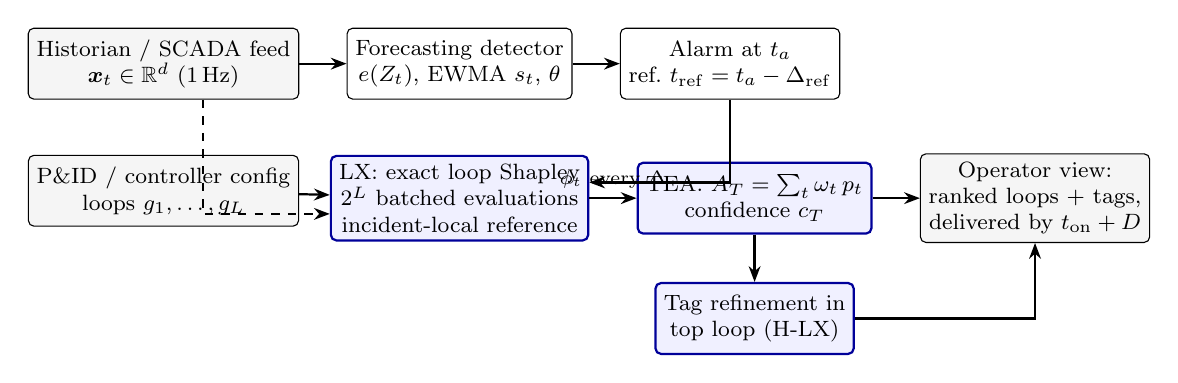
\begin{tikzpicture}[font=\footnotesize, node distance=4mm and 6mm,
  box/.style={draw, rounded corners=2pt, align=center, minimum height=9mm, inner sep=3pt, fill=white},
  data/.style={box, fill=black!4},
  ours/.style={box, draw=blue!60!black, fill=blue!6, thick},
  ar/.style={-{Stealth[length=2mm]}, thick}]
\node[data] (hist) {Historian / SCADA feed\\ $\bm x_t\in\mathbb R^d$ (1\,Hz)};
\node[box, right=of hist] (det) {Forecasting detector\\ $e(Z_t)$, EWMA $s_t$, $\theta$};
\node[box, right=of det] (alarm) {Alarm at $t_a$\\ ref.\ $t_{\mathrm{ref}}=t_a-\Delta_{\mathrm{ref}}$};
\node[data, below=7mm of hist] (pid) {P\&ID / controller config\\ loops $g_1,\dots,g_L$};
\node[ours, below=7mm of det] (lx) {\LX: exact loop Shapley\\ $2^L$ batched evaluations\\ incident-local reference};
\node[ours, right=of lx] (tea) {\TEA: $A_T=\sum_t\omega_t\,p_t$\\ confidence $c_T$};
\node[ours, below=6mm of tea] (ref) {Tag refinement in\\ top loop (H-\LX)};
\node[data, right=6mm of tea] (op) {Operator view:\\ ranked loops + tags,\\ delivered by $t_{\mathrm{on}}+D$};
\draw[ar] (hist) -- (det); \draw[ar] (det) -- (alarm);
\draw[ar] (pid) -- (lx); \draw[ar] (alarm.south) |- ($(lx.east)+(0,2mm)$);
\draw[ar] (lx) -- node[above,font=\scriptsize]{$\phi_t$ every $\Delta$} (tea);
\draw[ar] (tea) -- (op); \draw[ar] (tea) -- (ref); \draw[ar] (ref) -| (op);
\draw[ar, dashed] (hist.south) ++(5mm,0) |- ($(lx.west)+(0,-2mm)$);
\end{tikzpicture}}
\caption{Deadline-aware localization pipeline. Shaded blue: components proposed in this paper. The detector, the explainer and the delivery schedule together determine whether a correct localization reaches the operator before the deadline $D$.}\label{fig:arch}
\end{figure}

\subsection{Loop game with an incident-local reference}
At alarm time $t_a$ we fix a last-known-good reference time $t_{\mathrm{ref}}=t_a-\Delta_{\mathrm{ref}}$ ($\Delta_{\mathrm{ref}}=60$\,s by default; ablated in \cref{sec:ablation}). Let $Z_t=\bm x_{t-w:t}$ be the current segment and $R=\bm x_{t_{\mathrm{ref}}-w:t_{\mathrm{ref}}}$ the reference segment. For a coalition of loops $S\subseteq\mathcal G$ define the hybrid segment
\begin{equation}
[Z_t^S]_{\tau j}=\begin{cases}[Z_t]_{\tau j}& j\in\bigcup_{g\in S}g,\\ [R]_{\tau j}&\text{otherwise,}\end{cases}
\end{equation}
and the characteristic function $v_t(S)=e(Z^S_t)-e(Z^\emptyset_t)$.

The game asks how much of the current anomaly is explained by each loop's trajectory departing from its last known good trajectory, with all other loops restored to that state. This differs from the common interventional value function, which averages over a background drawn from training data \citep{lundberg2017shap,franco2026shats}. Background windows come from unrelated operating points (other setpoints, other plant states). Hybrid segments built from them are off-manifold for a forecaster and can themselves look anomalous. The incident-local reference keeps hybrids close to the operating point of the incident. We compare both choices empirically (\LX{} vs.\ \LX-bg).

\subsection{Exact loop Shapley values (\LX)}
The attribution of loop $g$ at time $t$ is its Shapley value \citep{shapley1953value}
\begin{equation}\label{eq:shapley}
\phi_t(g)=\sum_{S\subseteq\mathcal G\setminus\{g\}}\frac{|S|!\,(L-|S|-1)!}{L!}\bigl[v_t(S\cup\{g\})-v_t(S)\bigr].
\end{equation}
\begin{proposition}\label{prop:cost}
\LX{} requires exactly $2^L$ evaluations of $e(\cdot)$ per explanation, independent of the data and of $d$. It satisfies efficiency, $\sum_g\phi_t(g)=e(Z_t)-e(R)$. Since it is exact, it also satisfies the symmetry, dummy and additivity axioms.
\end{proposition}
\begin{proof}
All $2^L$ coalitions are evaluated once, and \cref{eq:shapley} is a fixed linear map of these values. The axioms are those of the Shapley value \citep{shapley1953value}, which hold because no sampling approximation is involved.
\end{proof}
The $2^L$ hybrid segments are evaluated in one batch. For $L\le 10$ this is at most 1024 forward passes of a small network. Explanation latency is therefore \emph{deterministic and known before deployment}, a property that sampling-based estimators lack. Exact Shapley values over $d$ tags would need $2^d$ evaluations ($d=57$ on HAI). Tag-level sampling estimators trade cost for variance \citep{castro2009sampling,strumbelj2014explaining}. Grouping by loops is an a priori union in the sense of \citet{owen1977unions}, as in ShaTS's multi-feature grouping \citep{franco2026shats}. The loop is also the unit in which ICS attacks are specified \citep{shin2021hai}. Finally, loop grouping encodes the sensor--actuator coupling that \citet{fung2024attributions} identify as a cause of attribution failure: a loop's SP, PV, CV and feedback enter or leave a coalition together.

\subsection{Temporal evidence accumulation (\TEA)}
An incident produces a sequence of explanations at times $t_a,t_a+\Delta,\dots$. Single-shot attributions are noisy. Worse, as the attack propagates through coupled loops, later residuals increasingly appear in loops that merely \emph{react}. Following \citet{fung2024attributions}, we expect the earliest windows to be most informative but not always reliable. \TEA{} therefore aggregates normalised positive attributions, weighted by severity:
\begin{equation}\label{eq:tea}
p_t(g)=\frac{\max(\phi_t(g),0)}{\sum_h\max(\phi_t(h),0)},\qquad A_T(g)=\sum_{t=t_a}^{T}\omega_t\,p_t(g),\qquad \omega_t=\log^+\!\frac{s_t}{\theta}+\varepsilon .
\end{equation}
The ranking published at $T$ sorts loops by $A_T$, with confidence margin $c_T=(A_T^{(1)}-A_T^{(2)})/\sum_g A_T(g)$, where $A_T^{(r)}$ is the $r$-th largest accumulated value. A deployment may publish as soon as $c_T\ge\gamma$, or at the deadline, whichever is first. \TEA{} is agnostic to the attribution method, so we apply it to every baseline as well.

\subsection{Tag refinement (H-\LX)}
Operators eventually need tags. Within the top-ranked loop $g^\star$ we compute exact Shapley values over its $|g^\star|$ tags. All other loops are held at their current values, so the game isolates within-loop responsibility; the cost is $2^{|g^\star|}$ evaluations ($\le 2^{12}$ on HAI).

\begin{algorithm}[t]
\caption{Deadline-aware localization for one incident}\label{alg:main}
\begin{algorithmic}[1]
\Require detector $(f,\sigma,\theta)$, loops $\mathcal G$, alarm time $t_a$, refresh $\Delta$, deadline $D$, threshold $\gamma$
\State $t_{\mathrm{ref}}\gets t_a-\Delta_{\mathrm{ref}}$;\ $R\gets\bm x_{t_{\mathrm{ref}}-w:t_{\mathrm{ref}}}$;\ $A\gets\bm 0\in\mathbb R^L$
\For{$t=t_a,\,t_a+\Delta,\dots$ \textbf{while} $t+\ell\le t_{\mathrm{on}}+D$}
  \State Build the $2^L$ hybrid segments $Z^S_t$; evaluate $e(\cdot)$ in one batch
  \State $\bm\phi_t\gets$ \cref{eq:shapley};\quad $A\gets A+\omega_t\,\bm p_t$ (\cref{eq:tea})
  \State Publish ranking $\operatorname{argsort}(-A)$ and margin $c$; \textbf{if} $c\ge\gamma$ \textbf{then} publish H-\LX{} tags for the top loop
\EndFor
\end{algorithmic}
\end{algorithm}

\section{Experimental design}\label{sec:setup}

\paragraph{Research questions}
RQ1: Which explainers localize the attacked loop at the alarm, and does control-loop structure matter beyond grouping per se? RQ2: How does accuracy evolve after the alarm, and does \TEA{} help? RQ3: Which explainers deliver correct localizations before a deadline once detection delay and latency are accounted for? RQ4: How robust are they to sensor noise and a decoy manipulation? RQ5: How much does a random window split inflate detection results? Hypotheses H1--H6 about \LX{} and \TEA{} and the decision rule (two-sided tests, Holm-corrected $p<0.05$ with the predicted sign) were fixed in the project's design document before the main runs (Supplementary Section~S1). The comparison with PI-CAX was added afterwards and is reported as a post hoc comparison; PI-CAX's design and constants were frozen before it was first run on either benchmark.

\subsection{Benchmarks}
\paragraph{HAI 21.03} HAI 21.03 \citep{shin2021hai} is a hardware-in-the-loop testbed coupling a boiler (P1), a turbine (P2) and a water-treatment process (P3) with a simulated power plant (P4). It records 79 tags at 1\,Hz: three normal training files (9.5 days) and five test files with 50 attacks (25 single, 25 combined). Its documentation lists the target controller(s) and manipulated points of every attack.
\begin{itemize}
\item \emph{Ground truth.} We transcribed this table and matched every entry to the label runs in the data (all start times agree within 2\,min); three point names were mapped to their 21.03 columns. An independent transcription of the same table, produced separately within the project, agrees on the target loops and points of \gtcrossAgree{} of \gtcrossN{} attacks. The one disagreement (A401) is a row continuing across a page break; we keep its second scenario, as for every A4xx attack, and excluding A401 changes no reported HR@1 by more than \aFourZeroOneMaxDiff.
\item \emph{Loop map.} Tags were assigned to loop groups from the tag descriptions before any test data was examined (Supplementary Section~S3). Twenty-two tags are constant in normal training and removed, leaving $d=\HAId$ tags in $L=\HAIL$ groups.
\item \emph{Hidden setpoints.} Manipulated setpoints are largely invisible in the recorded data: of \spN{} (attack, setpoint-tag) targets, \spConstant{} are exactly constant during the attack and only \spVisible{} vary beyond their range in the preceding 10\,min. Tag-level localization of those points is impossible from the data; loop-level localization is not.
\end{itemize}

\paragraph{PCL-Sim} The simulator models a supply tank, a transfer valve, a heated tank, a centrifugal pump and a discharge valve under five PI loops (tank-1 level, transfer flow, tank-2 level via pump speed, tank-2 temperature, discharge pressure), with actuator dynamics, hydraulic and thermal coupling, sensor noise, random-walk disturbances and an operator schedule that changes setpoints every 15--45\,min. It exposes $d=22$ tags in $L=6$ groups (five loops and a disturbance group). Seven attack primitives mirror HAI (SP, CV offset, PV bias, PV freeze, CV+PV-freeze, SP+PV-freeze, short CV pulses), applied to each loop at two magnitudes and four test seeds, for \SimNattacks{} one-hour episodes. Controllers and historian see the manipulated values while the true state is integrated separately; the hazard deadline $D^{\mathrm{haz}}$ is the time to the first violation of a safety limit (overflow or dry-run, temperature $>85\,^\circ$C, pressure $>8.5$\,bar). \SimNhaz{} attacks are hazardous (median $D^{\mathrm{haz}}=\SimHazMedian$\,s, range \SimHazMin--\SimHazMax\,s). Twelve 6-hour normal runs with disjoint seeds are used for training and validation.

\subsection{Detectors and leakage control}
Four forecaster families are trained on normal data only, with three seeds each and window $w=32$: a linear autoregressive model (closed-form ridge), an MLP, a dilated 1D-CNN \citep[cf.][]{kravchik2018cnn} and a GRU. Normal files are split chronologically (80\,\% train, 20\,\% validation); standardisation comes from training data, and $\sigma_j$ and $\theta$ ($q=0.999$, $\alpha=0.1$) from validation data only. No test labels, files or seeds are used for any fitting or hyperparameter choice.

\subsection{Explainers}
All explainers attribute the same score $e(Z_t)$; tag-level attributions are summed per loop.
\begin{itemize}
\item \emph{Tag-level baselines:} raw squared residuals (RE; the ``MSE'' ranking of \citealp{fung2024attributions}), saliency (SM; \citealp{simonyan2014saliency}), integrated gradients from the reference (IG, 32 steps; \citealp{sundararajan2017ig}), KernelSHAP \citep{lundberg2017shap} and LIME \citep{ribeiro2016lime} with $2^L$ (``eq'') or 1024 samples, and the ensemble of \citet{fung2024attributions} (RE + SM + LIME in place of LEMNA, $\beta=2.5$ for actuators).
\item \emph{Loop-structured:} \LX, \LX-bg (\LX{} with an interventional background of 8 training windows) and PI-CAX (\cref{sec:picax}).
\item \emph{Structure controls:} exact Shapley over $L$ correlation clusters (CLX) or a random partition with the loop group sizes (RPX).
\item \emph{ShaTS-sensor} \citep{franco2026shats}, with $m=20\,|G|$ coalitions per group; its cost ($\approx2\cdot20\,d^2$ evaluations) restricts it to two detectors at the alarm.
\end{itemize}
Every method is run single-shot and with \TEA.

\subsection{Protocol, metrics and statistics}
Following \citet{fung2024attributions}, explanations are computed at a best-guess timing (oracle window starting at onset) and at practical timing: from the first alarm every $\Delta=5$\,s for 180\,s.
\begin{itemize}
\item \emph{Detection:} point-wise precision, recall and F1 without point adjustment \citep{kim2022rigorous}, event recall (alarm within the attack or 60\,s after it), median delay and false alarms per hour.
\item \emph{Localization:} HR@$k$ (a target loop among the top $k$) and normalised rank, against a uniformly random ranking as chance reference.
\item \emph{Faithfulness:} deletion AUC, restoring loops in ranked order to the training mean (lower is better).
\item \emph{Stability:} top-$k$ agreement between consecutive explanations, and Jaccard agreement under Gaussian input noise ($\sigma=0.1$).
\item \emph{Cost and timeliness:} median wall-clock latency on one CPU thread, detector evaluations per explanation, DCL@$k(D)$ and the in-time rate with $t_{\mathrm{act}}=30$\,s.
\end{itemize}
The unit of analysis is the attack: seeds are averaged per (attack, detector), and these pairs are the paired units. We report means with 95\,\% bootstrap confidence intervals and test with a Friedman omnibus and two-sided Wilcoxon signed-rank tests against a reference configuration, Holm-corrected \citep{demsar2006statistical,holm1979simple}, with matched-pairs rank-biserial effect sizes $r_{\mathrm{rb}}$. Experiments ran with Python~3.13 and PyTorch~2.15 on an \CPUmodel{}; latencies use one thread (\texttt{torch.set\_num\_threads(1)}).

\section{Results}\label{sec:results}

\subsection{Detection}
On HAI, the four detectors detect 89--92\,\% of the 50 attacks at 0.34--0.42 false alarms per hour, with median delays of 6--15\,s (\cref{tab:detection}). On PCL-Sim, event recall is 76--96\,\%; point-wise recall is low because the PI controllers partly compensate the manipulations. In ten HAI attacks the score crosses $\theta$ 1--4\,s before the labelled onset, which suggests that documented onsets lag slightly; we keep the documented labels. Localization is evaluated on detected attacks (\nhaitesthrOnealarmZero{} (attack, detector) units on HAI, \nsimtesthrOnealarmZero{} on PCL-Sim); deadline metrics count missed detections as failures.

\begin{table}[t]
\centering\scriptsize
\caption{Detection performance (mean$\pm$sd over 3 seeds; no point adjustment). Event recall: alarm within the attack or 60\,s after it. FA/h: false-alarm runs per hour of attack-free data.}\label{tab:detection}
\resizebox{\linewidth}{!}{%
\begin{tabular}{@{}llcccccc@{}}
\toprule
Data & Detector & P & R & F1 & Event rec. & Delay [s] & FA/h\\
\midrule
PCL-Sim & Linear & 0.79 & 0.17 & 0.28 & 0.96 & 6 & 1.38\\
 & MLP & 0.81$\pm$0.06 & 0.07$\pm$0.04 & 0.13$\pm$0.07 & 0.76$\pm$0.03 & 226$\pm$176 & 0.31$\pm$0.03\\
 & CNN & 0.83$\pm$0.03 & 0.19$\pm$0.02 & 0.31$\pm$0.02 & 0.89$\pm$0.00 & 46$\pm$38 & 0.96$\pm$0.06\\
 & GRU & 0.77$\pm$0.02 & 0.42$\pm$0.01 & 0.54$\pm$0.01 & 0.93$\pm$0.00 & 7$\pm$1 & 0.89$\pm$0.05\\
\midrule
HAI 21.03 & Linear & 0.79$\pm$0.00 & 0.60$\pm$0.00 & 0.68$\pm$0.00 & 0.92 & 6 & 0.42$\pm$0.03\\
 & MLP & 0.75$\pm$0.01 & 0.50$\pm$0.02 & 0.60$\pm$0.02 & 0.90 & 15$\pm$1 & 0.36$\pm$0.04\\
 & CNN & 0.74$\pm$0.01 & 0.48$\pm$0.01 & 0.58$\pm$0.01 & 0.89$\pm$0.01 & 14$\pm$0 & 0.34$\pm$0.01\\
 & GRU & 0.78$\pm$0.00 & 0.55$\pm$0.00 & 0.65$\pm$0.00 & 0.90 & 14$\pm$1 & 0.36$\pm$0.02\\
\bottomrule
\end{tabular}}
\end{table}


\subsection{Localization at the alarm (RQ1)}
\Cref{tab:loc_hai,tab:loc_sim} report loop localization for all configurations.
\begin{itemize}
\item \emph{PI-CAX is the most accurate explainer.} It ranks the attacked loop first in \lochaiPICAXalarmZerosinglehrOne{} of detected attacks on HAI and \locsimPICAXalarmZerosinglehrOne{} on PCL-Sim, significantly better than every other configuration (Holm $p\pctesthaialarmmaxp$ on HAI and $p\pctestsimalarmmaxp$ on PCL-Sim, $n=\pctesthaialarmn$ and \pctestsimalarmn).
\item \emph{Among score attributions,} \LX{} is the most accurate on HAI (\lochaiLXalarmZerosinglehrOne; IG \lochaiIGalarmZerosinglehrOne, Holm $p=\phaitesthrOnealarmZeroIGtea$), whereas on PCL-Sim most score attributions lie within two points of each other (\LX{} \locsimLXalarmZerosinglehrOne, \LX-bg \locsimLXbgalarmZerosinglehrOne). H1 is therefore only partially supported.
\item \emph{Chance and structure.} A random ranking would rank a target loop first in \chancehaihrOne{} of the same units on both benchmarks (HAI \chancehaihrOne, PCL-Sim \chancesimhrOne). Exact Shapley values over correlation clusters (CLX) or random groups of the loop sizes (RPX) reach only 0.45/0.25 on HAI and 0.27/0.54 on PCL-Sim (all Holm $p<10^{-10}$ against \LX), so the gain of loop attribution comes from control structure, not grouping per se (H4 supported).
\item \emph{Best-guess timing} \citep{fung2024attributions} does not help: on HAI it is worse than practical timing for every method except saliency, which is unchanged (\LX{} \lochaiLXbestguesssinglehrOne), because many manipulations take tens of seconds to affect the process.
\end{itemize}

\begin{table}[t]
\centering\scriptsize
\caption{Loop localization on HAI 21.03 (pooled over 4 detectors; mean over attacks, seeds averaged). Bold: best in column. Single-shot unless marked \TEA.}\label{tab:loc_hai}
\resizebox{\linewidth}{!}{%
\begin{tabular}{@{}lcccccccc@{}}
\toprule
& \multicolumn{6}{c}{HR@1} & HR@3 & nRank\\\cmidrule(lr){2-7}\cmidrule(lr){8-8}\cmidrule(lr){9-9} Method & best-guess & alarm & +60\,s & +60\,s\,\TEA & +180\,s & +180\,s\,\TEA & +60\,s\,\TEA & +60\,s\,\TEA\\
\midrule
RE & 0.49 & 0.71 & 0.48 & 0.61 & \textbf{0.35} & 0.57 & 0.89 & 0.09\\
SM & 0.43 & 0.43 & 0.32 & 0.44 & 0.22 & 0.44 & 0.67 & 0.27\\
IG & 0.50 & 0.75 & 0.56 & \textbf{0.72} & 0.33 & 0.70 & 0.93 & \textbf{0.06}\\
KernelSHAP-eq & 0.47 & 0.70 & 0.50 & 0.64 & 0.22 & 0.60 & 0.90 & 0.09\\
KernelSHAP-1024 & 0.48 & 0.74 & 0.51 & 0.69 & 0.28 & 0.65 & 0.92 & 0.07\\
LIME-eq & 0.49 & 0.75 & 0.55 & 0.70 & 0.26 & 0.66 & 0.93 & 0.07\\
LIME-1024 & 0.49 & 0.76 & 0.56 & 0.69 & 0.31 & 0.66 & 0.93 & 0.07\\
Fung ens. & \textbf{0.60} & 0.76 & 0.56 & \textbf{0.72} & 0.34 & \textbf{0.71} & 0.92 & 0.07\\
CLX (clusters) & 0.31 & 0.45 & 0.39 & 0.38 & 0.20 & 0.38 & 0.79 & 0.18\\
RPX (random) & 0.17 & 0.25 & 0.19 & 0.21 & 0.16 & 0.17 & 0.68 & 0.26\\
\LX-bg & 0.55 & 0.74 & 0.58 & 0.71 & 0.31 & 0.65 & \textbf{0.94} & \textbf{0.06}\\
\textbf{\LX{} (ours)} & 0.47 & \textbf{0.79} & \textbf{0.60} & 0.70 & 0.30 & 0.64 & \textbf{0.94} & \textbf{0.06}\\
\bottomrule
\end{tabular}}
\end{table}

\begin{table}[t]
\centering\scriptsize
\caption{Loop localization on PCL-Sim (pooled over 4 detectors; mean over attacks, seeds averaged). Bold: best in column. Single-shot unless marked \TEA.}\label{tab:loc_sim}
\resizebox{\linewidth}{!}{%
\begin{tabular}{@{}lcccccccc@{}}
\toprule
& \multicolumn{6}{c}{HR@1} & HR@3 & nRank\\\cmidrule(lr){2-7}\cmidrule(lr){8-8}\cmidrule(lr){9-9} Method & best-guess & alarm & +60\,s & +60\,s\,\TEA & +180\,s & +180\,s\,\TEA & +60\,s\,\TEA & +60\,s\,\TEA\\
\midrule
RE & 0.43 & 0.86 & 0.44 & 0.80 & 0.41 & 0.80 & 0.96 & 0.07\\
SM & 0.44 & 0.65 & 0.43 & 0.70 & 0.40 & 0.69 & 0.95 & 0.10\\
IG & \textbf{0.68} & 0.86 & 0.66 & 0.84 & 0.55 & 0.83 & 0.96 & 0.06\\
KernelSHAP-eq & 0.46 & 0.80 & 0.47 & 0.71 & 0.40 & 0.69 & 0.90 & 0.13\\
KernelSHAP-1024 & 0.50 & 0.84 & 0.50 & 0.80 & 0.43 & 0.77 & 0.93 & 0.09\\
LIME-eq & 0.42 & 0.82 & 0.46 & 0.72 & 0.40 & 0.70 & 0.91 & 0.12\\
LIME-1024 & 0.50 & 0.85 & 0.52 & 0.82 & 0.45 & 0.81 & 0.95 & 0.07\\
Fung ens. & 0.48 & 0.87 & 0.49 & 0.82 & 0.45 & 0.82 & 0.97 & 0.06\\
PI-CAX & -- & \textbf{0.89} & \textbf{0.79} & \textbf{0.87} & \textbf{0.72} & \textbf{0.87} & \textbf{0.99} & \textbf{0.04}\\
CLX (clusters) & 0.12 & 0.27 & 0.16 & 0.23 & 0.14 & 0.23 & 0.78 & 0.31\\
RPX (random) & 0.35 & 0.54 & 0.35 & 0.58 & 0.32 & 0.58 & 0.90 & 0.16\\
\LX-bg & 0.54 & 0.87 & 0.60 & 0.85 & 0.50 & 0.83 & 0.96 & 0.06\\
\LX & 0.57 & 0.85 & 0.53 & 0.82 & 0.46 & 0.80 & 0.95 & 0.07\\
\bottomrule
\end{tabular}}
\end{table}


\subsection{After the alarm: propagation and temporal accumulation (RQ2)}
Single-shot score attributions degrade quickly after the alarm, for every method (\cref{fig:overtime}). On HAI, \LX{} falls from \lochaiLXalarmZerosinglehrOne{} at the alarm to \lochaiLXalarmSixZerosinglehrOne{} after 60\,s and \lochaiLXalarmOneEightZerosinglehrOne{} after 180\,s; on PCL-Sim from \locsimLXalarmZerosinglehrOne{} to \locsimLXalarmSixZerosinglehrOne{} and \locsimLXalarmOneEightZerosinglehrOne. Once controllers react, the largest residuals move to loops that compensate for the manipulated one, which adds a mechanism to the timing effect of \citet{fung2024attributions}.
\begin{itemize}
\item \emph{\TEA{} recovers part of the loss for every method} (H2 supported). \LX+\TEA{} reaches \lochaiLXalarmSixZeroteahrOne{} (HAI) and \locsimLXalarmSixZeroteahrOne{} (PCL-Sim) at 60\,s (Holm $p=\phaitesthrOnealarmSixZeroLXsingle$ and $p=\psimtesthrOnealarmSixZeroLXsingle$ against single-shot), and single-shot top-1 outputs that change between consecutive explanations in 12--48\,\% of cases become 95--100\,\% consistent (\cref{tab:quality}). With \TEA, the leading score attributions are within a few points of each other: on HAI \LX{} is not significantly different from IG, \LX-bg, the Fung ensemble, LIME-1024 or KernelSHAP-1024; on PCL-Sim IG and \LX-bg are slightly but significantly better (Supplementary Table~S2).
\item \emph{PI-CAX degrades far less.} Single-shot, it still reaches \lochaiPICAXalarmSixZerosinglehrOne{} (HAI) and \locsimPICAXalarmSixZerosinglehrOne{} (PCL-Sim) at 60\,s; with \TEA, \lochaiPICAXalarmSixZeroteahrOne{} and \locsimPICAXalarmSixZeroteahrOne, significantly better than every other configuration (Holm $p\pctesthaisixtymaxp$ and $p\pctestsimsixtymaxp$). With \TEA, the attacked loop is among PI-CAX's top three in \lochaiPICAXalarmSixZeroteahrThree{} and \locsimPICAXalarmSixZeroteahrThree{} of cases.
\end{itemize}

\begin{figure}[t]
\centering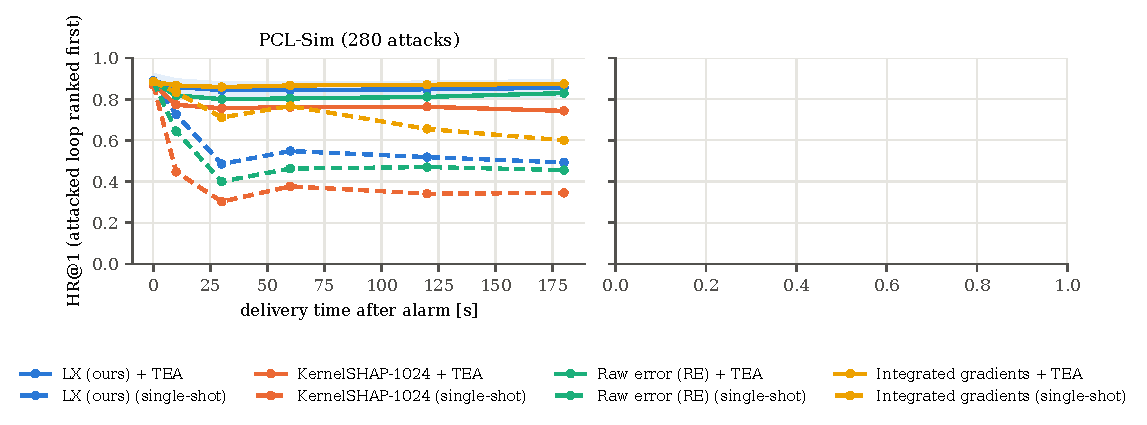
\includegraphics[width=\linewidth]{figures/hr1_over_time.pdf}
\caption{Top-1 loop localization versus delivery time after the alarm (solid: with \TEA; dashed: single-shot; band: 95\,\% bootstrap CI for \LX+\TEA). Score attributions decay as the attack propagates through coupled loops; PI-CAX decays least.}\label{fig:overtime}
\end{figure}


\subsection{Why the physical prior works}
\Cref{tab:pcab} switches PI-CAX's components off one at a time (seed 0, all four detectors). Removing the persistence--oscillation decoupling reduces it to the level of the score attributions (HAI: \pcabhaiNoCausalalarm{} at the alarm and \pcabhaiNoCausalsingle{} single-shot at 60\,s). Removing the precision weighting and loop gating, the operating envelope or the counterfactual check changes accuracy by at most 0.04. The advantage therefore comes from one physical hypothesis: the manipulated loop departs \emph{persistently} from its normal cross-loop relations, while compensating loops \emph{oscillate}. Score attributions cannot express this distinction, because they only ask how much each loop contributes to the current score.

\begin{table}[t]
\centering\scriptsize
\caption{PI-CAX component ablation: loop HR@1 (single-shot at the alarm / single-shot at +60\,s / +60\,s with \TEA; seed 0, four detectors pooled).}\label{tab:pcab}
\begin{tabular}{@{}lcc@{}}
\toprule
Configuration & HAI 21.03 & PCL-Sim\\
\midrule
Full PI-CAX & \pcabhaiFullalarm{} / \pcabhaiFullsingle{} / \pcabhaiFulltea & \pcabsimFullalarm{} / \pcabsimFullsingle{} / \pcabsimFulltea\\
-- persistence/oscillation decoupling & \pcabhaiNoCausalalarm{} / \pcabhaiNoCausalsingle{} / \pcabhaiNoCausaltea & \pcabsimNoCausalalarm{} / \pcabsimNoCausalsingle{} / \pcabsimNoCausaltea\\
-- precision weighting and loop gating & \pcabhaiNoManifoldalarm{} / \pcabhaiNoManifoldsingle{} / \pcabhaiNoManifoldtea & \pcabsimNoManifoldalarm{} / \pcabsimNoManifoldsingle{} / \pcabsimNoManifoldtea\\
-- operating envelope & \pcabhaiNoEnvelopealarm{} / \pcabhaiNoEnvelopesingle{} / \pcabhaiNoEnvelopetea & \pcabsimNoEnvelopealarm{} / \pcabsimNoEnvelopesingle{} / \pcabsimNoEnvelopetea\\
-- counterfactual check & \pcabhaiNoTieralarm{} / \pcabhaiNoTiersingle{} / \pcabhaiNoTiertea & \pcabsimNoTieralarm{} / \pcabsimNoTiersingle{} / \pcabsimNoTiertea\\
none (smoothed residuals only) & \pcabhaiNonealarm{} / \pcabhaiNonesingle{} / \pcabhaiNonetea & \pcabsimNonealarm{} / \pcabsimNonesingle{} / \pcabsimNonetea\\
\bottomrule
\end{tabular}
\end{table}

\paragraph{Hard-to-explain attacks} \Cref{tab:strata} stratifies HAI by the type of manipulated variable, read from the target-controller code of the official attack table (strata of 3--\stratcombn{} attacks; descriptive only). Controller-output (CV) attacks move a recorded actuator and are localized well by most methods (0.79 at the alarm for IG, KernelSHAP-1024, \LX-bg and \LX). Setpoint (SP) attacks are the hardest for score attributions: the setpoint is largely invisible in the data, and every score attribution falls to \stratSPteamin--\stratSPteamax{} at 60\,s even with \TEA. PI-CAX localizes them in \stratSPPICAXtea{} of cases, plausibly because a hidden setpoint change produces exactly the persistent PV/CV departure it looks for. Its weakest stratum is SP attacks combined with a PV spoof (\stratSPPVPICAXtea{} at 60\,s, $n=\stratSPPVn$), possibly because the spoofed PV hides the persistent departure.

\begin{table}[htbp]
\centering\scriptsize
\caption{HAI 21.03 loop HR@1 by manipulated variable type, read from the target-controller code of the official attack table (attacks detected by at least one detector; single-shot at the alarm / +60\,s with \TEA; pooled over 4 detectors). Strata are small; descriptive only.}\label{tab:strata}
\resizebox{\linewidth}{!}{%
\begin{tabular}{@{}lccccccc@{}}
\toprule
Manipulated variable & attacks & RE & IG & KernelSHAP-1024 & \LX-bg & \LX & PI-CAX\\
\midrule
SP only & 8 & 0.69 / 0.38 & 0.66 / 0.52 & 0.66 / 0.46 & 0.65 / 0.47 & 0.73 / 0.46 & 0.93 / 0.98\\
SP + PV spoof & 4 & 0.50 / 0.31 & 0.56 / 0.65 & 0.58 / 0.60 & 0.65 / 0.62 & 0.71 / 0.62 & 0.75 / 0.52\\
CV only & 8 & 0.69 / 0.74 & 0.79 / 0.79 & 0.79 / 0.78 & 0.79 / 0.84 & 0.79 / 0.79 & 0.99 / 0.98\\
CV + PV spoof & 3 & 0.94 / 0.89 & 0.97 / 0.92 & 0.92 / 0.78 & 0.97 / 0.94 & 1.00 / 0.89 & 1.00 / 1.00\\
combined (2 scenarios) & 23 & 0.73 / 0.66 & 0.77 / 0.76 & 0.75 / 0.74 & 0.74 / 0.73 & 0.80 / 0.74 & 0.93 / 0.96\\
\bottomrule
\end{tabular}}
\end{table}


\subsection{Deadlines, latency and cost (RQ3)}
\Cref{tab:deadline_hai,tab:deadline_sim} and \cref{fig:dcl} account for detection delay, explainer latency and the correctness of the delivered explanation.
\begin{itemize}
\item \emph{HAI.} DCL@1 at $D=60$\,s is \dclhaiPICAXdclfixedSixZerotea{} for PI-CAX+\TEA{} against \dclhaiLXdclfixedSixZerotea{} for \LX+\TEA{} and at most \dclhaiIGdclfixedSixZerotea{} for any other configuration (Holm $p\pctesthaidclmaxp$, $n=\pctesthaidcln$). It is bounded by event recall, so PI-CAX delivers a correct loop for most detected attacks within a minute of onset. No score attribution differs significantly from \LX{} in DCL@1 at 60\,s (H3 not supported for DCL).
\item \emph{PCL-Sim.} The correct loop is ranked first before the hazard deadline minus a 30\,s action reserve in \dclsimLXdclhazhztea{} (\LX+\TEA), \dclsimPICAXdclhazhztea{} (PI-CAX+\TEA) and \dclsimIGdclhazhztea{} (IG+\TEA) of hazardous cases. No explainer improves this rate materially, because the failures are dominated by detection: of the \intimeFail{} failing (attack, detector, seed) cases of \LX+\TEA, \intimeFailUndelivered{} (\intimeFailUndeliveredPct\,\%) were detected too late for any explanation to be delivered. Conditional on delivery, the top-ranked loop is correct in \intimeDeliveredLX{} (\LX), \intimeDeliveredPICAX{} (PI-CAX) and \intimeDeliveredIG{} (IG) of cases.
\item \emph{Latency.} \LX{} costs $2^L$ evaluations per explanation (512 on HAI, 64 on PCL-Sim), i.e.\ \latsimLXlinear--\latsimLXcnn\,ms on PCL-Sim and \lathaiLXlinear--\lathaiLXcnn\,ms on HAI on one thread (\cref{tab:latency}); PI-CAX needs 16 evaluations (median 1.4--1.7\,ms during the runs, \cref{tab:deadline_hai,tab:deadline_sim}). Both are deterministic and need no gradients; IG is cheaper than \LX{} but requires gradient access.
\item \emph{Slower hardware.} We did not measure on embedded devices. Multiplying every measured latency by an assumed factor of 10 or 100 changes DCL@1 at $D=30$\,s by at most 0.04 for all configurations except \LX-bg on HAI (4096 evaluations), which drops from \slowhaixoneLXbgthirty{} to \slowhaixhundredLXbgthirty. At these model sizes, latency is not the binding constraint; detection delay is.
\item \emph{ShaTS-sensor} needs $\approx\!2\cdot20\,d^2$ evaluations ($\evalshaiShaTS$ on HAI), \lathaiShaTScnn\,s for the CNN. At the alarm on HAI it localizes \shatshaicnnHR{} of attacks against \shatshaicnnLXHR{} for \LX{} on the same incidents (CNN, seed 0, $n=\shatshaicnnN$; linear: \shatshailinearHR{} vs.\ \shatshailinearLXHR), at roughly 250--280 times the cost.
\end{itemize}

\begin{figure}[t]
\centering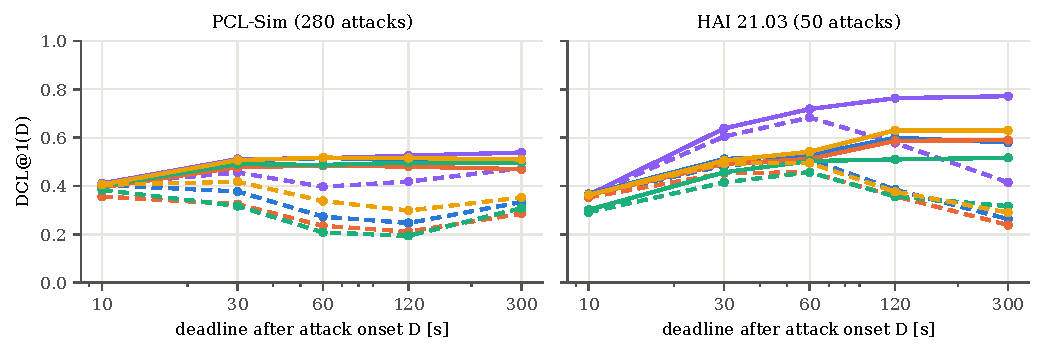
\includegraphics[width=\linewidth]{figures/dcl.pdf}
\caption{Deadline-conditioned localization DCL@1($D$) (colours as in \cref{fig:overtime}; solid: \TEA; dashed: single-shot). Missed detections and undelivered explanations count as failures, so curves are bounded by event recall.}\label{fig:dcl}
\end{figure}

\begin{table}[t]
\centering\scriptsize
\caption{Deadline-conditioned localization on HAI 21.03 (T = with \TEA). Latency: median measured per explanation during the runs (1 thread, pooled over detectors); Evals: detector evaluations per explanation.}\label{tab:deadline_hai}
\resizebox{\linewidth}{!}{%
\begin{tabular}{@{}lccccccc@{}}
\toprule
Method & \multicolumn{4}{c}{DCL@1($D$)} & DCL@3 & Lat.\,[ms] & Evals\\ & 30\,s\,T & 60\,s & 60\,s\,T & 120\,s\,T & 60\,s\,T & & \\
\midrule
RE & 0.46 & 0.46 & 0.50 & 0.51 & 0.68 & 0.5 & 1\\
SM & 0.32 & 0.31 & 0.32 & 0.39 & 0.49 & 1.0 & 1\\
IG & 0.51 & 0.49 & 0.54 & 0.63 & 0.68 & 3.4 & 32\\
KernelSHAP-eq & 0.47 & 0.41 & 0.48 & 0.55 & 0.67 & 20.4 & 512\\
KernelSHAP-1024 & 0.49 & 0.46 & 0.51 & 0.59 & 0.68 & 40.9 & 1024\\
LIME-eq & 0.50 & 0.48 & 0.52 & 0.60 & 0.68 & 38.1 & 512\\
LIME-1024 & 0.51 & 0.50 & 0.52 & 0.60 & 0.69 & 85.9 & 1024\\
Fung ens. & 0.54 & 0.51 & 0.54 & 0.62 & 0.72 & 43.8 & 514\\
PI-CAX & \textbf{0.64} & \textbf{0.68} & \textbf{0.72} & \textbf{0.76} & \textbf{0.78} & 1.7 & 16\\
CLX (clusters) & 0.30 & 0.34 & 0.32 & 0.34 & 0.61 & 14.2 & 512\\
RPX (random) & 0.16 & 0.17 & 0.19 & 0.17 & 0.52 & 13.0 & 512\\
\LX-bg & 0.51 & 0.51 & 0.53 & 0.60 & 0.70 & 200.2 & 4096\\
\LX & 0.51 & 0.51 & 0.53 & 0.60 & 0.70 & 28.2 & 512\\
\bottomrule
\end{tabular}}
\end{table}

\begin{table}[t]
\centering\scriptsize
\caption{Deadline-conditioned localization on PCL-Sim (T = with \TEA). Latency: median measured per explanation during the runs (1 thread, pooled over detectors); Evals: detector evaluations per explanation. In-time: hazard deadline minus a 30\,s operator reserve, hazardous attacks only.}\label{tab:deadline_sim}
\resizebox{\linewidth}{!}{%
\begin{tabular}{@{}lcccccccccc@{}}
\toprule
Method & \multicolumn{4}{c}{DCL@1($D$)} & DCL@3 & \multicolumn{2}{c}{In-time@1} & In-time@3 & Lat.\,[ms] & Evals\\ & 30\,s\,T & 60\,s & 60\,s\,T & 120\,s\,T & 60\,s\,T & single & T & T & & \\
\midrule
RE & 0.49 & 0.21 & 0.49 & 0.50 & \textbf{0.53} & 0.17 & 0.41 & \textbf{0.54} & 0.3 & 1\\
SM & 0.47 & 0.21 & 0.46 & 0.47 & \textbf{0.53} & 0.19 & 0.40 & \textbf{0.54} & 0.8 & 1\\
IG & \textbf{0.51} & \textbf{0.34} & \textbf{0.52} & \textbf{0.52} & \textbf{0.53} & \textbf{0.33} & \textbf{0.50} & \textbf{0.54} & 2.2 & 32\\
KernelSHAP-eq & 0.40 & 0.23 & 0.40 & 0.40 & 0.48 & 0.25 & 0.40 & 0.51 & 2.4 & 64\\
KernelSHAP-1024 & 0.48 & 0.24 & 0.48 & 0.48 & 0.52 & 0.22 & 0.43 & 0.51 & 24.2 & 1024\\
LIME-eq & 0.42 & 0.21 & 0.42 & 0.42 & 0.50 & 0.20 & 0.38 & 0.48 & 1.8 & 64\\
LIME-1024 & 0.50 & 0.24 & 0.50 & 0.50 & \textbf{0.53} & 0.22 & 0.46 & 0.52 & 15.4 & 1024\\
Fung ens. & 0.50 & 0.23 & 0.50 & 0.50 & \textbf{0.53} & 0.21 & 0.44 & \textbf{0.54} & 3.2 & 66\\
CLX (clusters) & 0.10 & 0.09 & 0.10 & 0.10 & 0.41 & 0.10 & 0.14 & 0.38 & 1.6 & 64\\
RPX (random) & 0.32 & 0.17 & 0.33 & 0.35 & 0.51 & 0.17 & 0.29 & 0.50 & 1.5 & 64\\
\LX-bg & \textbf{0.51} & 0.28 & \textbf{0.52} & \textbf{0.52} & \textbf{0.53} & 0.29 & 0.49 & \textbf{0.54} & 7.3 & 512\\
\textbf{\LX{} (ours)} & \textbf{0.51} & 0.27 & \textbf{0.52} & 0.51 & \textbf{0.53} & 0.28 & 0.48 & 0.53 & 1.6 & 64\\
\bottomrule
\end{tabular}}
\end{table}

\begin{table}[t]
\centering\tiny
\caption{Explanation latency on one CPU thread of an otherwise idle machine (median over 10 incidents $\times$ 5 repetitions, ms; ShaTS: 2 incidents, 1 repetition). Evals: detector evaluations per explanation.}\label{tab:latency}
\resizebox{\linewidth}{!}{%
\begin{tabular}{@{}llrrrrr@{}}
\toprule
Data & Method & Evals & Linear & MLP & CNN & GRU\\
\midrule
\bottomrule
\end{tabular}}
\end{table}


\subsection{Explanation quality beyond accuracy}
\Cref{tab:quality} reports further properties.
\begin{itemize}
\item \emph{Faithfulness.} Deletion AUCs at the alarm are similar for all accurate methods (0.16--0.22), including PI-CAX; saliency and the structure controls are worse.
\item \emph{Stability under input noise.} On HAI, PI-CAX's single explanations are the most sensitive to Gaussian input perturbation (top-3 Jaccard \qhaiPICAXnoise{} on HAI, against \qhaiLXnoise{} for \LX{} and 0.70 for KernelSHAP-1024), because its persistence statistics use only ten samples. Exact attributions are also less stable than fixed-seed sampling estimators. \TEA{} mitigates both in operation.
\item \emph{Tags.} Within the top loop, H-\LX{} ranks a manipulated tag first in \qhaiLXtagone{} (HAI) and \qsimLXtagone{} (PCL-Sim) of attacks; PI-CAX's tag ranking reaches \qhaiPICAXtagone{} and \qsimPICAXtagone{}, the best of all methods.
\end{itemize}

\begin{table}[t]
\centering\scriptsize
\caption{Explanation quality. Temporal agreement: share of consecutive explanations (5\,s apart, first 120\,s) with the same top-1 loop. Noise Jaccard: top-3 overlap under Gaussian input noise ($\sigma=0.1$) at alarm and +60\,s. Deletion: area under the normalised score curve when loops are restored to the training mean in ranked order (lower is better), at the alarm. Tag HR@$k$: rank of a manipulated tag among all tags at the alarm (for \LX: H-\LX{} refinement); HAI excludes P2 setpoint targets that are invisible in the data.}\label{tab:quality}
\resizebox{\linewidth}{!}{%
\begin{tabular}{@{}llcccccc@{}}
\toprule
Data & Method & \multicolumn{2}{c}{Temporal top-1 agr.} & Noise Jacc.@3 & Deletion$\downarrow$ & Tag HR@1 & Tag HR@3\\ & & single & \TEA & & & & \\
\midrule
PCL-Sim & RE & 0.53 & 0.99 & 0.49 & 0.18 & 0.38 & \textbf{0.76}\\
 & SM & 0.52 & 0.99 & 0.53 & 0.28 & 0.20 & 0.53\\
 & IG & 0.71 & \textbf{1.00} & 0.53 & 0.18 & 0.44 & 0.74\\
 & KernelSHAP-eq & \textbf{0.77} & 0.99 & 0.71 & 0.19 & 0.43 & 0.69\\
 & KernelSHAP-1024 & 0.74 & 0.99 & 0.62 & 0.18 & 0.44 & 0.73\\
 & LIME-eq & 0.74 & 0.99 & 0.71 & 0.21 & 0.41 & 0.69\\
 & LIME-1024 & 0.70 & 0.99 & 0.59 & 0.20 & 0.44 & 0.73\\
 & Fung ens. & 0.59 & 0.99 & 0.60 & \textbf{0.17} & 0.28 & 0.75\\
 & CLX (clusters) & 0.61 & 0.99 & 0.64 & 0.34 & 0.05 & 0.27\\
 & RPX (random) & 0.63 & 0.98 & \textbf{0.76} & 0.26 & 0.00 & 0.08\\
 & \LX-bg & 0.66 & 0.99 & 0.55 & 0.22 & -- & --\\
 & \textbf{\LX{} (ours)} (H-\LX) & 0.64 & 0.99 & 0.51 & 0.21 & \textbf{0.45} & \textbf{0.76}\\
\midrule
HAI 21.03 & RE & 0.58 & 0.95 & 0.59 & 0.18 & 0.23 & 0.40\\
 & SM & 0.62 & 0.95 & 0.44 & 0.45 & 0.10 & 0.34\\
 & IG & 0.67 & \textbf{0.97} & 0.59 & 0.17 & 0.28 & 0.41\\
 & KernelSHAP-eq & \textbf{0.69} & \textbf{0.97} & 0.73 & 0.19 & 0.29 & 0.39\\
 & KernelSHAP-1024 & 0.68 & \textbf{0.97} & 0.70 & 0.18 & 0.31 & 0.41\\
 & LIME-eq & 0.67 & \textbf{0.97} & 0.65 & 0.17 & 0.30 & 0.41\\
 & LIME-1024 & 0.68 & \textbf{0.97} & 0.62 & 0.17 & 0.31 & 0.41\\
 & Fung ens. & 0.66 & 0.96 & 0.54 & \textbf{0.16} & \textbf{0.36} & 0.48\\
 & CLX (clusters) & \textbf{0.69} & 0.96 & 0.75 & 0.26 & 0.00 & 0.00\\
 & RPX (random) & 0.63 & 0.95 & \textbf{0.76} & 0.33 & 0.00 & 0.00\\
 & \LX-bg & 0.68 & 0.96 & 0.57 & \textbf{0.16} & -- & --\\
 & \textbf{\LX{} (ours)} (H-\LX) & 0.68 & 0.96 & 0.56 & 0.17 & 0.31 & \textbf{0.49}\\
\bottomrule
\end{tabular}}
\end{table}


\subsection{Robustness (RQ4)}\label{sec:ablation}
\Cref{tab:phase2} summarises the robustness experiments (CNN detector, seed 0, unless noted).
\begin{itemize}
\item \emph{Reference gap.} \LX{} is insensitive to $\Delta_{\mathrm{ref}}\in\{32,60,120,300\}$\,s on PCL-Sim. On HAI the default of 60\,s is best at the alarm (\ptwohairefBLXsingleZerohrOne, against \ptwohairefDLXsingleZerohrOne--\ptwohairefCLXsingleZerohrOne{} for the other gaps), a difference of a few attacks; we did not tune the gap on test data. PI-CAX does not use the reference.
\item \emph{Sensor noise.} With the alarm threshold kept from clean data, Gaussian noise saturates the detector (precision \ptwohainoiseAcleandetprecision{} on HAI), so we recalibrate $\sigma$ and $\theta$ on equally noisy validation data with frozen weights, as an operator would. Localization then degrades for the score attributions on HAI (\LX+\TEA{} \ptwohainoiseALXteaSixZerohrOne{} and \ptwohainoiseBLXteaSixZerohrOne{} at $\sigma_n=0.1/0.3$, against \ptwohairefBLXteaSixZerohrOne{} without noise), and no score attribution differs significantly from \LX{} (H5a not supported). PI-CAX, with its normalising statistics recalibrated on the same data, stays at \ptwohainoiseAPICAXteaSixZerohrOne{} and \ptwohainoiseBPICAXteaSixZerohrOne. \emph{Without} that recalibration it collapses (\pcfrozenhaiAtea{} and \pcfrozenhaiBtea), so its statistics must be refitted whenever sensor noise changes. On PCL-Sim, noise mainly delays detection, and all methods reach 0.91--0.95 at 60\,s with \TEA.
\item \emph{Decoy.} A small bias on the PV of an innocent loop captures the top rank in at most \ptwosimdecoyLXteaSixZerodecoytopOne{} of attacks for any method with \TEA{} (PI-CAX \ptwosimdecoyPICAXteaSixZerodecoytopOne). A non-adaptive decoy of this size is ineffective against all methods, so it cannot discriminate between them (H5b not supported).
\end{itemize}

\begin{table}[t]
\centering\tiny
\caption{Ablations and robustness (HR@1 unless noted; ``alarm'': single shot at the alarm; ``+60\,T'': 60\,s after the alarm with \TEA). Reference-gap and noise rows: CNN detector, seed 0. Noise rows: Gaussian noise of standard deviation $\sigma_n$ (standardised units) added to the test and validation data, with $\sigma$ and $\theta$ recalibrated on the noisy validation data (model weights frozen; PI-CAX's normalising statistics are recalibrated on the same data). Decoy rows: linear and CNN detectors, 3 seeds; decoy@1 is the share of attacks in which the innocent decoy loop is ranked first.}\label{tab:phase2}
\resizebox{\linewidth}{!}{%
\begin{tabular}{@{}llcccccccccc@{}}
\toprule
Data & Condition & \multicolumn{2}{c}{PI-CAX} & \multicolumn{2}{c}{\LX} & \multicolumn{2}{c}{IG} & \multicolumn{2}{c}{KS-1024} & \multicolumn{2}{c}{RE}\\ & & alarm & +60\,T & alarm & +60\,T & alarm & +60\,T & alarm & +60\,T & alarm & +60\,T\\
\midrule
HAI & $\Delta_{\mathrm{ref}}$=32\,s & 0.96 & 0.96 & 0.67 & 0.67 & 0.64 & 0.67 & 0.64 & 0.71 & 0.73 & 0.69\\
HAI & $\Delta_{\mathrm{ref}}$=60\,s (default) & 0.96 & 0.96 & 0.73 & 0.67 & 0.64 & 0.67 & 0.69 & 0.69 & 0.73 & 0.69\\
HAI & $\Delta_{\mathrm{ref}}$=120\,s & 0.96 & 0.96 & 0.71 & 0.64 & 0.69 & 0.67 & 0.69 & 0.67 & 0.73 & 0.69\\
HAI & $\Delta_{\mathrm{ref}}$=300\,s & 0.96 & 0.96 & 0.64 & 0.62 & 0.64 & 0.71 & 0.64 & 0.71 & 0.73 & 0.69\\
HAI & $\sigma_n$=0.1, recal. & 0.82 & 0.86 & 0.64 & 0.61 & 0.61 & 0.70 & 0.66 & 0.68 & 0.64 & 0.73\\
HAI & $\sigma_n$=0.3, recal. & 0.67 & 0.84 & 0.51 & 0.56 & 0.56 & 0.60 & 0.56 & 0.63 & 0.56 & 0.44\\
\midrule
PCL-Sim & $\Delta_{\mathrm{ref}}$=32\,s & 0.86 & 0.84 & 0.79 & 0.76 & 0.78 & 0.75 & 0.78 & 0.78 & 0.82 & 0.79\\
PCL-Sim & $\Delta_{\mathrm{ref}}$=60\,s (default) & 0.86 & 0.84 & 0.80 & 0.76 & 0.80 & 0.77 & 0.79 & 0.78 & 0.82 & 0.79\\
PCL-Sim & $\Delta_{\mathrm{ref}}$=120\,s & 0.86 & 0.84 & 0.80 & 0.76 & 0.82 & 0.78 & 0.82 & 0.79 & 0.82 & 0.79\\
PCL-Sim & $\Delta_{\mathrm{ref}}$=300\,s & 0.86 & 0.84 & 0.81 & 0.78 & 0.82 & 0.78 & 0.82 & 0.78 & 0.82 & 0.79\\
PCL-Sim & $\sigma_n$=0.1, recal. & 0.92 & 0.91 & 0.93 & 0.91 & 0.93 & 0.92 & 0.93 & 0.93 & 0.94 & 0.91\\
PCL-Sim & $\sigma_n$=0.3, recal. & 0.94 & 0.94 & 0.94 & 0.93 & 0.95 & 0.95 & 0.95 & 0.94 & 0.95 & 0.93\\
\midrule
PCL-Sim & no decoy: HR@1 & 0.87 & 0.86 & 0.84 & 0.80 & 0.84 & 0.82 & 0.83 & 0.77 & 0.85 & 0.78\\
PCL-Sim & decoy: HR@1 & 0.89 & 0.87 & 0.86 & 0.81 & 0.85 & 0.83 & 0.84 & 0.78 & 0.85 & 0.79\\
PCL-Sim & decoy: decoy@1 & 0.03 & 0.03 & 0.03 & 0.05 & 0.03 & 0.04 & 0.03 & 0.05 & 0.04 & 0.05\\
\bottomrule
\end{tabular}}
\end{table}


\subsection{Leakage from random window splits (RQ5)}
A gradient-boosting classifier on window features (last value, mean and standard deviation of every tag) of the HAI attack files reaches F1 $=\leakRandomFOne\pm\leakRandomFOnesd$ with a random 70/30 split, but F1 $=\leakBlockedFOne\pm\leakBlockedFOnesd$ with a chronological, attack-disjoint split (train on test1--3, evaluate on test4--5; 5 seeds). Overlapping windows of the same attack instance on both sides of a random split inflate F1 by $\approx$0.37 (H6 supported); explanations of models evaluated this way inherit the optimism.

\begin{table}[t]
\centering\scriptsize
\caption{Outcome of the pre-specified hypotheses and of the post hoc PI-CAX comparison.}\label{tab:hyp}
\begin{tabular}{@{}lp{5.2cm}p{5.6cm}@{}}
\toprule
H & Statement & Outcome\\
\midrule
H1 & \LX{} localizes better than tag-level methods & partially: best score attribution at the alarm on HAI; not better than IG, nor than \LX-bg on PCL-Sim\\
H2 & \TEA{} improves accuracy after the alarm and temporal stability & supported (both benchmarks, all methods)\\
H3 & \LX+\TEA{} has deterministic cost and the best DCL / in-time rate & cost: supported; DCL: not supported\\
H4 & control structure beats data-driven / random grouping & supported ($p<10^{-10}$)\\
H5a & \LX+\TEA{} degrades less under sensor noise & not supported\\
H5b & a decoy captures top-1 less often with \LX+\TEA & not supported (decoy ineffective against all methods)\\
H6 & random splits inflate detection & supported (F1 \leakRandomFOne{} vs.\ \leakBlockedFOne)\\
\midrule
post hoc & PI-CAX vs.\ all other configurations & better at the alarm and at +60\,s on both benchmarks and in DCL@1(60\,s) on HAI; tied in the PCL-Sim in-time rate; needs recalibration under changed noise\\
\bottomrule
\end{tabular}
\end{table}

\section{Discussion}\label{sec:discussion}

\paragraph{What makes ICS explanations timely?}
Our results decompose the timeliness problem into three factors.
\begin{enumerate}
\item \emph{Detection dominates.} On PCL-Sim, \intimeFailUndeliveredPct\,\% of the deadline failures of the best configurations are attacks detected too late or not at all. No explanation method can fix those, so the deadline perspective puts detection latency \citep{puccetti2026latency} back at the centre.
\item \emph{When attributions are computed matters more than how.} Every attribution method we tested, gradient-based, sampling-based or exact, degrades as an attack propagates through coupled loops. Explanations computed a minute or more after the alarm are therefore often misleading if read in isolation. This is consistent with, and adds a mechanism to, the timing failure reported by \citet{fung2024attributions}.
\item \emph{Temporal evidence accumulation is a cheap and general remedy.} It adds no detector evaluations, and it applies unchanged to any attribution method. In our experiments it was the single largest improvement for every method. It also turns flickering top-1 outputs into stable ones.
\end{enumerate}

\paragraph{What does control-loop structure buy?}
The structure controls answer a question left open by grouped Shapley methods \citep{owen1977unions,franco2026shats}: grouping is only useful if the groups match how the plant is controlled. Correlation clusters and random partitions with the same group sizes perform dramatically worse than control loops.

Given loop structure, exact Shapley values (\LX) are the most accurate black-box attribution at the alarm on HAI, and tie with the best methods once \TEA{} is applied. Their operational advantage is predictability, not a large accuracy margin:
\begin{itemize}
\item a fixed number of detector queries ($2^L$), decided at design time and independent of the data;
\item no randomness, so the same alarm yields the same explanation;
\item no gradient access.
\end{itemize}
Where gradients are available, integrated gradients aggregated per loop with \TEA{} is an equally strong and cheaper choice in our data. We recommend reporting it as a baseline in future work. The training-background variant (\LX-bg) was slightly better on the simulator and slightly worse at the alarm on HAI. We therefore do not claim a general advantage for the incident-local reference.

\paragraph{Practical recommendations}
\begin{enumerate}
\item Evaluate explanations at operational timing, against documented targets, and over time, not only at a single window.
\item Group attributions by control loop, using the P\&ID or controller configuration.
\item Accumulate evidence across the incident and present a short ranked list (the top three contained the attacked loop in 94--95\,\% of detected attacks at 60\,s in both benchmarks).
\item Report deadline-conditioned metrics alongside latency, because fast explanations of late or wrong alarms do not help the operator.
\item Use chronological, attack-disjoint evaluation. On HAI, a random window split inflated F1 from \leakBlockedFOne{} to \leakRandomFOne.
\end{enumerate}

\subsection{Limitations and threats to validity}\label{sec:limitations}
\paragraph{External validity}
\begin{itemize}
\item \emph{Benchmark coverage.} We evaluate on one real HIL testbed (HAI 21.03, 50 attacks) and one simulator of our own design. SWaT and WADI, the most common ICS benchmarks, are only available on request, and we could not include them in this study. Replication on them, on HAI 22.04/23.05, and on TEP-based manipulation suites \citep{fung2024attributions} is the most important next step.
\item \emph{Other CPS domains.} Both benchmarks are industrial process CPS. Power grids, vehicles and medical devices also have control loops and physical deadlines, so the framework applies to them in principle. Their loop sizes, sampling rates and deadlines differ, however, and we make no empirical claim about them.
\item \emph{Simulator bias.} A simulator designed by the authors of a method risks favouring it. We mitigate this in three ways: all explainers query the same score function and reference; attack primitives mirror HAI's taxonomy; and simulator parameters were fixed on development seeds before any explainer was evaluated. The simulator is released for scrutiny.
\end{itemize}

\paragraph{Deadlines} Hazard deadlines are computed in simulation, with no operator or safety-system response, and with safety limits we chose. On HAI we can only report DCL over a deadline grid, because recorded data carry no process safety times. Real process safety times come from hazard analyses (IEC~61511) and differ by orders of magnitude between processes.

\paragraph{Hardware} Latencies were measured on one thread of a server CPU, not on a PLC-adjacent embedded device. We report hardware-independent evaluation counts and a sensitivity analysis with an assumed slowdown factor, but we did not measure on embedded hardware. Edge-class conclusions are therefore extrapolations.

\paragraph{Method assumptions}
\begin{itemize}
\item \emph{Engineering metadata.} \LX{} needs a loop map. Some HAI assignments are our engineering judgement (flagged in the released configuration).
\item \emph{Scaling.} Exact computation is exponential in $L$. Beyond $L\approx 14$ (16k evaluations), loops would need a two-level hierarchy (unit $\to$ loop) or sampling, and the deterministic-latency guarantee would weaken.
\item \emph{Reference.} The incident-local reference assumes that the plant was in a normal state $\Delta_{\mathrm{ref}}$ seconds before the alarm. Slow ramps that begin long before detection contaminate it (\cref{sec:ablation}).
\item \emph{Detector family.} We study forecasting detectors only. Reconstruction-, density- or classifier-based detectors would need their own score functions.
\end{itemize}

\paragraph{Adversary} The decoy experiment considers a non-adaptive adversary with a fixed small bias. Explanation-manipulation attacks that preserve the detector's decision while steering SHAP, LIME or integrated-gradients explanations have been demonstrated on security classifiers, including intrusion detection \citep{slack2020fooling,mia2025vulnerable}. Whether such an adversary can steer a loop-level attribution while respecting the physical constraints of a closed control loop remains open and is the most important robustness question for this work.

\paragraph{Human factors} We measure whether the correct loop is ranked first or within the top $k$. We do not measure whether operators act faster or better. The preference for showing several candidates found in the operator survey of \citet{fung2024attributions} motivates our HR@3 results but does not substitute for a user study.

\paragraph{Literature search} Bibliographic APIs (OpenAlex, Crossref, arXiv, Semantic Scholar) were not reachable from our analysis environment. The novelty check therefore combined the curated corpus with general web search. We found no prior work combining the elements above, but this does not prove that none exists.


\section{Conclusion}\label{sec:conclusion}
We asked whether explanations of ML-based intrusion detectors in cyber-physical systems reach operators correctly and in time, and argued that XAI for CPS should be built on the control structure and evaluated against the physical deadlines of the process. With deadline-conditioned metrics, cross-checked loop-level ground truth for HAI~21.03 and a closed-loop simulator with hazard deadlines, we found that score attributions of every kind degrade as attacks propagate through coupled loops; that temporal accumulation recovers part of this loss for any explainer; that grouping by control loops is essential; and that a single physical prior, separating the persistent departure of the manipulated loop from the oscillatory compensation of the others, makes a physics-informed explainer significantly more accurate than all score attributions, both at the alarm and a minute later. Most remaining deadline failures are detection failures.

Future work should replicate the study on SWaT, WADI, newer HAI releases and other CPS domains; test physics-informed explainers against adaptive adversaries who steer the explanation while keeping the alarm; measure latency on embedded hardware; and evaluate deadline-aware explanations with operators.


%% Declarations required by Computers & Security at submission. Items marked TODO must be
%% completed or confirmed by the authors; the generative-AI statement follows Elsevier's template.
\section*{CRediT authorship contribution statement}
\textbf{Md Mazharul Islam:} Conceptualization, Methodology, Software, Validation, Formal analysis, Investigation, Data curation, Writing -- original draft, Writing -- review \& editing, Visualization. %% TODO(authors): add co-authors and confirm roles.

\section*{Declaration of competing interest}
The authors declare that they have no known competing financial interests or personal relationships that could have appeared to influence the work reported in this paper. %% TODO(authors): confirm.

\section*{Funding}
This research did not receive any specific grant from funding agencies in the public, commercial, or not-for-profit sectors. %% TODO(authors): confirm or replace.

\section*{Data availability}
HAI~21.03 is publicly available from its maintainers \citep{shin2021hai}. All code, configuration files, the HAI~21.03 loop-level ground-truth table and its independent cross-check, the PCL-Sim simulator, raw per-attack outputs and the scripts that generate every number, table and figure in this article are available at \url{https://github.com/mazharulmd/XAI-CPS}.

\section*{Declaration of generative AI and AI-assisted technologies in the manuscript preparation process}
During the preparation of this work the authors used Claude (Anthropic), ChatGPT/Codex (OpenAI) and Gemini (Google) in order to write and refactor research code, run and analyse experiments, review the literature, and draft and edit the manuscript text. After using these tools, the authors reviewed and edited the content as needed and take full responsibility for the content of the published article. %% TODO(authors): confirm after your own review.


\bibliographystyle{elsarticle-harv}
\bibliography{refs}
\end{document}
